\renewcommand{\asydir}{languages/asy/}


\begin{Filesave}{\answerbodyfilename}
  \def\asydir{languages/asy/} % Graphics from correct directory for this chapter
\end{Filesave}

% \chapteropen[\href{http://en.wikipedia.org/wiki/Plimpton_322}{Babylonian tablet, 1800~BCE, showing a set of Pythagorean triples.  The set of all such triples is a language of great interest.}]{languages/pix/plimpton322.png}{Languages}
\chapteropen[\href{https://en.wikipedia.org/wiki/Tower_of_Babel}{\textit{The Tower of Babel}, by Pieter Bruegel the Elder (1563)}]{languages/pix/babel.jpg}{语言、文法与图}
% https://upload.wikimedia.org/wikipedia/commons/5/50/Pieter_Bruegel_the_Elder_-_The_Tower_of_Babel_%28Vienna%29_-_Google_Art_Project.jpg
本章涵盖三个我们将在后续工作中用到的主题。

% https://github.com/stereobooster/programming-languages-genealogical-tree/blob/gh-pages/img/diagram-light.png

% ===============================================================
\section{语言}\index{language|(} % see for more: http://jeffe.cs.illinois.edu/teaching/algorithms/all-models.pdf
我们的机器输入和输出符号串。
我们将一个\definend{符号}，
有时也称为\definend{记号}，
视为机器可以读写的原子单元。\footnote{%
  我们可以想象 Turing 的计算员不读写符号进行计算，
  例如通过\protect\citetext{让大象走到路的左边或右边}{% 
    说得更实际一点，我们可能正在用乐高积木搭建一台 Turing 机，
    并想通过把一个积木块从柱子的一侧滑到另一侧来记录信息。
    或者，我们也可以用算盘。}来记录信息。
  但是，\protect\citetext{我们可以将任何此类过程转换}{%
    虽然一个人可能会合理地担心，大象不仅可以位于左边或右边，
    而是可以位于中间连续统中的任意一点，
    但我们只是基于我们机制的离散性（正如 Turing 基本上所做的那样）
    来做出这一断言，不做更多的哲学分析。
    也就是说，我们将其视为一条公理。}
  为使用我们机制的读写头能够处理的记号的过程。
  因此，可读性和可写性并非本质要求，
  但为了方便，我们在符号的定义中要求它们；毕竟，大象\emph{确实}不方便。}
在日常的二进制计算机上，符号是比特 \str{0} 和~\str{1}。
一个\definend{字母表}\index{alphabet}
是一个非空且有限的符号集合。
我们通常用大写希腊字母~$\Sigma$ 表示字母表，
不过比特字母表，即\definend{二元字母表 $\B=\set{\str{0},\str{1}}$}，是一个例外。
字母表上的一个\definend{串}\index{string}
是由该字母表中的符号组成的序列。
我们用小写希腊字母（如 $\sigma$ 和~$\tau$）表示串。
我们用 $\emptystring$ 表示空串，即长度为0的符号序列。
$\Sigma$ 上所有串的集合是
\index{Kleene star}$\kleenestar{\Sigma}$。\footnote{%
  关于串的更多内容见附录~\ref{sec:Strings}。}

%<*def:Lang>


\begin{definition}
一个\definend{字母表 $\Sigma$ 上的语言 $\lang$}\index{language}
是由该字母表上的串构成的集合。
即，$\lang\subseteq\kleenestar{\Sigma}\!$。
\end{definition}


%</def:Lang>

\begin{example}
以 \str{1} 开头的比特串集合是
$\lang=\set{\str{1},\,\str{10},\,\str{11},\,\str{100},\,\ldots}$。
\end{example}

\begin{example}
$\B$ 上的另一个语言是\citetext{有限集 $\set{\str{1000001},\str{1100001}}$}{%
  虽然看起来像是凭空挑出的两个串，但这个语言并非毫无意义。
  比特串 \str{1000001} 在 ASCII 编码中代表大写字母 A，
  而 \str{1100001} 代表小写字母 a。
  美国信息交换标准代码（ASCII）是一种在计算机中编码字符信息的
  广泛使用（尽管相当古老）的方法。
  现代最常用的字符编码是 UTF-8，它扩展了 ASCII。
  历史详情请见
  \url{https://www.cl.cam.ac.uk/~mgk25/ucs/utf-8-history.txt}。}。
\end{example}

\begin{example}
令 $\Sigma=\set{\str{a}, \str{b}}$。
由 \str{a} 的数量是 \str{b} 的数量两倍的串构成的语言是
$\lang=\set{\emptystring,\str{aab},\str{aba},\str{baa},
               \str{aaaabb}, \,\ldots}$。
\end{example}

\begin{example}
令 $\Sigma=\set{\str{a},\, \str{b},\, \str{c}}$。
该字母表上长度为2的串构成的语言是
$\lang_2=\Sigma^2=\set{\str{aa},\,\str{ab},\,\str{ba}\,\dots,\,\str{cc}}$。
在同一字母表上，下面这个语言由字符按升序排列的长度为3的串构成。
\begin{equation*}
  \lang_3=
  \set{\str{aaa},\,\str{bbb},\, \str{ccc},\, \str{aab},\, \str{aac},\, \str{abb},\, \str{abc},
    \str{acc},\,\str{bbc},\, \str{bcc}}
\end{equation*}
\end{example}

\begin{definition}\index{palindrome} \label{def:palindrome}
一个\citetext{\definend{回文}}{%
  有时人们称心理学是对大学新生的研究，因为许多研究大致是这样开头的：
  “我们把一群大学新生放进一个房间，就我们正在做的事情对他们撒谎，然后……”。
  同样地，计算理论有时也像是对回文的研究。}是正读与反读都相同的串。
\end{definition}

一些\citetext{英语中的回文}{%
  有些人喜欢超越单词回文的范畴，去构造有一定意义的句子长度的回文。
  一些较著名的例子有：(1)~据说是人类说出的第一句话，
  ``Madam, I'm Adam''（女士，我是亚当）；
  (2)~拿破仑的哀叹，``Able was I ere I saw Elba''（见到厄尔巴岛前，我无所不能）；
  以及 (3)~关于西奥多·罗斯福的 ``A man, a plan, a canal: Panama''（一个人，一个计划，一条运河：巴拿马）。
  另见 \url{http://norvig.com/palindrome.html}。}
有 \str{kayak}、\str{noon} 和~\str{racecar}。

\begin{example}
字母表 $\Sigma=\set{\str{a},\str{b}}$ 上的回文语言是
$\lang=\set{\sigma\in\kleenestar{\Sigma}\suchthat \sigma=\reversal{\sigma}}$。
其部分成员有 \str{abba}、\str{aaabaaa}、\str{a} 和 $\varepsilon$。
\end{example}

\begin{example}
令 $\Sigma=\set{\str{a}, \str{b}, \str{c}}$。
一组毕达哥拉斯整数三元组满足前两个数的平方和等于第三个数的平方，
例如 $3$、$4$、$5$ 或 $5$、$12$、$13$。
描述毕达哥拉斯三元组的一种方式是使用语言
$\lang
   = \set{\str{a}^i\str{b}^j\str{c}^k\in\kleenestar{\Sigma} 
            \suchthat \text{$i,j,k\in\N$ 且 $i^2+j^2=k^2$}}  
$。
一些成员是 $\str{aaabbbbccccc}=\str{a}^3\str{b}^4\str{c}^5\!$，
            $\str{a}^5\str{b}^{12}\str{c}^{13}\!$，以及
            $\str{a}^8\str{b}^{15}\str{c}^{17}\!$。
% \begin{align*}
%   \lang
%    &= \set{\str{a}^i\str{b}^j\str{c}^k\in\kleenestar{\Sigma} 
%             \suchthat \text{$i,j,k\in\N$ and $i^2+j^2=k^2$}}  \\
%    &=\set{\str{aaabbbbccccc}=\str{a}^3\str{b}^4\str{c}^5\!,\,
%             \str{a}^5\str{b}^{12}\str{c}^{13}\!,\,
%             \str{a}^8\str{b}^{15}\str{c}^{17}\!,\,\ldots}
% \end{align*}
\end{example}

\begin{example}
  空集是任意字母表上的一个语言 $\lang=\set{}$。
  仅含空串的集合 $\hat{\lang}=\set{\emptystring}$ 也是如此。
  这是两个不同的语言，因为第一个没有成员，而第二个有一个成员。
\end{example}

我们将“语言”定义为串集合的动机是：可以想象
$\Sigma$ 是词典中的单词集合，而句子是由单词构成的串。
然而，这样一来，语言可以是任意的单词串，
而在像英语这样的自然语言中，我们必须遵循规则。
下一节将研究语言的规则，即文法。

%<*def:class>


\begin{definition}
语言的汇集称为一个\definend{类}。\index{class!definition}\index{language!class, definition}
\end{definition}


%</def:class>

\begin{example}
对于任意字母表，该字母表上所有有限语言的汇集构成一个类。
\end{example}

% \begin{example}
% Another class is the collection of all languages over
% $\B=\kleenestar{\set{\str{0},\str{1}}}$ containing only
% strings with more \str{0}'s than \str{1}'s.
% One member of this class is the finite language
% $\lang_0=\set{\str{0},\str{001},\str{0001}}$.
% Another is $\lang_1=\set{\str{0}^{k+1}\str{1}^k\suchthat k\in\N}$.
% \end{example}

\begin{example}
令 $\TM_e$ 是一个使用输入字母表
$\Sigma=\set{\str{B},\str{1}}$ 的 Turing 机。
对于所有 $e\in\N$，串集合
$
W_e=\set{\sigma\in\kleenestar{\Sigma}\suchthat
  \text{$\TM_e$ 对输入 $\sigma$ 停机}}
$  is a language.
The collection of all such languages, of the $W_e$ 构成了 $\Sigma$ 上的可计算枚举语言类。
\end{example}

以下是作用于语言的自然运算。

%<*def:LangOps>


\begin{definition}[语言的运算]\index{language!operations on}  \label{def:LangOps}
\definend{语言拼接 $\lang_0\concat\lang_1$}
或 \definend{$\lang_0\lang_1$}\index{concatenation!of languages}\index{language!concatenation operation}，
是指所有拼接结果构成的语言，
$\set{\sigma_0\concat\sigma_1\suchthat \text{$\sigma_0\in\lang_0$ 且 $\sigma_1\in\lang_1$}}$。

对于任意语言 $\lang$，当 $k>0$ 时，
\definend{幂 $\smash{\lang^k}$}\index{power of a language}\index{language!power operation}
是由 $k$ 个成员拼接而成的语言，
$\smash{\lang^k}=
\set{\sigma_0\concat\cdots\concat\sigma_{k-1}\suchthat \sigma_i\in\lang}$。\footnotemark[1]
我们规定
$\smash{\lang^0}=\set{\emptystring}$。\footnotemark[2]
语言的
\definend{Kleene 星 $\smash{\kleenestar{\lang}}$}\index{Kleene star}\index{language!Kleene star operation}
是由任意多个串拼接而成的语言。
\begin{equation*}
\kleenestar{\lang}
  =\set{\sigma_0\concat\cdots\concat\sigma_{k-1}\suchthat \text{$k\in\N$ 且 $\sigma_0,\ldots,\sigma_{k-1}\in\lang$}}
  =\lang^0\cup\lang^1\cup\lang^2\cup\cdots
\end{equation*}
这包括 $0$ 个串的拼接，
因此 $\emptystring\in\kleenestar{\lang}$。\footnotemark[3]
语言的
\definend{反转}\index{reversal!of a language}\index{language!reversal operation}
是所有反转结果构成的语言，
$\smash{\reversal{\lang}}=\set{\smash{\reversal{\sigma}}\suchthat \sigma\in\lang}$。
\end{definition}

\footnotetext[1]{%
  请勿将此与集合的笛卡尔积运算混淆。
}%
\footnotetext[2]{%
  % We take $\lang^0=\set{\emptystring}$ even when
  % $\lang=\emptyset$.
  我们规定 $\sigma^0=\emptystring$，因为
  $\emptystring$ 是串拼接的幺元。
  （我们在第\pageref{page:PrimitiveRecursion}页将零个数的和定义为 $0$、零个数的积定义为 $1$ 时，
  也看到了同样的推理。）
  % Also see \zcref{exer:WhyEmptysetZeroPowerNotEmpty}.
}%
\footnotetext[3]{%
   即使 $\lang=\emptyset$，此结论也成立。
}

%</def:LangOps>

如\zcref{sec:Strings}所述，
我们将星号记号从语言扩展到字母表 $\Sigma$，
\citetext{定义 $\kleenestar{\Sigma}$
为由该字母表中的字符构成的所有串的集合}{%
  也就是说，我们不会刻意区分
  字母表中的符号和仅由这些符号构成的单字符串。}。\index{Kleene star}\index{alphabet!Kleene star}

\begin{example}
若该语言为比特串集合 $\lang=\set{\str{1000001},\str{1100001}}$，
则其反转为 $\reversal{\lang}=\set{\str{1000001},\str{10000011}}$。
\end{example}

%<*ex:KleeneStar>

\begin{example}
如果语言 $\lang$ 由两个串 $\set{\str{a},\,\str{bc}}$ 组成，
那么它的二次幂是
$\lang^2=\set{\str{aa},\,\str{abc},\,\str{bca},\,\str{bcbc}}$。
它的 Kleene 星是各次幂的并集。
\begin{equation*}
  \kleenestar{\lang}=\set{\emptystring,\,\str{a},\,\str{bc},\,\str{aa},\,\str{abc},\,\str{bca},\,\str{bcbc},\,\str{aaa},\,\ldots}  
\end{equation*}
\end{example}


%</ex:KleeneStar>

\begin{remark}
对于上述重复选择串的运算 $\lang^k$ 的定义，我们有两种可能的方式。
我们可以先选定一个串~$\sigma$，然后重复它，从而得到所有 $\sigma^k\!$ 的集合。
或者，我们可以重复地选择串，得到所有
$\sigma_0\concat\sigma_1\concat\cdots\concat\sigma_{k-1}$ 的集合。
第二种方式更有用，所以我们采用它。
\end{remark}

\label{discuss:LanguageDecidesRecognizes}
最后，我们描述机器与语言相关的两种方式。\footnote{%
  我们在定义~I.\protect\ref{df:TMDecidesLanguage}中针对一般集合讨论过这些运算，
  但这里我们针对语言这一特殊情况再重述一遍。}
%<*discussion:DecidingVsRecognizing>


\begin{definition} \label{def:MachineDecidesLanguage}
一台机器
\definend{判定一个语言（decides a language）}\index{decide a language}\index{language!decided by}，
是指它能计算出给定的输入是否属于该语言。
一台机器
\definend{识别（recognizes）}\index{recognized language}\index{language!recognized by}
% (or \definend{accepts},\index{accept a language}\index{language!accept} 
或 \definend{半判定（semidecides）}\index{semidecide a language}
一个语言，是指：若输入属于该语言，则机器在有限时间内计算出该结论；
若输入不属于该语言，则机器永远不会错误地报告其属于该语言。
\end{definition}

因此，如果一个语言~$\lang$ 不可计算，
那么就没有机器能判定它。
但如果 $\lang$ 是可计算枚举的，
那么就存在一台机器识别它。
若输入属于 $\lang$，这台机器可以在有限时间内计算出该结论；
但没有机器能在有限时间内确认其非成员资格。
可能存在一台机器能正确报告某些非成员的情况，但它必然在其他非成员上失败。
% because this language is not computable,
% no machine can determine on one hundred percent of inputs both
% membership and non-membership.
%</discussion:DecidingVsRecognizing>

简而言之，“判定”意味着机器对任何输入都能正确计算出所有肯定与否定的答案，
而“识别”是更弱的条件，只要求机器正确计算出所有肯定的答案。
% A language decider is a recognizer but the converse need not hold.  

%.....................................
\begin{exercises}


\begin{exercise}
列出每个语言中最短的五个串（如果有五个的话）。
\begin{exparts}
\item $\set{\sigma\in\kleenestar{\B}\suchthat
                    \text{$\str{0}$ 的数量与 $\str{1}$ 的数量之和等于 $3$}}$
\item $\set{\sigma\in\kleenestar{\B}\suchthat
             \text{$\sigma$ 的首字符与尾字符相同}}$
\end{exparts}
\begin{answer}\verified
\begin{exparts}
\item 五个串是：\str{000}、\str{001}、\str{010}、\str{011} 和~\str{100}。
\item 这五个满足条件：\str{0}、\str{1}、\str{00}、\str{11} 和~\str{000}。
  （空串属于这个语言吗？这可能存在争议，但可以肯定的是，空串的首尾字符并不不同。）
\end{exparts} 
\end{answer}
\end{exercise}

\recommended


\begin{exercise}
实数的十进制表示构成的集合是一个语言吗？
\begin{answer}\verified
不是。
根据定义，语言是串的集合，而根据定义，串的长度是有限的。
对于一些实数，其十进制表示不能构成有限长的串；
例如 $\pi=3.14\ldots$，再比如 $1/3=0.33\ldots$。
\end{answer}
\end{exercise}

\begin{exercise}
  以下哪个是回文：\str{()()} 还是 \str{)(()}？
  \begin{exparts*}
  \item 只有第一个
  \item 只有第二个
  \item 两个都是
  \item 两个都不是
  \end{exparts*}
\begin{answer}
  两个都是。
\end{answer}
\end{exercise}

\recommended


\begin{exercise}
证明：如果 $\beta$ 是一个串，那么 $\beta\concat\reversal{\beta}$ 是一个回文。
所有回文都具有这种形式吗？  
\begin{answer}\verified
  如果 $\beta=\sequence{b_0,\ldots,b_{i-1}}$ 是一个串，那么
  $\beta\concat\reversal{\beta}
  =\sequence{b_0,\ldots,b_{i-1}}\concat\sequence{b_{i-1},\ldots,b_0}$
  显然是一个回文。
  （这对空串也成立。）
  存在不是这种形式的回文。
  例如 $\gamma=\str{010}$，它不能分解为 $\gamma=\beta\concat\reversal{\beta}$，
  因为它的长度是奇数。
\end{answer}
\end{exercise}

\recommended


\begin{exercise}
令 $\lang_0=\set{\emptystring,\str{a},\str{aa},\str{aaa}}$ 和
$\lang_1=\set{\emptystring,\str{b},\str{bb},\str{bbb}}$。
\begin{exparts*}
\item 列出 $\lang_0\concat\lang_1$ 的所有成员。
\item 列出 $\lang_1\concat\lang_0$ 的所有成员。
\item 列出 $\lang_0^2$ 的所有成员。
\item 如果存在十个，列出 $\kleenestar{\lang_0\!}\!$ 的十个成员。
\end{exparts*}
\begin{answer}\verified
  \begin{exparts}
  \item 这些是 $\lang_0\concat\lang_1$ 的成员，
  其中第一行的串以空串开头，
  第二行的串以单个~\str{a} 开头，依此类推。
  \begin{align*}
    &\emptystring,\str{b},\str{bb},\str{bbb},  \\
    &\quad \str{a},\str{ab},\str{abb},\str{abbb} \\
    &\quad \str{aa},\str{aab},\str{aabb},\str{aabbb} \\
    &\quad \str{aaa},\str{aaab},\str{aaabb},\str{aaabbb} 
  \end{align*}
  \item 这些是 $\lang_1\concat\lang_0$ 的成员。
  \begin{align*}
    &\emptystring,\str{a},\str{aa},\str{aaa},  \\
    &\quad \str{b},\str{ba},\str{baa},\str{baaa} \\
    &\quad \str{bb},\str{bba},\str{bbaa},\str{bbaaa} \\
    &\quad \str{bbb},\str{bbba},\str{bbbaa},\str{bbbaaa} 
  \end{align*}
  \item 我们有如下结果。
  \begin{equation*}
    \lang_0^2=\lang_0\concat\lang_0=
      \set{\emptyset,\str{a},\str{aa},\str{aaa},\str{aaaa},\str{aaaaa},\str{aaaaaa}}
  \end{equation*}
  \item 正确答案有很多，但最自然的一组十个成员是：$\emptystring$、\str{a}、\str{aa}、……、$\str{a}^9\!$。 
  \end{exparts}
\end{answer}
\end{exercise}

\recommended


\begin{exercise}
列出下列每个语言的五个成员（如果有五个话）；如果不足五个，则列出所有成员。
\begin{exparts}
\item $\set{\sigma\in\kleenestar{\set{a,b}}\suchthat
              \text{$\sigma=\str{a}^n\str{b}$，其中 $n\in\N$}}$
\item $\set{\sigma\in\kleenestar{\set{a,b}}\suchthat
              \text{$\sigma=\str{a}^n\str{b}^n$，其中 $n\in\N$}}$
\item $\set{\str{1}^n\str{0}^{n+1}\in\kleenestar{\B}\suchthat
              n\in\N}$
\item $\set{\str{1}^n\str{0}^{2n}\str{1}\in\kleenestar{\B}\suchthat
              n\in\N}$
\end{exparts}
\begin{answer}\verified
  \begin{exparts}
  \item 该语言由任意多个 \str{a} 后接单个 \str{b} 构成。
    因此五个成员是 \str{b}、\str{ab}、\str{aab}、\str{aaab} 
    和~\str{aaaab}。
  \item 该语言由若干个 \str{a} 后接相同数量的 \str{b} 构成。
    因此五个成员是 \emptystring、\str{ab}、\str{aabb}、\str{aaabbb} 
    和~\str{aaaabbbb}。
  \item 该语言是由一串 \str{1} 后接一串 \str{0} 构成的串的集合，其中 \str{0} 的数量比 \str{1} 的数量多一。
    五个成员是
    \str{0}、\str{100}、\str{11000}、\str{1110000} 和~\str{111100000}。
  \item 该语言由 $\kleenestar{\B}$ 中的串构成，这些串先是一串 \str{1}，接着是一串 \str{0}，最后是一个 \str{1}。
    其中，\str{0} 的数量是前导 \str{1} 数量的两倍。 
    五个成员是
    \str{1}、\str{1001}、\str{1100001}、$\str{1}^3\str{0}^6\str{1}$,
    和~$\str{1}^4\str{0}^8\str{1}$。
  \end{exparts}
\end{answer}
\end{exercise}

\recommended


\begin{exercise}
已知 $\lang=\set{\str{a},\str{ab}}$，请分别列出以下各项。
\begin{exparts*}
\item $\lang^2$
\item $\lang^3$
\item $\lang^1$
\item $\lang^0$
\end{exparts*}
\begin{answer}\verified
  \begin{exparts}
  \item $\lang^2=\set{\str{aa},\str{aab},\str{aba},\str{abab}}$
  \item 我们先将集合中加入以 \str{aa} 开头的串，然后是以 \str{aab} 开头的串，以此类推。
    结果是 $\lang^3=\set{\str{aaa},\str{aaab},
                      \str{aaba},\str{aabab},
                      \str{abaa},\str{abaab},
                      \str{ababa},\str{ababab}}$.
  \item $\lang^1=\lang=\set{\str{a},\str{ab}}$
  \item $\lang^0=\set{\emptystring}$
  \end{exparts}
\end{answer}
\end{exercise}

\begin{exercise}
已知 $\lang_0=\set{\str{a},\str{ab}}$ 与 $\lang_1=\set{\str{b},\str{bb}}$，请分别求出以下各项。
\begin{exparts*}
\item $\lang_0\concat\lang_1$
\item $\lang_1\concat\lang_0$
\item $\lang_0^2$
\item $\lang_1^2$
\item $\lang_0^2\concat\lang_1^2$
% \item $\lang_1^2\concat\lang_0^2$
\end{exparts*}
\begin{answer}\verified
  \begin{exparts}
  \item $\lang_0\concat\lang_1=\set{\str{ab}, \str{abb}, \str{abb}, \str{abbb}}$
  \item $\lang_1\concat\lang_0=\set{\str{ba}, \str{bab}, \str{bba}, \str{bbab}}$
  \item $\lang_0^2=\set{\str{aa}, \str{aab}, \str{aba}, \str{abab}}$
  \item $\lang_1^2=\set{\str{bb}, \str{bbb}, \str{bbbb}}$
  \item $\lang_0^2\concat\lang_1^2=\set{\str{aabb}, \str{aabbb}, \str{aabbbb},
                                      \str{aabbbbb},
                                      \str{ababb}, \str{ababbb}, \str{ababbbb},\
                                      \str{ababbbbb}}$
  \end{exparts}
\end{answer}
\end{exercise}

\begin{exercise}
\begin{credit}
  F Stephan, \url{https://www.comp.nus.edu.sg/~fstephan/toc01slides.pdf}
\end{credit}
假设语言 $\lang_0$ 有三个元素，$\lang_1$ 有两个元素。
仅凭这一信息，求出下列各运算结果中元素数量的最小可能值和最大可能值。
\begin{exparts*}
\item $\lang_0\cup \lang_1$
\item $\lang_0\cap \lang_1$
\item $\lang_0\concat\lang_1$
\item $\lang_1^2$
\item $\reversal{\lang_1}$
\item $\kleenestar{\lang_0}\cap\kleenestar{\lang_1}$
\end{exparts*}
\begin{answer}\verified
\begin{exparts}
\item 
最小可能值是三，当 $\lang_1$ 是 $\lang_0$ 的子集时取到。
最大可能值是五，当两个语言互不相交时取到。
\item
最小可能值是零，当两个语言互不相交时取到。
最大可能值是二，当 $\lang_1$ 是 $\lang_0$ 的子集时取到。
\item 
最大可能值是六，例如当
$\lang_0=\set{\str{a},\str{b},\str{c}}$ 且 $\lang_1=\set{\str{x},\str{y}}$ 时，
得到 
$\lang_0\concat\lang_1=\set{\str{ax},\str{ay},\str{bx},\str{by},\str{cx},\str{cy}}$。
最小可能值是四，例如当
$\lang_0=\set{\emptystring,\str{a},\str{aa}}$ 且 
$\lang_1=\set{\emptystring,\str{a}}$ 时，得到
$\lang_0\concat\lang_1=\set{\emptystring,\str{a},\str{aa},\str{aaa}}$。
\item
最小可能值是三，例如当 $\lang_1=\set{\emptystring,\str{a}}$ 时，
得到 $\lang_1^2=\set{\emptystring,\str{a},\str{aa}}$。
最大可能值是四，例如当 
$\lang_1=\set{\str{a},\str{b}}$ 时，得到
$\lang_1^2=\set{\str{aa},\str{ab},\str{ba},\str{bb}}$。
\item
唯一可能的数量是 $2$。 
$\lang_1$ 中的两个元素反转后不可能成为同一个元素，否则它们在反转前就是同一个元素了。
（即使其中一个元素是空串，此结论也成立。）
\item
交集可以是无限的，例如当 
$\lang_0=\set{\emptystring,\str{a},\str{b}}$ 且
$\lang_1=\set{\emptystring,\str{a}}$ 时，
其中 $\str{a}^n\in\kleenestar{\lang_0}\cap\kleenestar{\lang_1}$ 对所有的 $n\in\N$ 都成立。
交集的大小最小可以是 $1$，例如当
$\lang_0=\set{\str{a},\str{b},\str{c}}$ 且 
$\lang_1=\set{\str{x},\str{y}}$ 时，
此时 $\kleenestar{\lang_0}\cap\kleenestar{\lang_1}$ 的唯一元素是空串。
\end{exparts}
\end{answer}
\end{exercise}

% \begin{exercise}
% Let $\lang=\set{\str{a},\str{b}}$.
% Why is $\lang^0$ defined to be $\set{\emptystring}$?
% Why not $\emptyset$?
% \begin{answer}\verified
%   The concatenation of $0$-many strings is $\emptystring$.
%   That is, if $\sigma\in\lang$ then $\sigma^0$ is defined to be the 
%   empty string.
% \end{answer}
% \end{exercise}

\begin{exercise}
空集的 Kleene 星，即 $\kleenestar{\emptyset}$，是什么样的语言？
\begin{answer}\verified
  它是空集，即 $\kleenestar{\emptyset}=\emptyset$。
  根据定义， 
  $\kleenestar{\lang}=\set{\sigma_0\concat\cdots\concat\sigma_{k-1}\suchthat \text{$k\in\N$ 且 $\sigma_0,\ldots,\sigma_{k-1}\in\lang$}}$。
  如果该语言为空，那么“$\sigma_0,\ldots,\sigma_{k-1}\in\lang$”这一条件永远无法满足。
\end{answer}
\end{exercise}

\recommended

\begin{exercise}
一个语言的 $k$ 次幂是否等同于由 $k$ 次幂组成的语言？   
\begin{answer}\verified
  不相等。
  设 $\lang=\set{\str{a}, \str{b}}$ 并设 $k=2$。
  那么该语言的 $2$ 次幂是
  $\lang^k=\set{\str{aa},\,\str{ab},\,\str{ba},\,\str{bb}}$，而  
  由 $2$ 次幂组成的语言是
  $\set{\sigma^2\suchthat \sigma\in\lang}=\set{\str{aa},\,\str{bb}}$。
\end{answer}
\end{exercise}

% \begin{exercise}
% Show that the set of languages for which there is a Turing machine that
% accepts it is countable.
% (We will say that a Turing machine accepts a string if when started 
% with that string as the only thing on the tape, and with the head under the 
% leftmost character of the string, the machine halts and outputs~\str{1}.)
% Show that it is not effectively countable\Dash there is no effective
% one to one and onto function from $\N$ to this set.
% \end{exercise}

\begin{exercise}
$\kleenestar{\lang}$ 是否不同于 
$\kleenestar{(\lang\cup\set{\emptystring})}$？
\begin{answer}\verified
  是，但仅在一个边界情形下不同。
  如果 $\lang=\emptyset$，那么 $\kleenestar{\lang}=\emptyset$，
  而 $\kleenestar{(\lang\cup\set{\emptystring})}=\set{\emptystring}$。

  我们将证明，如果 $\lang\neq\emptyset$，那么这两个集合相等，
  即 $\kleenestar{\lang}=\kleenestar{(\lang\cup\set{\emptystring})}\!$。
  包含关系 
  $\kleenestar{\lang}\subseteq\kleenestar{(\lang\cup\set{\emptystring})}$
  是显然的。

  对于另一个方向，即要证 
  $\kleenestar{(\lang\cup\set{\emptystring})}\subseteq\kleenestar{\lang}$，
  假设 $\sigma\in\kleenestar{(\lang\cup\set{\emptystring})}\!$，其中
  $\sigma=\sigma_0\concat\cdots\concat\sigma_{n-1}$ 对某个 $n\in\N$ 成立，且
  所有的 $\sigma_i$ 都是 $\lang\cup\set{\emptystring}$ 中的元素。
  如果对所有 $i\in\set{0,\ldots n-1}$ 都有串 $\sigma_i$ 
  等于 $\emptystring$，那么 $\sigma=\emptystring$，并且它属于
  $\kleenestar{\lang}$，因为 $\lang\neq\emptyset$ 且
  对任意 $\rho\in\lang$ 都有 $\emptystring=\rho^0$。
  否则，至少存在一个 $i\in\set{0,\ldots n-1}$ 
  使得 $\sigma_i\neq\emptystring$。
  在这种情况下，从串 $\sigma$ 中去掉那些等于空串的 $\sigma_j$，
  可得对某个 $k\leq n$ 有 $\sigma\in\lang^k$，
  因此 $\sigma\in\kleenestar{\lang}\!$。  
\end{answer}
\end{exercise}

\begin{exercise}
我们可以考虑集合 $\lang^2\!$ 中有多少个元素。
\begin{exparts}
\item 证明如果两个串不相等，那么它们的平方也不相等。  
  并由此得出结论：若 $\lang$ 有 $k$ 个元素，则
  $\lang^2$ 至少有 $k$ 个元素。
\item 举一个非空语言的例子，使其元素的个数恰好等于这个下界。
\item 证明若 $\lang$ 有 $k$ 个元素，则 $\lang^2$ 至多有
$k^2$ 个元素。
\item 对于每个 $k\in\N$，举一个语言的例子，使其平方达到这个上界。 
\end{exparts}
\begin{answer}\verified
  对任意语言，我们记其字母表为 $\Sigma$。
  \begin{exparts}
  \item 考虑两个不相等的串 $\sigma_0\neq\sigma_1$。
    它们不可能都是空串；如果其中一个是空串而另一个不是，
    那么显然 $\sigma_0^2\neq\sigma_1^2$，
    因为这两个平方中有一个是空串而另一个不是。
    现在假设 $\sigma_0$ 和 $\sigma_1$ 都不是空串。
    如果它们长度不同，那么它们的平方长度也不同。
    剩下的情况是它们为非空且等长的串，
    即 $\sigma_0=\sequence{s_{0,0},s_{0,1},\ldots\, s_{0,n}}$
    且
    $\sigma_1=\sequence{s_{1,0},s_{1,1},\ldots\, s_{1,n}}$ 对某个 $n\in\N$ 成立。
    取定最小的索引 $i$ 使得 $s_{0,i}\neq s_{1,i}$。
    对于这个相同的 $i$，$\sigma_0^2$ 和 $\sigma_1^2$ 在第 $i$ 个位置不同，
    因此它们不相等。

    上一段表明，如果 $\lang$ 有 $k$ 个不同的元素
    $\lang=\set{\sigma_0,\ldots \sigma_{k-1}}$，那么串
    $\sigma_0^2$,\ldots, $\sigma_{k-1}^2$ 互不相同，因此
    $\lang^2$ 至少有 $k$ 个不同的元素。
  \item 语言 $\lang=\set{\emptystring}$ 满足
    $\lang^2=\set{\emptystring}$。
  \item 设 $\lang=\set{\sigma_0,\sigma_1,\ldots\, \sigma_{k-1}}$，其中 $k\in\N^+$ 
    （我们假定这些串彼此互不相同）。
    那么列表
    $\sigma_0\concat\sigma_0$, $\sigma_0\concat\sigma_1$,
    \ldots{} $\sigma_{k-1}\concat\sigma_{k-1}$ 的长度为 $k^2\!$。
    因此，$\lang^2$ 可能具有的最大元素个数是 $k^2\!$。
  \item 考虑语言 
    $\lang=\set{\sigma_0, \sigma_1,\ldots\, \sigma_{k-1}}$，
    其中这 $k$ 个串长度均为 $1$ 且互不相等，
    因此每个串由单个符号组成，且其使用的符号与任何其他串所使用的符号都不相同。
    显然，列表 
    $\sigma_0\concat\sigma_0$, $\sigma_0\concat\sigma_1$,
    \ldots{} $\sigma_{k-1}\concat\sigma_{k-1}$
    中的所有成员都互不相同，所以 $\lang^2$ 有 $k^2$ 个元素。
  \end{exparts}
\end{answer}
\end{exercise}

\begin{exercise}
证明 $\kleenestar{\lang}=\lang^0\union\lang^1\union\lang^2\union\cdots\,$。
\begin{answer}\verified
  回顾 $\lang^k=
  \set{\sigma_0\concat\cdots\concat\sigma_{k-1}\suchthat \sigma_i\in\lang}$
  以及 $\kleenestar{\lang}=\set{\sigma_0\concat\cdots\concat\sigma_{k-1}\suchthat \text{$k\in\N$ 且 $\sigma_0,\ldots,\sigma_{k-1}\in\lang$}}$。
  如果 $\lang=\emptyset$，那么根据定义有 $\kleenestar{\lang}=\set{\emptystring}$。
  如果 $\lang=\emptyset$，那么根据定义有 $\lang^0=\set{\emptystring}$，
  而对任意 $k> 0$，都有 $\lang^k=\emptyset$。

  因此剩下的就是论证 $\lang\neq\emptyset$ 的情况。
  我们先证明 $\lang^k\subseteq\kleenestar{\lang}\!$。
  如果 $k=0$，因为我们假设 $\lang\neq\emptyset$，可以取 $\sigma\in\lang$，则有 $\sigma^0=\emptystring$。
  因此 $\lang^0=\set{\emptystring}$ 且 $\emptystring\in\kleenestar{\lang}\!$。
  现在假设 $k>0$，并取定 $\sigma\in\lang^k$，满足 $\sigma=\sigma_0\concat\cdots\concat\sigma_{k-1}$。
  那么根据 $\kleenestar{\lang}$ 的定义，有 $\sigma\in\kleenestar{\lang}$。

  最后我们证明 $\kleenestar{\lang}\subseteq\lang^0\cup\lang^1\cup\cdots$。
  取定 $\sigma\in\kleenestar{\lang}$（注意 $\lang\neq\emptyset$），
  于是存在某个 $k\in\N$ 使得 $\sigma=\sigma_0\concat\cdots\concat\sigma_{k-1}$。
  注意 $\sigma\in\lang^k$（即使 $k=0$ 也成立）。
  因此 $\kleenestar{\lang}\subseteq\lang^0\cup\lang^1\cup\cdots\,$。
\end{answer}
\end{exercise}

\begin{exercise}
考虑空语言 $\lang_0=\emptyset$。
对任意语言 $\lang_1$，描述 $\lang_1\concat\lang_0$。
\begin{answer}\verified
所有形如 $\sigma_1\concat\sigma_0$（其中 $\sigma_1\in\lang_1$ 且 $\sigma_0\in\lang_0$）的拼接所构成的集合是空集，
因为 $\lang_0$ 中不存在成员 $\sigma_0$。
\end{answer}
\end{exercise}

\begin{exercise} \label{exer:LanguageUnionIntersection}
语言是集合，因此可以应用并集和交集运算。
\begin{exparts}
\item
写出 $A=\kleenestar{\set{\str{a}}}$ 与 $B=\kleenestar{\set{\str{b}}}\!$ 的并集中最短的五个串。
\item
假设 $\Sigma_0$ 和 $\Sigma_1$ 不相交，并且 $\lang_0$ 和 $\lang_1$ 分别是定义在这两个字母表上的有限语言。
它们的并集有多少个元素？
\item 填空：一个在 $\Sigma_0$ 上的语言与一个在 $\Sigma_1$ 上的语言的并集，是一个在 \fillinblank{} 上的语言。
\item 为交集写出类似的陈述。    
\end{exparts}
\begin{answer}\verified
\begin{exparts}
\item 它们是 $\emptystring$、\str{a}、\str{aa}、\str{b} 以及 \str{bb}。
\item 并集的元素个数等于第一个语言的元素个数加上第二个语言的元素个数。
因为字母表不相交，所以两个语言之间没有重叠。    
\item
并集中的串可能包含来自任一字母表的字符。
因此，一个在 $\Sigma_0$ 上的语言与一个在 $\Sigma_1$ 上的语言的并集，是一个在 $\Sigma_0\cup\Sigma_1$ 上的语言。
\item
要属于这两个语言的交集，一个串必须只包含同时属于这两个字母表的字符。
因此，一个在 $\Sigma_0$ 上的语言与一个在 $\Sigma_1$ 上的语言的交集，是一个在 $\Sigma_0\cap\Sigma_1$ 上的语言。
\end{exparts}
\end{answer}
\end{exercise}

\begin{exercise}
设字母表 $\Sigma$ 上的语言~$\lang$ 是有限的，即假设 $\lh{\lang}<\infty$。
\begin{exparts}
\item 若语言有限，字母表必须有限吗？
\item 证明存在某个 $B\in\N$，使得对所有 $\sigma\in\lang$ 有 $\lh{\sigma}\leq B$。
\item 证明有限语言类在有限并下封闭。
  即，证明如果 $\lang_0,\ldots\, \lang_{k-1}$ 是某个共享字母表上的有限语言（其中 $k\in\N$），则它们的并也是有限的。
\item 同时证明有限语言类在有限交和有限拼接下封闭。
\item 证明有限语言类在补运算和 Kleene 星下不封闭。
  （对于字母表~$\Sigma$，语言是一个子集 $\lang\subseteq\kleenestar{\Sigma}$。
  所以其补集是 $\setcomp{\lang}=\kleenestar{\Sigma}-\lang$，\index{language!complement}\index{complement of a language} 也是 $\Sigma$ 上的语言。）
\end{exparts}
\begin{answer}\verified
  \begin{exparts}
  \item 是的，但这与语言有限无关。
    根据我们的定义，字母表是有限的。
    （\zcref{sec:Strings}有相关回顾。）
  \item 因为语言有限，要么语言为空，此时可取 $B=0$；要么语言中存在最长串，可取 $B$ 为该串的长度。
  \item 设 $\lang_0,\ldots\, \lang_{k-1}$ 是 $\kleenestar{\Sigma}$ 上的有限语言（$k\in\N$）。
    则它们的并也是有限的，因为它至多包含 $\lh{\lang_0}+\cdots+\lh{\lang_{k-1}}$ 个元素。
  \item 设 $\lang_0,\ldots\, \lang_{k-1}$ 是 $\kleenestar{\Sigma}$ 上的有限语言。
    则它们的交至多包含 $\min(\lh{\lang_0},\ldots \lh{\lang_{k-1}})$ 个元素，因此也是有限的。
    拼接 $\lang_0\concat\lang_1\concat\cdots\concat\lang_{k-1}$ 中的串数至多是乘积 $\lh{\lang_0}\cdot\lh{\lang_0}\cdots \lh{\lang_{k-1}}$。
  \item 如果 $\Sigma=\set{\str{a},\str{b}}$，则有限语言 $\lang=\set{}$ 的补集是 $\setcomp{\lang}=\kleenestar{\Sigma}\!$，它是无限的，因为它对所有 $n$ 都包含 $\str{a}^n$。
    对于同一字母表，$\lang=\set{\str{a},\str{b}}$ 是有限的，但 $\kleenestar{\lang}$ 是无限的。
  \end{exparts}
\end{answer}
\end{exercise}

\begin{exercise}
语言 $\lang 
    =\set{\sigma\in\kleenestar{\Sigma}\suchthat \sigma=\reversal{\sigma}}$ 和 $\hat{\lang} 
  =\set{\sigma\concat\reversal{\sigma}\suchthat \sigma\in\kleenestar{\Sigma}}$ 有什么区别？
\begin{answer}\verified
  在 $\hat{\lang}$ 中，所有串的长度均为偶数，因此它包含所有偶数长度的回文。
  语言 $\lang$ 则包含任意长度的所有回文。
\end{answer}
\end{exercise}

\begin{exercise}
对于任意语言 $\lang\subseteq\kleenestar{\Sigma}$，我们可以构成其前缀集合。
\begin{equation*} 
  \operatorname{Pref}(\lang)
   =\set{\tau\in\kleenestar{\Sigma}
         \suchthat\text{$\sigma\in\lang$ 且 $\tau$ 是 $\sigma$ 的前缀}}
\end{equation*}
若 $\Sigma=\set{\str{a},\str{b}}$ 且 $\lang=\set{\str{abaaba},\str{bba}}$，求 $\operatorname{Pref}(\lang)$。
\begin{answer}\verified
  前缀为 
  $\emptystring$, 
  $\str{a}$, $\str{b}$,
  $\str{ab}$, $\str{bb}$,
  $\str{aba}$, $\str{bba}$,
  $\str{abaa}$, 
  $\str{abaab}$,
  以及 
  $\str{abaaba}$。
\end{answer}
\end{exercise}

\begin{exercise} \label{exer:WhyEmptysetZeroPowerNotEmpty}
\begin{credit}
  \href{https://cs.stackexchange.com/a/44912/67754}{SE user babou}
\end{credit}
这解释了为什么即使 $\lang=\emptyset$，我们也定义 $\lang^0=\set{\emptystring}$。
\begin{exparts}
\item 证明对于任意 $m,n\in\N^+\!$，$\lang^m\,\concat\!\lang^n=\lang^{m+n}$。
\item 证明如果 $\lang_0=\emptyset$，则 $\lang_0\concat\lang_1=\lang_1\concat\lang_0=\emptyset$。
\item 论证如果 $\lang\neq\emptyset$，那么 $\lang^0$ 唯一合理的定义是 $\set{\emptystring}$。
\item 为什么若 $\lang=\emptyset$ 且不定义 $\lang^0=\set{\emptystring}$，就会导致问题？
\end{exparts}
\begin{answer}\verified
\begin{exparts}
\item 将 $\sigma_0\concat\cdots\concat\sigma_{m-1}\in\lang^m$ 与 $\tau_0\concat\cdots\concat\tau_{n-1}\in\lang^n$ 拼接得到 $\sigma_0\concat\cdots\concat\sigma_{m-1}\concat\tau_0\concat\cdots\concat\tau_{n-1}\in\lang^{m+n}$。
\item 根据定义，$\lang_0\concat\lang_1
  =\set{\sigma_0\concat\sigma_1\suchthat 
        \text{$\sigma_0\in\lang_0$ 且 $\sigma_1\in\lang_1$}}$。
  如果两者之一是空集，则条件永远不满足，因此结果是空集。
\item 对于任意串 $\sigma\in\kleenestar{\lang}$，我们有 $\sigma^0=\emptystring$。
  因此，如果语言中有任何串，那么将它们取零次幂都会得到空串，所以结果是 $\lang^0=\set{\emptystring}$。
\item 如果 $\lang=\emptyset$ 会使得 $\lang^0=\emptyset$，那么对于任意语言~$\hat{\lang}$，
  扩展前一项的公式会得到 $\hat{\lang}=\hat{\lang}^{\,1}=\hat{\lang}^{\,1+0}
    =\hat{\lang}\concat\emptyset=\emptyset$（最后的等式由第二项得出），这是不合理的。
\end{exparts}
\end{answer}
\end{exercise}

\begin{exercise}
证明以下命题对任意字母表 $\Sigma$ 成立。
\begin{exparts}
\item 对于任意自然数~$n$，语言 $\Sigma^n$ 是可数的。
\item 语言 $\kleenestar{\Sigma}$ 是可数的。
\end{exparts}
\begin{answer}
  \begin{exparts}
  \item 考虑集合
    $S=\Sigma\times\cdots\times\Sigma$
    （我们避免将其称为 $\Sigma^n$，因为二者不同，
    笛卡尔积是 $n$ 元组的集合，而 $\Sigma^n$ 是 $\kleenestar{\Sigma}$ 的一个子集）。
    它是可数多个可数集的笛卡尔积，因此根据第二章的
    \zcref{cor:CrossProdCountablyManyIsCountable}，它是可数的。
    所以存在一一且满射的函数 $\map{g}{\N}{S}$。
    将其自变量拼接起来 $f(\sigma_0,\ldots \sigma_{n-1})=\sigma_0\concat\cdots\concat\sigma_{n-1}$ 的函数
    $\map{\operatorname{concat}}{S}{\Sigma^n}$
    显然也是满射的。
    因此复合 $\map{\composed{f}{g}}{\N}{\Sigma^n}$ 是满射的。
    那么根据第二章的\zcref{lem:CountableIffOntomap}，$\Sigma^n$ 是可数的。
  \item 集合 $\kleenestar{\Sigma}=\Sigma^0\cup\Sigma^1\cup\cdots\,$ 是可数多个可数集的并集，因此根据
    第二章的\zcref{th:UnionFiniteNumberCtbleSets}，它是一个可数集。
  \end{exparts}
\end{answer}
\end{exercise}

\begin{exercise}
  \zcref{def:LangOps}中对语言幂的描述写的是 $\sigma_0\concat\cdots\concat\sigma_{k-1}$，
  没有括号，因而未明确该集合的构造方式。
  自然的构造方式是：定义 $\lang^0=\set{\emptystring}$，
  以及 $\lang^{k+1}=\lang^k\concat\lang$。
  验证这种构造方式给出的集合与定义中的相同。
\begin{answer}\verified
  我们需要验证的是：对拼接运算任意两种加括号的方式都产生同一个串。
  为避免两种形式混淆，仅在此论证中将
  $\set{\sigma_0\concat\cdots\concat\sigma_{k-1}\suchthat \sigma_i\in\lang}$
  记作 ${}^k\!\lang\!$。

  我们首先证明 ${}^k\!\lang$ 的任何元素都是 $\lang^{k}\!$ 的元素。
  % so fix $\sigma=\sigma_0\concat\cdots\concat\sigma_{k-1}\in {}^k\lang$.
  我们进行一个简单的归纳论证。
  基础情形是：按定义，${}^0\!\lang$ 和 $\lang^0$ 都等于
  $\set{\emptystring}$；并且对于任何 $\sigma_0\in\lang$，有 $\sigma_0\in\lang^1$ 和 $\sigma_0\in{}^1\!\lang$。
  归纳假设是：
  $\sigma_0\concat\cdots\concat\sigma_{i-1}\in {}^i\!\lang$
  蕴含
  $\sigma_0\concat\cdots\concat\sigma_{i-1}\in\lang^i$，其中
  $i\in\set{0,\ldots\,j}$。
  对于 $i=j+1$ 的归纳步骤，假设我们有一个由 $j+1$ 个串构成的拼接：
  $\sigma_0\concat\cdots\concat\sigma_{j-1}\concat\sigma_j\in{}^{j+1}\!\lang$。
  应用串拼接运算的结合律将其重写为 $(\sigma_0\concat\cdots\concat\sigma_{j-1})\concat\sigma_j$，
  根据本练习中 $\lang^{j+1}$ 的定义，
  $(\sigma_0\concat\cdots\concat\sigma_{j-1})\concat\sigma_j\in\lang^{j+1}\!$。

  另一方向是：对于任意~$k$，$\lang^k$ 的任何元素都是
  ${}^k\!\lang$ 的元素。
  这里我们也用归纳法。
  同样地，$k=0$ 和 $k=1$ 的
  基础情形是：按定义，${}^0\!\lang$ 和 $\lang^0$ 等于
  $\set{\emptystring}$；并且对于任何 $\sigma_0\in\lang$，有 $\sigma_0\in\lang^1$ 和 $\sigma_0\in{}^1\!\lang$。
  归纳假设是：如果 $\sigma\in\lang^{i}$，那么
  $\sigma\in {}^{i}\!\lang$，其中 $i\in\set{0,\ldots\,k}$。
  $\lang^j$ 的任何元素都具有形式
  $(\sigma_0\concat\cdots\concat\sigma_{j-1})\concat\sigma_j$。
  利用串拼接的结合律，我们可以去掉括号将其写为
  $\sigma_0\concat\cdots\concat\sigma_{j-1}\concat\sigma_j$
  （更准确地说，任何加括号方式都给出相同的最终串），
  这是 ${}^{j+1}\lang$ 的一个元素。
\end{answer}
\end{exercise}

\begin{exercise}
判断真假：如果 $\lang\concat\lang=\lang$，那么要么 $\lang=\emptyset$，
要么 $\emptystring\in\lang$。
若为真则给出证明，若为假则给出反例。
\begin{answer}\verified
  命题为真。
  作为论证的启发，构造反例时自然会想到的语言是 $\lang=\set{\str{a},\str{aa}, \ldots{}}$。
  然而，$\lang\concat\lang$ 是~$\lang$ 的真子集，因为它不包含~$\str{a}$。

  于是，考虑 $\lang\neq\emptyset$ 的情况，目标是证明
  $\emptystring\in\lang$。
  该语言非空，因此至少包含一个元素。
  在所有这些串中，设最短的长度为~$\ell\in\N$。
  如果 $\ell>0$，那么 $\lang\concat\lang$ 的任何元素的长度至少为 $2\ell$，当 $\ell>0$ 时该长度严格大于
  $\ell$。
  但根据练习假设 $\lang\concat\lang=\lang$，
  由此产生矛盾。
  另一种可能性是 $\ell=0$，这意味着
  $\emptystring\in\lang$。
\end{answer}
\end{exercise}

\begin{exercise}
证明没有任何语言能包含每个实数的表示。
\begin{answer}\verified
每个语言都是可数的，因为它是 $\kleenestar{\Sigma}\!$ 的子集，
而根据字母表的定义 $\Sigma$ 是有限的，所以 $\kleenestar{\Sigma}$ 是可数的。
但实数有不可数多个。
\end{answer}
\end{exercise}

\begin{exercise}
语言运算构成一个代数系统。
假设这些语言都在同一个字母表上。
证明以下每条性质。
\begin{exparts}
\item 语言的并和交是交换的，
  $\lang_0\cup\lang_1=\lang_1\cup\lang_0$ 且
  $\lang_0\cap\lang_1=\lang_1\cap\lang_0$。
\item
仅由空串构成的语言是关于语言拼接的单位元，
即 $\lang\concat\set{\emptystring}=\lang$
且 $\set{\emptystring}\concat\lang=\lang$。
\item
语言拼接未必是交换的；
存在满足
$\lang_0\concat\lang_1\neq\lang_1\concat\lang_0$ 的语言。
\item
语言拼接是结合的，
$(\lang_0\concat\lang_1)\concat\lang_2
  =\lang_0\concat(\lang_1\concat\lang_2)$。
\item
$\reversal{(\lang_0\concat\lang_1)}
    =\reversal{\lang_1}\concat\reversal{\lang_0}\!$。
\item
拼接对并运算满足左分配律，
$(\lang_0\cup\lang_1)\concat\lang_2
 =(\lang_0\concat\lang_2)\,\cup\,(\lang_1\concat\lang_2)$，
并且也满足右分配律。
\item
空语言是拼接的零元，即 $\emptyset\concat\lang=\lang\concat\emptyset=\emptyset$。
\item Kleene 星运算是幂等的，
$\kleenestar{(\kleenestar{\lang})}=\kleenestar{\lang}\!$。
\end{exparts}
\begin{answer}\verified
\begin{exparts}
\item 对于任意集合，无论是否为语言，并和交都是交换的。
\item 我们有
  $\lang\concat\set{\emptystring}=\set{\sigma\concat\emptystring\suchthat \sigma\in\lang}=\set{\sigma\suchthat \sigma\in\lang}=\lang$。
\item 设 $\Sigma=\set{\str{a},\str{b}}$，
  取 $\lang_0$ 为单字符串集合 $\set{\str{a}}$，
  类似地令 $\lang_1=\set{\str{b}}$。
  那么 $\lang_0\concat\lang_1$ 也仅有单个串，即 $\set{\str{ab}}$，
  而
  $\lang_1\concat\lang_0=\set{\str{ba}}$。
\item 这可直接由串的拼接满足结合律得出：$(\sigma_0\concat\sigma_1)\concat\sigma_2$
  的第 $i$ 个元素与 $\sigma_0\concat(\sigma_1\concat\sigma_2)$ 的第 $i$ 个元素相同。
\item 这可直接由对于串，
  $\reversal{(\sigma_0\concat\sigma_1)}$ 等于
  $\reversal{\sigma_1}\concat\reversal{\sigma_0}\!$ 得出。
\item 一个串是 $(\lang_0\cup\lang_1)\concat\lang_2$ 的元素，
  当且仅当它具有 $\sigma\concat\tau$ 形式，其中
  $\tau\in\lang_2$，并且 $\sigma\in\lang_0$ 或 $\sigma\in\lang_1$。
  这成立，当且仅当 $\tau\in\lang_2$ 且 $\sigma\in\lang_0$，
  或者 $\tau\in\lang_2$ 且 $\sigma\in\lang_1$。
  而这又等价于
  $\sigma\in(\lang_0\concat\lang_2)\cup(\lang_1\concat\lang_2)$。
  右分配律的论证同理。
\item 对任意语言~$\lang$，其定义为
  $\emptyset\concat\lang=\set{\sigma_0\concat\sigma_1
    \suchthat \text{$\sigma_0\in\emptyset$ 且 $\sigma_1\in\lang$}}$。
  条件“$\sigma_0\in\emptyset$”永远无法满足，因此该集合为空。
  $\lang\concat\emptyset$ 同理。
\item 对于任意字符串，无论拼接如何加括号，都可以去掉括号。
  例如，$((\sigma_0\concat\sigma_1)\concat\sigma_2)\concat\sigma_3$
  等于 $((\sigma_0\concat(\sigma_1\concat\sigma_2))\concat\sigma_3$，
  因为两者的第 $i$ 个元素相等。
  （我们可以通过归纳法轻易证明该陈述。）
  由此可直接得出结论。
\end{exparts}
\end{answer}
\end{exercise}

\end{exercises}
\index{language|)}

% =====================================================
\section{文法}\index{grammar|(}  \label{sec:Grammars}
我们已把语言定义为串的集合。
但这允许任何杂乱无章的集合。
\citetext{实际上，语言通常由规则约束}{%
  语言学家在 20 世纪初开始形式化语言的描述，包括短语结构。
  同时，数学家如 Axel Thue（1914年）、Emil Post（埃米尔·波斯特，1920年代至1940年代）和 Turing（1936年）引入并研究了作为形式抽象系统的串重写规则。
  Noam Chomsky 在麻省理工学院向信息论学生教授语言学时，将 Thue 的形式体系作为描述自然语言句法的基础，从而结合了语言学和数学。
  \autocite{wiki:Linguistics}}。

举个例子。
以英语为母语的人会觉得名词短语
“the big red barn”听起来没问题，
但 \citetext{“the red big barn” 听起来不对}{%
  专家们对确切的规则看法不一，但一种资料给出了正确的顺序：
  冠词 + 数量 + 评价/态度 + 尺寸、长度、高度 + 新旧 + 颜色 + 来源 + 材料 + 用途 + 名词。
  因此，“big red barn”是尺寸 + 颜色 + 名词，“little green men”也是如此。
  这被称为形容词的“皇家顺序”；参见 \protect\url{http://english.stackexchange.com/a/1159}。
  有人可能会举出“big bad wolf”来反驳，但存在另一条更强的规则：如果是三个词，顺序必须是 I-A-O；如果是两个词，顺序必须是一个 I 后面跟着一个 A 或一个 O。
  因此我们有 tick tock 而不是 tock tick。tic-tac-toe、mishmash、King Kong 或 dilly dally 的情况同理。}。
也就是说，自然语言中的句子是按照模式构造的，
而第二个短语并不符合英语的模式。
像编程语言这样的人工语言也有语法规则，通常是
\citetext{非常严格的规则}{%
  每个写过程序的人都曾被编译器指出过语法错误。}。

一个 \definend{文法}\index{grammar}\index{language!grammar}
是一组用于生成某个语言中串的规则。
% That is, it is an analysis of the structure of its language.
一言以蔽之，
\citetext{文法是语言的语言}{%
  出自 Matt Swift，
  \protect\url{http://matt.might.net/articles/grammars-bnf-ebnf/}。}

\subsection{定义}
在给出定义之前，我们先来看一个例子。

\begin{example}  \label{ex:TheYoungManCaughtABall}
一套完整的英语语法规则会相当庞大。
这里给出一个子集：
\begin{parenum} 
%<*ex:RulesForEnglish>
\item~句子可由一个名词短语后接一个动词短语组成，
\item~名词短语可由一个冠词后接一个名词组成，
\item~名词短语也可由一个冠词接一个形容词再接一个名词组成，
\item~动词短语可由一个动词后接一个名词短语组成，
\item~一个冠词是 `the'，
\item~一个形容词是 `young'，
\item~一个动词是 `caught'，
\item~两个名词是 `man' 和 `ball'。
%</ex:RulesForEnglish>
\end{parenum}

这是那些规则的一种便捷记法。
%<*ex:GrammarRulesForEnglish>
\begin{grammar}
\ntrm{sentence}  \produces{} \ntrm{noun phrase} \ntrm{verb phrase} 

\ntrm{noun phrase}  \produces{} \ntrm{article} \ntrm{noun}  

\ntrm{noun phrase}  \produces{} \ntrm{article} \ntrm{adjective} \ntrm{noun} 

\ntrm{verb phrase} \produces{} \ntrm{verb} \ntrm{noun phrase} 

\ntrm{article} \produces{} \trm{the}  

\ntrm{adjective} \produces{} \trm{young}  

\ntrm{verb} \produces{} \trm{caught}  

\ntrm{noun} \produces{} \trm{man} \syntaxor \trm{ball}
\end{grammar}
%</ex:GrammarRulesForEnglish>
\end{example}

%<*discussion:GrammarVocabulary>
这些规则使用两种不同的组件。
那些用等宽字体书写的，例如
`\trm{the}'
是语言字母表~$\Sigma$ 中的元素。
它们是终结符。\footnote{%
  所以在这个例子中，字母表 $\Sigma$ 并非二十六个字母的集合，
  而是允许使用的英语单词词典。}\index{terminal in a grammar}\index{grammar!terminal}  
那些带有尖括号和斜体字样的，例如 `\ntrm{sentence}' 
是非终结符。
它们类似于表示中间步骤的变量，不会出现在语言的串中。

两个符号 `\productionsymbol{}' 和 `\grammarorsymbol' 既不是终结符也不是非终结符。
它们是\definend{元字符}，\index{metacharacter!in a grammar}
是规则本身语法的一部分。
%</discussion:GrammarVocabulary>

%<*def:Grammar>


\begin{definition}
一个\definend{上下文无关文法}\index{context free!grammar}\index{grammar!context free}\index{grammar}\index{grammar!definition}\index{language!grammar}
是一个四元组 $\sequence{\Sigma,N,S,P}$。
集合 $\Sigma$ 是一个字母表，其元素是
\definend{终结符号}，\index{terminal}
而集合 $N$ 的元素是
\definend{非终结符}\index{nonterminal in a grammar}\index{grammar!nonterminal} 
或
\definend{句法范畴}。\index{syntactic category|see{nonterminal}} % \index{grammar!syntactic category}
（我们设 $\Sigma$ 和~$N$ 不相交，且两者都不包含元字符。）
符号 $S\in N$ 是
\definend{开始符号}。\index{start symbol in a grammar}\index{grammar!start symbol}

最后，$P$ 是一组
\definend{产生式}\index{production in a grammar}\index{grammar!production}
或称\definend{重写规则}。\index{rewrite rule}\index{grammar!rewrite rule}
每条产生式有一个箭头，\productionsymbol{}。\footnotemark[2]
箭头右边是 
规则的\definend{体部}\index{body of a production}\index{grammar!body of a production} 
或 
\definend{展开}，\index{expansion of a production}\index{grammar!expansion of a production}
它是一个由终结符和非终结符组成的串。
箭头左边是规则的
\definend{头部}，\index{head of a production}\index{grammar!head} 
它是一个单独的非终结符。\footnotemark[3]
\end{definition}

\footnotetext[2]{%
  将箭头读作
  “可以产生”、“可以展开为”或“可以构造为”。
}\footnotetext[3]{这些文法是上下文无关的，因为每个头部由一个非终结符组成。
  \citetext{不符合此格式的文法是}{%
    摘自 \protect\url{https://en.wikipedia.org/wiki/Formal_grammar}.}:  
  % one that allows heads of the form
  % $\sigma_0$\ntrm{X}$\sigma_1$, where $\sigma_0$ and~$\sigma_1$ are 
  % strings of terminals and nonterminals.
  % % (They can be empty strings.)
  % \protect\label{ex:anbncnGrammar}
  % For example, 
  % \citetext{this grammar}{%
  % Taken from \protect\url{https://en.wikipedia.org/wiki/Formal_grammar}.}:  
  (i)~\ntrm{S}\produces{} \str{a}\ntrm{B}\ntrm{S}\str{c} | \str{abc},
  (ii)~\ntrm{S}\produces{}\str{abc},
  (iii)~\ntrm{B}\str{a}\produces{}\str{a}\ntrm{B},
  (iv)~\ntrm{B}\str{b}\produces{}\str{bb}.
  规则~(iii) 说明，如果看到一个串中存在某段前缀后跟 \str{a} 的部分，就可以用 \str{a} 后接该前缀来替换它。
  因此，从串 \str{a}\ntrm{B}\str{abcc}，我们可以通过将中间的 \ntrm{B}\str{a} 替换为 \str{a}\ntrm{B} 而推导出 \str{aa}\ntrm{B}\str{bcc}。
  % S 
  % \derives\str{a}BS\str{c}
  % \derives\str{a}B\str{abcc}
  % \derives\str{aa}B\str{bcc}
  % \derives\str{aabbcc}
  % the third step uses~(iii)
  % and the fourth step uses~(iv).
  类似地，从 \str{aa}\ntrm{B}\str{bcc}，根据规则~(iv) 可得 \str{aabbcc}。 
  这类文法  % with heads of the form $\sigma_0X\sigma_1$  
  是 \protect\definend{上下文有关的}\protect\index{grammar!context sensitive}，因为它们只允许在上下文中替换~\ntrm{X}。
  % of $\sigma_0$ and~$\sigma_1$.
  上下文有关文法能描述的语言比我们使用的上下文无关文法更多，并且还存在更一般的文法类。
  但我们的定义已能满足需求，且是实践中最常见的文法类。 
  % because it is a good balance of convenience and power. 
  }
%</def:Grammar>

\noindent 我们约定：开始符号是第一条规则的头部。

注意，有时两条规则会有相同的头部，
例如
\synt{noun phrase}。 
\synt{noun} 也有两条规则，但在这里我们将它们的体部用
\index{pipe symbol@pipe symbol, \syntaxor}`\grammarorsymbol' 竖线符号合并，作了简写。\footnote{%
 将竖线读作“或”。}

%<*discussion:DerivationVocabularyi>
重写规则规定了语言中各个串的
\definend{推导}\index{derivation}\index{grammar!derivation}。
在上面的文法中，
每次推导都从 \ntrm{sentence} 开始。
在推导过程中，中间串会同时含有非终结符和终结符。
在我们的文法中，每条规则的头部都只有一个非终结符，因此，
要得到下一个串，就在当前串中选一个非终结符，
找到一条以这个非终结符为头部的规则，
再用该规则的体部替换它。

下面就是这样一个推导。
注意，单线箭头 \productionsymbol{} 表示规则，
双线箭头 \derivessymbol{} 表示推导。\footnote{%
  将 `\derivessymbol{}' 读作“展开为”。}


\begin{center}
  \begin{tabular}{r@{}l}
  \synt{sentence} &\derives \synt{noun phrase} \synt{verb phrase}  \\
    &\derives \synt{article} \synt{adjective} \synt{noun} \synt{verb phrase}  \\
    &\derives \str{the} \synt{adjective} \synt{noun} \synt{verb phrase}  \\
    &\derives \str{the} \str{young} \synt{noun} \synt{verb phrase}  \\
    &\derives \str{the} \str{young} \str{man} \synt{verb phrase}  \\
    &\derives \str{the} \str{young} \str{man} \synt{verb} \synt{noun phrase}  \\
    &\derives \str{the} \str{young} \str{man} \str{caught} \synt{noun phrase}  \\
    &\derives \str{the} \str{young} \str{man} \str{caught} \synt{article} \synt{noun}  \\
    &\derives \str{the} \str{young} \str{man} \str{caught} \str{the} \synt{noun}  \\
    &\derives \str{the} \str{young} \str{man} \str{caught} \str{the} \str{ball}  
  \end{tabular}
\end{center}


%</discussion:DerivationVocabularyi>
%<*discussion:DerivationVocabularyii>
原则上，
我们可以替换任意一个非终结符。
然而，这是一个
\definend{最左推导}\index{derivation}\index{leftmost derivation}，
它总是替换最左边的非终结符：即首先替换第一行右侧最左边的非终结符 \ntrm{noun phrase}，
然后替换第二行最左边的非终结符
\ntrm{article}，以此类推。
%</discussion:DerivationVocabularyii>

%<*discussion:DerivationTree>
另一种表示 % of the same derivation 
是 \definend{推导树}\index{derivation tree}\index{parse tree}
或 \definend{语法分析树}。\footnote{%
  “终结符”与“非终结符”这两个名称来源于它们在树中的位置。}
%</discussion:DerivationTree>


\begin{center}
  \includegraphics{languages/asy/parsetree/parsetree000.pdf}
\end{center}

\begin{example} \label{ex:GrammarOfTerms}
该文法描述了仅涉及加法、乘法和括号的代数表达式。
\begin{grammar}
\ntrm{expr} \produces{} \ntrm{term} \trm{+} \ntrm{expr} \syntaxor \ntrm{term}

\ntrm{term} \produces{} \ntrm{term} \trm{*} \ntrm{factor} \syntaxor \ntrm{factor}

\ntrm{factor} \produces \trm{(} \ntrm{expr} \trm{)} \syntaxor 
  \trm{a} \syntaxor \trm{b} \syntaxor $\ldots$ \trm{z}
\end{grammar}
这里展示了串 \str{x*(y+z)} 的一个推导及其树。 
\begin{center}
  \begin{tabular}{r@{}l}
    \ntrm{expr}
    &\derives\ntrm{term}              \\
    &\derives\ntrm{term} \trm{*} \ntrm{factor} \\           
    &\derives\ntrm{factor} \trm{*} \ntrm{factor}  \\
    &\derives\trm{x} \trm{*} \ntrm{factor}       \\
    &\derives\trm{x} \trm{*} \trm{(} \ntrm{expr} \trm{)}  \\  
    &\derives\trm{x} \trm{*} \trm{(} \ntrm{term} \trm{+} \ntrm{expr} \trm{)}  \\  
    &\derives\trm{x} \trm{*} \trm{(} \ntrm{term} \trm{+} \ntrm{term} \trm{)}  \\
    &\derives\trm{x} \trm{*} \trm{(} \ntrm{factor} \trm{+} \ntrm{term} \trm{)} \\ 
    &\derives\trm{x} \trm{*} \trm{(} \ntrm{factor} \trm{+} \ntrm{factor} \trm{)} \\ 
    &\derives\trm{x} \trm{*} \trm{(} \trm{y} \trm{+} \ntrm{factor} \trm{)}  \\
    &\derives\trm{x} \trm{*} \trm{(} \trm{y} \trm{+} \trm{z} \trm{)} 
  \end{tabular} 
  \qquad
  \vcenteredhbox{\includegraphics{languages/asy/parsetree/parsetree004.pdf}}
\end{center}
\end{example}

\begin{remark}
\ntrm{expr} 和 \ntrm{term} 的规则是递归的。
但这不会让我们陷入无限回归，因为这里的问题不在于我们是否可以执意地永远展开 \synt{expr}。
相反，给定一个像 \str{x*(y+z)} 这样的串，问题在于我们能否找到一个终止的推导。 
\end{remark}

在前面的例子中，像 \synt{expr} 或 \synt{term} 这样的非终结符描述了这些成分在语言中的作用，正如英语文法片段中的 \synt{noun phrase} 和 \synt{article} 一样。
这就是为什么非终结符有时被称为“句法范畴”。
但在示例和练习中，我们经常使用小型文法，其终结符和非终结符没有任何特定含义。
对于这些文法，一个常见的约定是用单个字母书写产生式，其中大写字母表示非终结符，小写字母表示终结符。

\begin{example}  \label{ex:GrammarOfanbn}
这个包含两条规则的文法有一个非终结符 S。
\begin{grammar}
  S \produces{} \trm{a}S\trm{b} \syntaxor \emptystring
\end{grammar}
这里是串 $\str{a}^2\str{b}^2=\str{aabb}$ 的一个推导。
\begin{center}
  S
  \derives\trm{a}S\trm{b}
  \derives\trm{aa}S\trm{bb}            
  \derives\trm{aa}\emptystring\trm{bb}
  = \trm{aabb}  
\end{center}
类似地，
  $S
  \derives\trm{a}S\trm{b}
  \derives\trm{aa}S\trm{bb}            
  \derives\trm{aaa}S\trm{bbb}            
  \derives\trm{aaa}\emptystring\trm{bbb}
  = \trm{aaabbb}$  
是 $\str{a}^3\str{b}^3\!$ 的一个推导。
在这个文法下，可推导出的串具有形式
$\str{a}^n\str{b}^n$，其中 $n\in\N$。
\end{example}

我们现在完整描述产生式规则如何控制推导。
上下文无关文法中的每条规则具有形式 \mbox{`头部\produces{}体部'}，其中头部由单个非终结符组成。
体部是终结符和非终结符的一个序列。
% (such a string is a 
% \definend{sentential form}).\index{sentential form}
推导的每一步具有如下形式，
其中 $\tau_0$ 和 $\tau_1$ 是终结符和非终结符的串。


\begin{center}
  $\tau_0\concat\text{head}\concat\tau_1$
  \quad\derives\quad
  $\tau_0\concat\text{body}\concat\tau_1$
\end{center}


也就是说，如果规则的头部匹配，我们就可以用其体部替换它。

若 $\sigma_0,\sigma_1$ 是终结符和非终结符的串，且它们通过一系列推导步骤相关联，则我们记作 $\sigma_0\;\kleenestar{\derivessymbol}\;\sigma_1$。\footnote{%
  将 `$\kleenestar{\derivessymbol}$' 读作“最终展开为”。}
若 $\sigma_0=S$ 是开始符号，且存在一个序列 $\sigma_0\;\kleenestar{\derivessymbol}\;\sigma_1$ 以终结符串 $\sigma_1\in\kleenestar{\Sigma}$ 结束，则我们说 $\sigma_1$ \definend{可从该文法推导出}\index{derivation}。

%<*def:LanguageOfGrammar>


\begin{definition}
\definend{由文法生成的语言}\index{language!derived from a grammar} 
是由那些存在从开始符号出发的推导的终结符串组成的集合。
\end{definition}


%</def:LanguageOfGrammar>

\begin{example} \label{ex:grammarForNaturals}
该文法生成的语言是自然数表示的集合。 

\begin{grammar}
  \ntrm{自然数} \produces{} \ntrm{数字} 
        \syntaxor \ntrm{数字}\ntrm{自然数}   
  
  \ntrm{数字} \produces{} \trm{0} \syntaxor $\ldots${} \trm{9}
\end{grammar}

\noindent 这是串 \str{321} 的一个推导及其语法分析树。
\begin{center}
  \begin{tabular}{r@{}l}
    \ntrm{自然数}
       &\derives\ntrm{数字}\ntrm{自然数}     \\ 
       &\derives\trm{3}\ntrm{自然数}           \\
       &\derives\trm{3}\ntrm{数字}\ntrm{自然数}    \\  
       &\derives\trm{32}\ntrm{自然数}          \\
       &\derives\trm{32}\ntrm{数字}            \\
       &\derives\trm{321}
  \end{tabular}
  \qquad     
  \vcenteredhbox{\includegraphics{languages/asy/parsetree/parsetree001.pdf}}
\end{center}
% We can also derive \str{0321}, \str{00321}, etc., so this grammar is
% perhaps too simple-minded for practice.   
\end{example}

\begin{example} \label{ex:grammarForNaturalsInUnary}
此文法
\begin{grammar}
  \ntrm{自然数} \produces{} $\emptystring$  
        \syntaxor \trm{1}\ntrm{自然数}   
\end{grammar}
生成的语言是自然数的一元表示串的集合。
\end{example}

\begin{example}
这个文法采用直接列出所有成员串的穷举方式，生成了所有长度为$2$的比特串的语言。
任何有限语言都可以用这种方式由文法生成。

\begin{grammar}
  S \produces{} 
   \trm{00} \syntaxor \trm{01} \syntaxor \trm{10} \syntaxor \trm{11}
\end{grammar}

\noindent 下面这个文法则利用非终结符来计数，生成长度为$3$的比特串。

\begin{grammar}
  A \produces{} \trm{0}B \syntaxor \trm{1}B

  B \produces{} \trm{0}C \syntaxor \trm{1}C

  C \produces{} \trm{0} | \trm{1}
\end{grammar}

\noindent \str{101}的一个推导是 
  A
  \derives\trm{1}B
  \derives\trm{10}C            
  \derives\trm{101}。            
\end{example}

\begin{example}
\begin{credit}
  此例由 SE 用户 \href{https://cs.stackexchange.com/a/75423/67754}{Rick Decker} 提供。
\end{credit}
这个文法 
\begin{grammar}
S \produces{} \trm{a}S\trm{b} \syntaxor \trm{a}S 
         \syntaxor \trm{a} \syntaxor S\trm{b} \syntaxor \trm{b}
\end{grammar}
生成的语言是
$\lang=\set{\str{a}^i\str{b}^j\in\kleenestar{\set{\str{a},\str{b}}} \suchthat\text{$i\neq0$ 或 $j\neq 0$}}$。

这是我们遇到的第一个所生成语言不那么显而易见的文法。
因此我们将验证，首先生成的语言是~$\lang$的子集，然后证明它也是$\lang$的超集。

这些规则表明，任何推导步骤 
$\tau_0\concat\text{head}\concat\tau_1$
  \derives~$\tau_0\concat\text{body}\concat\tau_1$
都只在左边添加 \trm{a}、在右边添加 \trm{b}，所以语言中的每个串都具有形式
$\str{a}^i\str{b}^j\!$。
这些规则也表明，在任何终止推导中 S 
必须最终被替换为 \trm{a} 或 \trm{b}。
这两点结合起来表明生成的语言是~$\lang$的子集。

为了证明反向包含，我们将证明每个 $\sigma\in\lang$ 
都有一个推导。
我们对串的长度 $\lh{\sigma}$ 进行归纳。
根据~$\lang$的定义，
基例是 $\lh{\sigma}=1$。
此时要么 $\sigma=\str{a}$，要么~$\sigma=\str{b}$，
显然它们各自都有推导。

对于归纳步骤，固定 $n\geq 1$
并假设 $\lang$ 中所有长度 $k=1$、……、$k=n$ 
的串都有推导。
考虑 $\lang$ 中一个长度为~$n+1$ 的串 $\sigma$。
根据~$\lang$的定义，它具有形式 $\sigma =\str{a}^i\str{b}^j$。
分三种情况：要么 $i=j=1$，要么 $i>1$，要么 $j>1$。
很容易给出 $\sigma=\str{a}^1\str{b}^1$ 的推导。
如果 $i>1$，那么 $\hat{\sigma} =\str{a}^{i-1}\str{b}^{j}$ 是一个长度为~$n$ 的串，
因此由归纳假设它有一个推导
S\derives$\cdots$\derives{}~$\hat{\sigma}$。
在该推导前加上一步
S\derives{}\trm{a}S，就会在左边再添加一个
\str{a}。
当 $j>1$ 时，类似的推理也适用。
\end{example}

规则控制推导的方式，类似于本书第一节
% from page~\pageref{text:DescriptionOfTMAction} 
中 Turing 机指令决定格局序列演化的方式。
也就是说，产生式规则就像一个程序，指导着推导。
然而一个不同之处在于，对于 Turing 机，
给定一个输入串，存在一个确定的格局序列。
但对于文法，从开始符号出发，推导可以以多种不同的方式分支展开。

% \begin{example}
% The fact that derivations can go more than one way leads to an important
% issue with grammars,
% that they can be strings with more than one derivation.
% Consider this fragment of a grammar for 
% \codeinline{if} statements in a C-like language

% \begin{grammar}
% \ntrm{stmt} \produces{} \trm{if} \ntrm{bool} \ntrm{stmt}

% \ntrm{stmt} \produces{} \trm{if} \ntrm{bool} \ntrm{stmt} \trm{else} \ntrm{stmt}
% \end{grammar}

% \noindent and this code string. 
% \begin{lstlisting}
% if enrolled(s) if studied(s) grade='P' else grade='F'
% \end{lstlisting}
% Here are the first couple of lines of one derivation, applying the first rule
% to the string.
% \begin{center}
%   \begin{tabular}{r@{}l}
%     \ntrm{stmt}
%     &\derives\trm{if} \ntrm{bool} \ntrm{stmt}   \\
%     &\derives\trm{if} \ntrm{bool} \trm{if} \ntrm{bool} \ntrm{stmt} \trm{else} \ntrm{stmt} \\           
%   \end{tabular} 
% \end{center}
% Here are the first couple of another, applying the second rule.
% \begin{center}
%   \begin{tabular}{r@{}l}
%     \ntrm{stmt}
%     &\derives\trm{if} \ntrm{bool} \ntrm{stmt} \trm{else} \ntrm{stmt} \\
%     &\derives\trm{if} \ntrm{bool} \trm{if} \ntrm{bool} \ntrm{stmt} \trm{else} \ntrm{stmt} \\
%   \end{tabular} 
% \end{center}
% The first derivation associates the code string's \codeinline{else} with the 
% second~\codeinline{if}.
% The other derivation associates the \codeinline{else} with the 
% first~\codeinline{if}.
% They match these parse trees.
% \begin{center}
%   \vcenteredhbox{\includegraphics{languages/asy/parsetree/parsetree012.pdf}}
%   \hspace{1em}
%   \vcenteredhbox{\includegraphics{languages/asy/parsetree/parsetree013.pdf}}
% \end{center}
% Two parsers could both follow the set of production rules, but with
% the two different precedences. 
% These copies of the
% code string have been indented to dramatize the two different associations.
% \begin{center}
%   \begin{minipage}{0.4\linewidth}
%     \begin{lstlisting}
% if enrolled(s)
%     if studied(s)
%         grade='P'
%     else
%         grade='F' 
% \end{lstlisting}
%   \end{minipage}
% \quad
%   \begin{minipage}{0.4\linewidth}
%     \begin{lstlisting} 
% if enrolled(s)
%     if studied(s)
%         grade='P'
% else 
%     grade='F'
% \end{lstlisting}
%   \end{minipage}
% \end{center}
% Obviously, those programs behave differently.
% This is known as a \citetext{\definend{dangling else}}{%
%   See \url{https://en.wikipedia.org/wiki/Dangling_else}.}.\index{dangling else}
% (In C, a programmer makes clear which 
% of the two is intended
% by grouping with curly braces.)
% \end{example}

% A grammar is 
% \definend{ambiguous}\index{grammar!ambiguous}\index{ambiguous grammar}
% if there is a string in its language with more than one
% derivation.

% \begin{example}  \label{ex:ElemArithExprs}
% This grammar for elementary algebra expressions
% \begin{grammar}
% \ntrm{expr} \produces{} \ntrm{expr} \trm{+} \ntrm{expr}
%         \othersyntax  \ntrm{expr} \trm{*} \ntrm{expr}
%         \othersyntax  \trm{(} \ntrm{expr} \trm{)} \
%                \syntaxor  \trm{a}  \syntaxor  \trm{b}  \syntaxor $\ldots${} 
%                \trm{z}
% \end{grammar}
% is ambiguous because \str{a+b*c} has two
% leftmost derivations.
% \begin{center}
% \hspace{1em}\begin{tabular}{l}
%   \ntrm{expr}\derives\ntrm{expr}\trm{+}\ntrm{expr}
%   \derives\trm{a} \trm{+} \ntrm{expr}                 \\ \quad
%   \derives\trm{a} \trm{+} \ntrm{expr} \trm{*} \ntrm{expr}          
%   \derives\trm{a} \trm{+} \trm{b} \trm{*} \ntrm{expr}          
%   \derives\trm{a} \trm{+} \trm{b} \trm{*} \trm{c}          
% \end{tabular}        \\[1ex]
% \hspace{1em}\begin{tabular}{l}
%   \ntrm{expr}\derives\ntrm{expr} \trm{*} \ntrm{expr}
%   \derives\ntrm{expr} \trm{+} \ntrm{expr} \trm{*} \ntrm{expr}    \\ \quad 
%   \derives\trm{a} \trm{+} \ntrm{expr} \trm{*} \ntrm{expr}  
%   \derives\trm{a} \trm{+} \trm{b} \trm{*} \ntrm{expr}  
%   \derives\trm{a} \trm{+} \trm{b} \trm{*} \trm{c}          
% \end{tabular}
% \end{center}
% The difference is reflected in different parse trees.
% \begin{center}
%   \includegraphics{languages/asy/parsetree/parsetree002.pdf}
%   \hspace{2.5em}
%   \includegraphics{languages/asy/parsetree/parsetree003.pdf}
% \end{center}
% As above, the ambiguity matters because we get two different behaviors. 
% For instance, take
% $1$ for~\str{a}, and $2$ for~\str{b}, and $3$ for~\str{c}.
% The first derivation gives $1+(2\cdot 3)=7$ while the second
% gives $(1+2)\cdot 3=9$.

% In contrast,
% this grammar for the same language
% is unambiguous because we must expand the \str{+} first.
% \begin{grammar}
% \ntrm{expr} \produces{} \ntrm{expr} \trm{+} \ntrm{term}  
%        \othersyntax  \ntrm{term}

% \ntrm{term} \produces{} \ntrm{term} \trm{*} \ntrm{factor} 
%          \othersyntax  \ntrm{factor}

% \ntrm{factor} \produces{} \trm{(} \ntrm{expr} \trm{)}    
%         \othersyntax  \trm{a}  \syntaxor  \trm{b}  \syntaxor $\ldots${} 
%          \syntaxor \trm{z}
% \end{grammar}
% \end{example}

% \begin{TODO}
% Describe YACC
% \end{TODO}

% \begin{TODO}
% Garden path sentences.
% \end{TODO}

% Add as exercise: https://cs.stackexchange.com/q/135537/50343

% ................................
\begin{exercises}
\recommended


\begin{exercise}
使用\zcref{ex:GrammarOfTerms}中的文法。 
\begin{exparts*}
\item 开始符号是什么？
\item 终结符有哪些？
\item 非终结符有哪些？
\item 它有多少条重写规则？
\item 除例子中的串外，再给出三个可由该文法推导出的串。
\item 给出三个在语言
  $\kleenestar{\set{\str{+},\str{*},\str{)},\str{(},\str{a},\ldots\,\str{z}}}$
  中但无法推导出的串。
\end{exparts*}
\begin{answer}\verified
  \begin{exparts}
  \item 我们约定开始符号是第一条列出的规则的头部，因此它是 \synt{expr}。
  \item 终结符是 \trm{a}、\trm{b}、……、\trm{z}。
  \item 非终结符是 \synt{expr}、\synt{term} 和 \synt{factor}。
  \item 最后一行有二十七条重写规则。
    另外两行共有四条，所以总共是三十一条。
  \item 两个是 \trm{a+b} 和 \trm{j*h+k*m}。 
  \item 三个是 \trm{a+}、\trm{+} 和 \trm{**}。 
  \end{exparts}
\end{answer}
\end{exercise}

\begin{exercise}
使用\zcref{ex:TheYoungManCaughtABall}中的文法。 
\begin{exparts*}
\item 开始符号是什么？
\item 终结符有哪些？
\item 非终结符有哪些？
\item 它有多少条重写规则？
\item 除该习题中已有的串外，再给出三个可由该文法推导出的串，或说明不存在三个这样的串。
\item 给出三个在语言 
  % $\lang=\set{\sigma\in\kleenestar{\Sigma}\suchthat \text{$\Sigma$ is the set of terminals}}$
  中但无法由该文法推导出的串，或说明不存在三个这样的串。
\end{exparts*}
\begin{answer}\verified
  \begin{exparts}
  \item 根据我们的约定（即开始符号是第一条列出规则的头部），开始符号是 \synt{sentence}。
  \item 终结符是 \trm{the}、\trm{young}、\trm{caught}、\trm{man}
    和 \trm{ball}。
  \item 非终结符是 \synt{sentence}、\synt{noun phrase}、
    \synt{verb phrase}、\synt{article}、\synt{noun}、\synt{adjective}
    和 \synt{verb}。
  \item 三个是 \trm{the ball caught the young man}、
    \trm{the ball caught the man} 和 \trm{the man caught the man}。
  \item 长度为 1 的串 \trm{ball} 无法推导，因为它是 \synt{noun}，而 \synt{noun} 前面必须有 \synt{adjective}。
  类似地，\trm{man man man} 也无法推导。
  第三个是 $\emptystring$ 无法推导，因为任何完成的推导最终都必须以非空的终结符结束。 
  \end{exparts}
\end{answer}
\end{exercise}

\begin{exercise}
使用以下文法。
\begin{grammar}
  \ntrm{natural} \produces{} \ntrm{digit} 
        \syntaxor \ntrm{digit}\ntrm{natural}   
  
  \ntrm{digit} \produces{} \trm{0} \syntaxor \trm{1} \syntaxor $\ldots${} \trm{9}
\end{grammar}
\begin{exparts*}
\item 字母表是什么？
  哪些是终结符？
  哪些是非终结符？
  开始符号是什么？
\item 
对每条产生式，指出其头部和体部。
\item
使用了哪些元字符？
\item 
推导 \str{42}，并给出相应的语法分析树。
\item 
推导 \str{993} 并给出其语法分析树。
\item
\synt{natural} 怎么可能用 \synt{natural} 自身来定义？
  这不会导致无限回归吗？
\item
扩展这个文法，使其能涵盖整数。
\item
用你的文法，能推导出 \str{+0} 吗？ \str{-0} 呢？
\end{exparts*}
\begin{answer}\verified
\begin{exparts}
\item
字母表是 $\Sigma=\set{\str{0},\ldots\, \str{9}}$。
终结符是 \str{0}、\ldots{} \str{9}。
非终结符是 \synt{natural} 和 \synt{digit}。
开始符号是 \synt{natural}。
\item 
对于产生式
\begin{grammar}
  \ntrm{natural} \produces{} \ntrm{digit} 
\end{grammar}
头部是 \synt{natural}，体部是 \synt{digit}。
对于产生式
\begin{grammar}
  \ntrm{natural} \produces{} \ntrm{digit}\ntrm{natural}   
\end{grammar}
头部是 \synt{natural}，体部是 \synt{digit}\synt{natural}。
对于产生式
\begin{grammar}
  \ntrm{digit} \produces{} \trm{0}
\end{grammar}
头部是 \synt{digit}，体部是 \str{0}。
其余九条产生式与此类似。
\item
两个元字符是 \produces{} 和 \syntaxor\!。
\item
下面是一个推导。
\begin{display}
  \begin{tabular}{r@{}l}
    \ntrm{natural}
    &\derives\ntrm{digit}\ntrm{natural}              \\
    &\derives\trm{4}\ntrm{natural}              \\
    &\derives\trm{4}\ntrm{digit}              \\
    &\derives\trm{4}\trm{2} 
  \end{tabular}
\end{display}
相应的语法分析树见 \figureref{fig:parseTreeFortyTwo}。
\begin{figure}
  \centering
  \includegraphics{languages/asy/parsetree/parsetree1001.pdf}
  \caption{\str{42} 的语法分析树。}
  \label{fig:parseTreeFortyTwo}
\end{figure}
\item
下面是一个推导。
\begin{display}
  \begin{tabular}{r@{}l}
    \ntrm{natural}
    &\derives\ntrm{digit}\ntrm{natural}              \\
    &\derives\ntrm{digit}\ntrm{digit}\ntrm{natural}              \\
    &\derives\ntrm{digit}\ntrm{digit}\ntrm{digit}              \\
    &\derives\ntrm{digit}\trm{9}\ntrm{digit}              \\
    &\derives\ntrm{digit}\trm{9}\trm{3}              \\
    &\derives\trm{9}\trm{9}\trm{3}              
  \end{tabular}
\end{display}
语法分析树见 \figureref{fig:parseTreeNineNineThree}。
\begin{figure}
  \centering
  \includegraphics{languages/asy/parsetree/parsetree1002.pdf}
  \caption{与推导 \str{993} 相关联的语法分析树。}
  \label{fig:parseTreeNineNineThree}
\end{figure}
\item
我们拿到一个串，然后试着从开始符号出发，找到一种方式最终到达该串。
无休止地扩展并不是我们的目的。
\item 
这里给出一种答案。
\begin{grammar}  
  \ntrm{integer} \produces{} \trm{+}\ntrm{natural}
        \syntaxor \trm{-}\ntrm{natural} 
        \syntaxor \ntrm{natural}   
  
  \ntrm{natural} \produces{} \ntrm{digit} 
        \syntaxor \ntrm{digit}\ntrm{natural}   
  
  \ntrm{digit} \produces{} \trm{0} \syntaxor \trm{1} \syntaxor \trm{2} \syntaxor \trm{3} \syntaxor \trm{4} \syntaxor \trm{5} \syntaxor \trm{6} \syntaxor \trm{7} \syntaxor \trm{8} \syntaxor \trm{9}
\end{grammar}
\item 可以，前一项的文法允许我们推导出 \str{+0} 和~\str{-0}。
这是 \str{+0} 的一个推导。
\begin{display}
  \begin{tabular}{r@{}l}
    \ntrm{integer}
    &\derives\trm{+}\ntrm{natural}              \\
    &\derives\trm{+}\ntrm{digit}              \\
    &\derives\trm{+}\trm{0}              
  \end{tabular}
\end{display}
顺便说一下，这里有一个文法，它不允许在其语言中出现像 \trm{+0} 这样的串。
% https://math.stackexchange.com/a/1614904/12012,  SE user Hagen von Eitzen
\begin{grammar}  
  \ntrm{integer} \produces{} \trm{0} \syntaxor \ntrm{nonzero natural}
        \syntaxor \ntrm{sign}\ntrm{nonzero natural} 

  \ntrm{nonzero natural} \produces{} \ntrm{nonzero digit}\ntrm{digits} 

  \ntrm{digits} \produces \ntrm{digits}\ntrm{digit} \syntaxor \ntrm{digit}
  
  \ntrm{sign} \produces{} \trm{+} \syntaxor \trm{-} 

  \ntrm{digit} \produces{} \trm{0} \syntaxor \ntrm{nonzero digit}
  
  \ntrm{nonzero digit} \produces{} \trm{1} \syntaxor \trm{2} \syntaxor \trm{3} \syntaxor \trm{4} \syntaxor \trm{5} \syntaxor \trm{6} \syntaxor \trm{7} \syntaxor \trm{8} \syntaxor \trm{9}
\end{grammar}
\end{exparts}
\end{answer}
\end{exercise}

\recommended


\begin{exercise} \label{exer:TheCarHitAWall}
根据以下文法
\begin{grammar}
\ntrm{句子} \produces{} \ntrm{主语} \ntrm{谓语}

\ntrm{主语} \produces{} \ntrm{冠词} \ntrm{名词}

\ntrm{谓语} \produces{} \ntrm{动词} \ntrm{直接宾语}

\ntrm{直接宾语} \produces{} \ntrm{冠词} \ntrm{名词}

\ntrm{冠词} \produces{} \trm{the} \syntaxor \trm{a}

\ntrm{名词} \produces{} \trm{car} \syntaxor \trm{wall}

\ntrm{动词} \produces{} \trm{hit}
\end{grammar}%
推导以下各句：
\begin{exparts*}
\item \str{the car hit a wall}
\item \str{the car hit the wall}
\item \str{the wall hit a car}.
\end{exparts*}
\begin{answer}\verified
  \begin{exparts}
  \item 下面是对 `\str{the car hit a wall}' 的一个推导。
  \begin{display}
  \begin{tabular}[t]{l}
    \ntrm{句子}
      \derives \ntrm{主语} \ntrm{谓语}
      \derives \ntrm{冠词} \ntrm{名词} \ntrm{谓语}
     \\ \quad
      \derives \ntrm{冠词} \ntrm{名词} \ntrm{动词} \ntrm{直接宾语}
      \derives \ntrm{冠词} \ntrm{名词} \ntrm{动词} \ntrm{冠词} \ntrm{名词}
     \\ \quad
      \derives \trm{the} \ntrm{名词} \ntrm{动词} \ntrm{冠词} \ntrm{名词}
      \derives \trm{the} \trm{car} \ntrm{动词} \ntrm{冠词} \ntrm{名词}
     \\ \quad
      \derives \trm{the} \trm{car} \trm{hit} \ntrm{冠词} \ntrm{名词}
      \derives \trm{the} \trm{car} \trm{hit} \trm{a} \ntrm{名词}
     \\ \quad
      \derives \trm{the} \trm{car} \trm{hit} \trm{a} \trm{wall}
  \end{tabular}       
  \end{display}
  \item 下面是对 `\str{the car hit the wall}' 的一个推导。
  \begin{display}
  \begin{tabular}[t]{l}
    \ntrm{句子}
      \derives \ntrm{主语} \ntrm{谓语}
      \derives \ntrm{冠词} \ntrm{名词} \ntrm{谓语}
     \\ \quad
      \derives \trm{the} \ntrm{名词} \ntrm{谓语}
      \derives \trm{the} \trm{car} \ntrm{谓语}
     \\ \quad
      \derives \trm{the} \trm{car} \ntrm{动词} \ntrm{直接宾语}
      \derives \trm{the} \trm{car} \trm{hit} \ntrm{直接宾语}
     \\ \quad
      \derives \trm{the} \trm{car} \trm{hit} \ntrm{冠词} \ntrm{名词}
      \derives \trm{the} \trm{car} \trm{hit} \trm{the} \ntrm{名词}
     \\ \quad
      \derives \trm{the} \trm{car} \trm{hit} \trm{the} \trm{wall}
  \end{tabular}       
  \end{display}
  \item 下面是对 `\str{the wall hit a car}' 的一个推导。
  \begin{display}
  \begin{tabular}[t]{l}
    \ntrm{句子}
      \derives \ntrm{主语} \ntrm{谓语}
      \derives \ntrm{冠词} \ntrm{名词} \ntrm{谓语}
     \\ \quad
      \derives \ntrm{冠词} \ntrm{名词} \ntrm{动词} \ntrm{直接宾语}
      \derives \ntrm{冠词} \ntrm{名词} \ntrm{动词} \ntrm{冠词} \ntrm{名词}
     \\ \quad
      \derives \ntrm{冠词} \ntrm{名词} \trm{hit} \ntrm{冠词} \ntrm{名词}
      \derives \ntrm{冠词} \trm{wall} \trm{hit} \ntrm{冠词} \ntrm{名词}
     \\ \quad
      \derives \ntrm{冠词} \trm{wall} \trm{hit} \ntrm{冠词} \trm{car}
      \derives \ntrm{冠词} \trm{wall} \trm{hit} \trm{a} \trm{car}
     \\ \quad
      \derives \trm{the} \trm{wall} \trm{hit} \trm{a} \trm{car}
  \end{tabular}       
  \end{display}
  \end{exparts}
\end{answer}
\end{exercise}

\begin{exercise}
\begin{credit}
  \url{http://www.cs.utsa.edu/~wagner/CS3723/grammar/examples.html}
\end{credit}
考虑以下文法。  
\begin{grammar}
\ntrm{sentence} \produces{} \ntrm{subject} \ntrm{predicate}

\ntrm{subject} \produces{} \ntrm{article} \ntrm{noun1}

\ntrm{predicate} \produces{} \ntrm{verb} \ntrm{direct-object}

\ntrm{direct-object} \produces{} \ntrm{article} \ntrm{noun2}

\ntrm{article} \produces{} \trm{the} \syntaxor \trm{a} \syntaxor \emptystring

\ntrm{noun1} \produces{} \trm{dog} \syntaxor \trm{flea}

\ntrm{noun2} \produces{} \trm{man} \syntaxor \trm{dog}

\ntrm{verb} \produces{} \trm{bites} \syntaxor \trm{licks}  
\end{grammar}
\begin{exparts}
\item 给出 \str{dog bites man} 的一个推导。  
\item 证明不存在 \str{man bites dog} 的推导。  
\end{exparts}
\begin{answer}\verified
  \begin{exparts}
  \item 这是 `\str{dog bites man}' 的一个推导。
  \begin{display}
  \begin{tabular}[t]{l}
    \ntrm{sentence} 
      \derives \ntrm{subject} \ntrm{predicate}
      \derives \ntrm{article} \ntrm{noun1} \ntrm{predicate}      
     \\ \quad
      \derives \ntrm{article} \ntrm{noun1} \ntrm{verb} \ntrm{direct object}
      \derives \ntrm{article} \ntrm{noun1} \ntrm{verb} \ntrm{article} \ntrm{noun2}
     \\ \quad
      \derives \emptystring{} \ntrm{noun1} \ntrm{verb} \ntrm{article} \ntrm{noun2}
      \derives \emptystring{} \trm{dog} \ntrm{verb} \ntrm{article} \ntrm{noun2}
     \\ \quad
      \derives \emptystring{} \trm{dog} \trm{bites} \ntrm{article} \ntrm{noun2}
      \derives \emptystring{} \trm{dog} \trm{bites} \emptystring{} \ntrm{noun2}
     \\ \quad
      \derives \emptystring{} \trm{dog} \trm{bites} \emptystring{} \trm{man}
      = \trm{dog bites man}
  \end{tabular}       
  \end{display}
  \item 开始符号 \ntrm{sentence} 展开为 
    \ntrm{subject}\ntrm{predicate}。
    对于前者，\ntrm{subject} 展开为 
    \ntrm{article}~\ntrm{noun1}，
    而 \ntrm{noun1} 必须展开为
    终结符 \trm{dog} 或 \trm{flea} 之一。
    然而，\trm{man} 只能从~\ntrm{noun2} 推导出来， 
    \ntrm{noun2} 只能从 \ntrm{direct-object} 推导出来，
    而 \ntrm{direct-object} 又只能从 \ntrm{predicate} 推导出来。
    因此，\trm{man} 不可能是句子的第一个词，
    因为它必须位于 \trm{dog} 或 \trm{flea} 之后。
  \end{exparts}
\end{answer}
\end{exercise}

\recommended


\begin{exercise}
你的朋友尝试了上一个练习，你看到了他们目前的做法。
\begin{display}
\begin{tabular}{l}
  \ntrm{sentence} 
    \derives \ntrm{subject} \ntrm{predicate}
   \\ \quad
    \derives \ntrm{article} \ntrm{noun1} \ntrm{predicate}      
   \\ \quad
    \derives \ntrm{article} \ntrm{noun1} \ntrm{verb} \ntrm{direct object}
   \\ \quad
    \derives \ntrm{article} \ntrm{dog|flea} \ntrm{verb} \ntrm{article} \ntrm{noun2}
   \\ \quad
    \derives \ntrm{article} \ntrm{dog|flea} \ntrm{verb} \ntrm{article} \ntrm{man|dog}
\end{tabular}       
\end{display}
叫停他们，并解释他们错在哪里。
\begin{answer}
不存在非终结符 \ntrm{dog|flea} 或 \ntrm{man|dog}。
你的朋友把非终结符和终结符混淆了。
\end{answer}
\end{exercise}

\begin{exercise}
使用\zcref{ex:GrammarOfTerms}中的文法，推导 \str{(a+b)*c}。
\begin{answer}\verified
最外层的运算是~\trm{*}，所以我们先处理它。
接下来得到括号和~\trm{+}。
推导过程如下。
\begin{display}
\begin{tabular}{l}
  \ntrm{expr} 
    \derives \ntrm{term}
   \\ \quad
    \derives \ntrm{term} \trm{*} \ntrm{factor}      
   \\ \quad
    \derives \ntrm{factor} \trm{*} \ntrm{factor}      
   \\ \quad
    \derives \trm{(} \ntrm{expr} \trm{)} \trm{*} \ntrm{factor}      
   \\ \quad
    \derives \trm{(} \ntrm{term} \trm{+} \ntrm{expr} \trm{)} \trm{*} \ntrm{factor}      
   \\ \quad
    \derives \trm{(} \ntrm{term} \trm{+} \ntrm{term} \trm{)} \trm{*} \ntrm{factor}      
   \\ \quad
    \derives \trm{(} \ntrm{factor} \trm{+} \ntrm{term} \trm{)} \trm{*} \ntrm{factor}      
   \\ \quad
    \derives \trm{(} \trm{a} \trm{+} \ntrm{term} \trm{)} \trm{*} \ntrm{factor}      
   \\ \quad
    \derives \trm{(} \trm{a} \trm{+} \ntrm{factor} \trm{)} \trm{*} \ntrm{factor}      
   \\ \quad
    \derives \trm{(} \trm{a} \trm{+} \trm{b} \trm{)} \trm{*} \ntrm{factor}      
   \\ \quad
    \derives \trm{(} \trm{a} \trm{+} \trm{b} \trm{)} \trm{*} \trm{c}      
\end{tabular}       
\end{display}
\end{answer}
\end{exercise}

\recommended


\begin{exercise}
\begin{credit}
  \autocite{HopcroftUllman}，习题 5.1.2。
\end{credit}
使用下面的文法
\begin{grammar}
  S \produces{} T\trm{b}U

  T \produces{} \trm{a}T \syntaxor \emptystring{}

  U \produces{} \trm{a}U \syntaxor \trm{b}U \syntaxor \emptystring{}  
\end{grammar}
完成以下各小题。
\begin{exparts*}
  \item 分别给出 \str{aabab} 的最左推导和最右推导。
  \item 给出 \str{baab} 的最左推导和最右推导。
  \item 证明不存在 \str{aa} 的推导。
\end{exparts*}
\begin{answer}\verified
  \begin{exparts}
  \item 首先是最左推导。
  \begin{display}
  \begin{tabular}{l}
    S \derives T \trm{b} U
    \derives \trm{a} T \trm{b} U    
    \derives \trm{a} \trm{a} T \trm{b} U    
    \derives \trm{a} \trm{a} \emptystring{} \trm{b} U
       = \trm{a} \trm{a} \trm{b} U    
    \\ \quad 
    \derives \trm{a} \trm{a} \trm{b} \trm{a} U
    \derives \trm{a} \trm{a} \trm{b} \trm{a} \trm{b} U
    \derives \trm{a} \trm{a} \trm{b} \trm{a} \trm{b} \emptystring{}
    = \trm{a} \trm{a} \trm{b} \trm{a} \trm{b}
  \end{tabular}
  \end{display}
  接下来是最右推导。
  \begin{display}
  \begin{tabular}[t]{l}
    S \derives T \trm{b} U
    \derives T \trm{b} \trm{a} U
    \derives T \trm{b} \trm{a} \trm{b} U
    \derives T \trm{b} \trm{a} \trm{b} \emptystring{}
      = T \trm{b} \trm{a} \trm{b}
    \\ \quad 
    \derives \trm{a} T \trm{b} \trm{a} \trm{b}
    \derives \trm{a} \trm{a} T \trm{b} \trm{a} \trm{b}
    \derives \trm{a} \trm{a} \emptystring{} \trm{b} \trm{a} \trm{b}
    = \trm{a} \trm{a} \trm{b} \trm{a} \trm{b}
  \end{tabular}
  \end{display}
  \item 这是最左推导。
  \begin{display}
  \begin{tabular}[t]{l}
    S\derives  T \trm{b} U
    \derives \emptystring{} \trm{b} U
      = \trm{b} U    
    \derives \trm{b} \trm{a} U 
    \\ \quad 
    \derives \trm{b} \trm{a} \trm{a} U 
    \derives \trm{b} \trm{a} \trm{a} \trm{b} U 
    \derives  \trm{b} \trm{a} \trm{a} \trm{b} \emptystring{}  
    =  
    \trm{b} \trm{a} \trm{a} \trm{b} 
  \end{tabular}
  \end{display}
  这是最右推导。
  \begin{display}
  \begin{tabular}[t]{l}
    S\derives  T \trm{b} U
    \derives T \trm{b} \trm{a} U
    \derives T \trm{b} \trm{a} \trm{a} U
    \derives T \trm{b} \trm{a} \trm{a} \trm{b} U
    \\ \quad 
    \derives T \trm{b} \trm{a} \trm{a} \trm{b} \emptystring{}
      = T \trm{b} \trm{a} \trm{a} \trm{b}
    \derives \emptystring{} \trm{b} \trm{a} \trm{a} \trm{b}
      = \trm{b} \trm{a} \trm{a} \trm{b} 
  \end{tabular}
  \end{display}
  \item 开始符号展开后得到的符号串包含终结符~\trm{b}。
  \end{exparts}
\end{answer}
\end{exercise}

\begin{exercise}
使用下面的文法。
\begin{grammar}
S \produces aABb

A \produces aA \syntaxor a

B \produces Bb \syntaxor b
\end{grammar}
\begin{exparts}
\item 推导出三个串。
\item 列举三个在字母表 $\Sigma=\set{\str{a},\str{b}}$ 上但无法推导出的串。 
\item 描述该文法生成的语言。
\end{exparts}
\begin{answer}\verified
\begin{exparts}
\item 这是 \str{aabb} 的一个推导，
  \begin{display}
  \begin{tabular}[t]{l}
    S\derives  \trm{a}AB\trm{b}
     \derives \trm{a}\trm{a}B\trm{b}
     \derives \trm{a}\trm{a}\trm{b}\trm{b}
  \end{tabular}
  \end{display}
  这是 \str{aaabb} 的一个推导，
  \begin{display}
  \begin{tabular}[t]{l}
    S\derives  \trm{a}AB\trm{b}
     \derives \trm{a}\trm{a}AB\trm{b}
     \derives \trm{a}\trm{a}\trm{a}B\trm{b}
     \derives \trm{a}\trm{a}\trm{a}\trm{b}\trm{b}
  \end{tabular}
  \end{display}
  这是 \str{aabbb} 的一个推导。
  \begin{display}
  \begin{tabular}[t]{l}
    S\derives  \trm{a}AB\trm{b}
     \derives \trm{a}AB\trm{b}
     \derives \trm{a}\trm{a}B\trm{b}
     \derives \trm{a}\trm{a}B\trm{b}\trm{b}
     \derives \trm{a}\trm{a}\trm{b}\trm{b}\trm{b}
  \end{tabular}
  \end{display}
\item 第一行产生式表明，每个推导出的串都必须以~\trm{a} 开头并以~\str{b} 结尾。
  因此三个无法推导出的串是 \str{a}、\str{ba} 和空串 \emptystring。
\item $\lang=\set{\str{a}^n\str{b}^m\suchthat n,m\geq 2}$
\end{exparts}
\end{answer}
\end{exercise}

\begin{exercise}
为语言 $\set{\str{a}^n\str{b}^{n+m}\str{a}^m\suchthat n,m\in\N}$ 给出一个文法。
\begin{answer}\verified
下面给出一个。
\begin{grammar}
  S \produces{} TU

  T \produces{} \trm{a}T\trm{b} \syntaxor \emptystring{}

  U \produces{} \trm{b}U\trm{a} \syntaxor \emptystring{}  
\end{grammar}
下面是 $\str{a}^2\str{b}^{(2+1)}\str{a}^1=\str{aabbba}$ 的一个推导。
  \begin{display}
  \begin{tabular}[t]{l}
    S\derives TU
     \derives \trm{a}T\trm{b}U
     \derives \trm{a}\trm{a}T\trm{b}\trm{b}U
     \derives \trm{a}\trm{a}\emptystring\trm{b}\trm{b}U
     = \trm{a}\trm{a}\trm{b}\trm{b}U
     \derives \trm{a}\trm{a}\trm{b}\trm{b}\trm{b}U\trm{a}
     \derives \trm{a}\trm{a}\trm{b}\trm{b}\trm{b}\emptystring\trm{a}
     = \trm{a}\trm{a}\trm{b}\trm{b}\trm{b}\trm{a}
  \end{tabular}
  \end{display}
\end{answer}
\end{exercise}

\recommended


\begin{exercise}
给出 $\trm{aabb}$ 在\zcref{ex:GrammarOfanbn}中的推导所对应的语法分析树。
\begin{answer}\verified
  \figureref{fig:aTwobTwo} 展示了这棵树。
  \begin{figure}
    \centering
    \includegraphics{languages/asy/parsetree/parsetree011.pdf}
    \caption{$\trm{a}^2\trm{b}^2$ 的语法分析树。}
    \label{fig:aTwobTwo}
  \end{figure}
\end{answer}
\end{exercise}

\begin{exercise}  \label{exer:VerifyAnbn}
验证\zcref{ex:GrammarOfanbn}中的文法所生成的语言是 $\lang=\set{\str{a}^n\str{b}^n\suchthat n\in\N}$。
\begin{answer}\verified
  我们将用归纳法证明，在整个推导过程中，产生的所有结果要么是
  $\trm{a}^k$ S $\trm{b}^k$ 这种形式，要么是
  $\trm{a}^k\trm{b}^k\!$ 这种形式。
  根据文法生成语言的定义，只有不含任何非终结符的串才属于该语言，由此即可完成验证。

  归纳法基于推导步骤的数量，也就是规则应用的次数。
  归纳基础是规则应用次数为零的情况。
  此时得到的串是 `S'，这正是所需形式在 $k=0$ 时的情况。

  对于归纳步骤，假设结论在规则应用次数为 $n=0$, $n=1$, \ldots{}, $n=k$ 时成立，现在考虑
  $n=k+1$ 的情况。
  在第 $k$ 步之后，对得到的串应用一条规则，即可得到第 $k+1$ 步的串。
  归纳假设是，这样一个串具有两种形式之一：$\trm{a}^k$ S $\trm{b}^k$ 或
  $\trm{a}^k \trm{b}^k$。
  规则无法应用于后一种形式的串，因此只考虑前一种。

  对 $\trm{a}^k$ S $\trm{b}^k$ 应用第一条规则，可得
  $\trm{a}^{k+1}$ S $\trm{b}^{k+1}$，它具有正确的形式。
  第二条规则则得到 $\trm{a}^{k+1}\trm{b}^{k+1}$，同样具有正确的
  形式。
\end{answer}
\end{exercise}

\begin{exercise}
这个文法生成的语言是什么？
\begin{grammar}
  A \produces{} \trm{a}A \syntaxor B

  B \produces{} \trm{b}B \syntaxor \trm{c}A  
\end{grammar}
\begin{answer}\verified
  该文法不存在能够终止的推导，
  因此它生成空语言，$\lang=\emptyset$。
\end{answer}
\end{exercise}

\recommended


\begin{exercise}
在许多编程语言中，
变量名由一串字母或数字组成，
但限制第一个字符必须是字母。
请使用 ASCII 字母为此创建一个文法。
\begin{answer}\verified
下面给出一个。
\begin{grammar}
    \ntrm{identifier} \produces{} \ntrm{letter} 
       \syntaxor \ntrm{letter-or-digit-string}

    \ntrm{letter-or-digit-string} \produces{} \ntrm{letter} \ntrm{letter-or-digit-string}
                 \othersyntax \ntrm{digit} \ntrm{letter-or-digit-string}
                 \othersyntax \emptystring

    \ntrm{letter} \produces{} \trm{a} \syntaxor \ldots \syntaxor  \trm{z} 
       \syntaxor \trm{A} \syntaxor \ldots \syntaxor \trm{Z}

    \ntrm{digit} \produces{} \trm{0} \syntaxor \ldots \syntaxor \trm{9}
\end{grammar}  
\end{answer}
\end{exercise}

\begin{exercise}
早期编程语言对变量名有很多限制。
为如下语言创建一个文法：该语言由长度最多为四个字符的串构成，
字符只能是大写 ASCII 字母或数字，并且第一个字符必须是字母。
\begin{answer}\verified
\begin{grammar}
    \ntrm{identifier} \produces{} \ntrm{letter} \ntrm{second} 

    \ntrm{second} \produces{} \ntrm{letter-or-digit} \ntrm{third}
                 \syntaxor \emptystring

    \ntrm{third} \produces{} \ntrm{letter-or-digit} \ntrm{fourth}
                 \syntaxor \emptystring

    \ntrm{fourth} \produces{} \ntrm{letter-or-digit}

    \ntrm{letter-or-digit} \produces{} \ntrm{letter} \syntaxor \ntrm{digit}

    \ntrm{letter} \produces{} \trm{A} \syntaxor \ldots{} \syntaxor \trm{Z}

    \ntrm{digit} \produces{} \trm{0} \syntaxor \ldots{} \syntaxor \trm{9}
\end{grammar}
\end{answer}  
\end{exercise}

\begin{exercise}
如果一个文法的产生式规则集为空，那么它生成的语言是什么？
\begin{answer}\verified
  它是空语言，$\lang=\emptyset$。  
\end{answer}
\end{exercise}

\begin{exercise}
下面是合取范式下命题逻辑表达式的一个文法。\index{Conjunctive Normal form CNF}\index{CNF!|see{Conjunctive Normal form CNF}}\index{Propositional logic!Conjunctive Normal form}
\begin{grammar}
\ntrm{CNF} \produces{} \trm{(} \ntrm{Disjunction} \trm{)} \trm{$\wedge$} \ntrm{CNF} 
                 \syntaxor \trm{(} \ntrm{Disjunction} \trm{)}

\ntrm{Disjunction} \produces \ntrm{Literal} \trm{$\vee$} \ntrm{Disjunction}
                 \syntaxor \ntrm{Literal}

\ntrm{Literal} \produces \trm{$\neg$} \ntrm{Variable}  \syntaxor \ntrm{Variable}
           
\ntrm{Variable} \produces \trm{x0} \syntaxor \trm{x1} \syntaxor $\ldots${}
\end{grammar}  
更多细节参见\zcref{sec:PropLogic}。
\begin{exparts}
\item 推导 $(x_0\vee\neg x_1)\wedge(x_1\vee x_2)$。
\item 证明你无法推导
  $(\neg x_0\wedge \neg x_1)
  \vee(\neg x_0\wedge \neg x_2)$。
\end{exparts}
\begin{answer}\verified
\begin{exparts}
\item
\figureref{fig:DeriveCNFOne} 展示了一种推导。
  \begin{figure}
  \begin{display}
  \begin{tabular}[t]{ll}
    \ntrm{CNF}
     &\derives \trm{(} \ntrm{Disjunction} \trm{)} \trm{$\wedge$} \ntrm{CNF}   \\
     &\derives \trm{(} \ntrm{Disjunction} \trm{)} \trm{$\wedge$} \trm{(} \ntrm{Disjunction} \trm{)}   \\
     &\derives \trm{(} \ntrm{Literal} \trm{$\vee$} \ntrm{Disjunction} \trm{)} \trm{$\wedge$} \trm{(} \ntrm{Disjunction} \trm{)}   \\
     &\derives \trm{(} \ntrm{Literal} \trm{$\vee$} \ntrm{Literal} \trm{)} \trm{$\wedge$} \trm{(} \ntrm{Disjunction} \trm{)}   \\
     &\derives \trm{(} \ntrm{Variable} \trm{$\vee$} \ntrm{Literal} \trm{)} \trm{$\wedge$} \trm{(} \ntrm{Disjunction} \trm{)}   \\
     &\derives \trm{(} \trm{x0} \trm{$\vee$} \ntrm{Literal} \trm{)} \trm{$\wedge$} \trm{(} \ntrm{Disjunction} \trm{)}   \\
     &\derives \trm{(} \trm{x0} \trm{$\vee$} \trm{$\neg$} \ntrm{Variable} \trm{)} \trm{$\wedge$} \trm{(} \ntrm{Disjunction} \trm{)}   \\
     &\derives \trm{(} \trm{x0} \trm{$\vee$} \trm{$\neg$} \trm{x1} \trm{)} \trm{$\wedge$} \trm{(} \ntrm{Disjunction} \trm{)}   \\
     &\derives \trm{(} \trm{x0} \trm{$\vee$} \trm{$\neg$} \trm{x1} \trm{)} \trm{$\wedge$} \trm{(} \ntrm{Literal} \trm{$\vee$} \ntrm{Disjunction} \trm{)}   \\
     &\derives \trm{(} \trm{x0} \trm{$\vee$} \trm{$\neg$} \trm{x1} \trm{)} \trm{$\wedge$} \trm{(} \ntrm{Literal} \trm{$\vee$} \ntrm{Literal} \trm{)}   \\
     &\derives \trm{(} \trm{x0} \trm{$\vee$} \trm{$\neg$} \trm{x1} \trm{)} \trm{$\wedge$} \trm{(} \ntrm{Variable} \trm{$\vee$} \ntrm{Literal} \trm{)}   \\
     &\derives \trm{(} \trm{x0} \trm{$\vee$} \trm{$\neg$} \trm{x1} \trm{)} \trm{$\wedge$} \trm{(} \trm{x1} \trm{$\vee$} \ntrm{Literal} \trm{)}   \\
     &\derives \trm{(} \trm{x0} \trm{$\vee$} \trm{$\neg$} \trm{x1} \trm{)} \trm{$\wedge$} \trm{(} \trm{x1} \trm{$\vee$} \ntrm{Variable} \trm{)}   \\
     &\derives \trm{(} \trm{x0} \trm{$\vee$} \trm{$\neg$} \trm{x1} \trm{)} \trm{$\wedge$} \trm{(} \trm{x1} \trm{$\vee$} \trm{x2} \trm{)} 
  \end{tabular}
  \end{display}
    \caption{推导 $(x_0\vee\neg x_1)\wedge(x_1\vee x_2)$。}
    \label{fig:DeriveCNFOne}
  \end{figure}
\item
  根据该文法的第一条规则，得到包含多个子句的表达式的唯一方法是用 $\wedge$ 连接这些子句。
\end{exparts}
\end{answer}
\end{exercise}

\begin{exercise}  \label{exer:GrammarsForSmallLangs}
为下列每个语言创建一个文法。
\begin{exparts}
\item 由所有字符构成的串的语言
$\lang=\kleenestar{\set{\str{a},\ldots\,\str{z}}}$   
\item 
由至少一位数字构成的串的语言，
$\set{{\sigma\in\kleenestar{\set{\str{0},\ldots\,\str{9}}}
   \suchthat \lh{\sigma}\geq 1}}$
\end{exparts}
\begin{answer}\verified
\begin{exparts}
\item 
  \begin{grammar}
    \ntrm{string} \produces{} \ntrm{letter} \ntrm{string} 
       \syntaxor \emptystring

    \ntrm{letter} \produces{} \trm{a} \syntaxor \ldots{} \syntaxor  \trm{z} 
  \end{grammar}
\item 
  \begin{grammar}
    \ntrm{string1} \produces{} \ntrm{digit} \ntrm{string2} 

    \ntrm{string2} \produces{} \ntrm{digit} \ntrm{string2} 
       \syntaxor \emptystring

    \ntrm{digit} \produces{} \trm{0} \syntaxor \ldots{} \syntaxor  \trm{9} 
  \end{grammar}
\end{exparts}
\end{answer}
\end{exercise}

\recommended

\begin{exercise}
% https://en.wikipedia.org/wiki/Backus%E2%80%93Naur_Form
这是\citetext{邮政地址}{改编自 \protect\url{https://en.wikipedia.org/wiki/BackusNaur_Form}.}的文法。
注意空串~$\emptystring$的用法，它使某些组件成为可选的，例如 \ntrm{可选后缀} 和 \ntrm{公寓号}。
\begin{grammar}
\ntrm{邮政地址} \produces{} \ntrm{姓名} \trm{换行} \ntrm{街道地址} \trm{换行} \ntrm{城镇}

\ntrm{姓名} \produces{} \ntrm{名字部分} \ntrm{姓氏} \ntrm{可选后缀}

\ntrm{街道地址} \produces{} \ntrm{门牌号} \ntrm{街道名} \ntrm{公寓号}

\ntrm{城镇} \produces{} \ntrm{城镇名} \trm{,} \ntrm{州或地区}

\ntrm{名字部分} \produces{} \ntrm{首字母} \trm{.} \syntaxor \ntrm{名字}

\ntrm{姓氏} \produces{} \ntrm{字符串}

\ntrm{可选后缀} \produces{} \trm{Sr.} \syntaxor \trm{Jr.} \syntaxor \emptystring

\ntrm{门牌号} \produces{} \ntrm{数字串}

\ntrm{街道名} \produces{} \ntrm{字符串}

\ntrm{公寓号} \produces{} \ntrm{字符串} \syntaxor \emptystring

\ntrm{城镇名} \produces{} \ntrm{字符串}

\ntrm{州或地区} \produces{} \ntrm{字符串}

\ntrm{首字母} \produces{} \ntrm{字符}

\ntrm{名字} \produces{} \ntrm{字符串} \syntaxor \emptystring

\ntrm{字符串} \produces{} \ntrm{字符}
   \syntaxor \ntrm{字符} \ntrm{字符串} \syntaxor \emptystring

\ntrm{字符} \produces{} \trm{A} \syntaxor \trm{B} \syntaxor $\ldots${} \trm{z}
  \syntaxor \trm{0} \syntaxor $\ldots${} \trm{9} \syntaxor \trm{(空格)}

\ntrm{数字串} \produces{} \ntrm{数字}
   \syntaxor \ntrm{数字} \ntrm{数字串} \syntaxor \emptystring

\ntrm{数字} \produces{} \trm{0} \syntaxor $\ldots${} \trm{9}
\end{grammar}
终结符 \trm{换行} 表示行结束符，ASCII~$10$。
终结符 \trm{(空格)} 表示作为单词分隔符的空格，ASCII~$32$。
\begin{exparts}
  \item 给出以下地址的一个推导。
    \begin{flushleft}\quad
      \begin{tabular}{l}
        President                \\
        1600 Pennsylvania Avenue  \\
        Washington, DC
      \end{tabular}
    \end{flushleft}
  \item 为什么以下地址没有对应的推导？
    \begin{flushleft}\quad
      \begin{tabular}{l}
        Sherlock Holmes   \\
        221B Baker Street \\
        London, UK
      \end{tabular}
    \end{flushleft}
    建议对文法进行修改，使得该地址包含在该语言中。
  \item 给出三个理由说明该文法为何不够完善。
  % (Perhaps no grammar would suffice other than just listing every address in the world.)
\end{exparts}
\begin{answer}\verified
  \begin{exparts}
  \item 根据这个推导的开头，我们很容易就能推导出该地址。
  \begin{display}
  \begin{tabular}[t]{l}
    \ntrm{邮政地址}
      \derives \ntrm{姓名} \trm{换行} \ntrm{街道地址} \trm{换行} \ntrm{城镇}
    \\ \quad
      \derives \ntrm{名字部分} \ntrm{姓氏} \ntrm{可选后缀} \trm{换行} \ntrm{街道地址} \trm{换行} \ntrm{城镇}
    \\ \quad
      \derives \ntrm{名字} \ntrm{姓氏}  \ntrm{可选后缀} \trm{换行} \ntrm{街道地址} \trm{换行} \ntrm{城镇}
    \\ \quad
      \derives \ntrm{字符串} \ntrm{姓氏}  \ntrm{可选后缀} \trm{换行} \ntrm{街道地址} \trm{换行} \ntrm{城镇}
    \\ \quad
      \derives \ntrm{字符串} \ntrm{字符串}  \ntrm{可选后缀} \trm{换行} \ntrm{街道地址} \trm{换行} \ntrm{城镇}
    \\ \quad
      \derives \ntrm{字符串} \ntrm{字符串}  \emptystring{} \trm{换行} \ntrm{街道地址} \trm{换行} \ntrm{城镇}
    \\ \qquad
      = \ntrm{字符串} \ntrm{字符串} \trm{换行} \ntrm{门牌号} \ntrm{街道名} \ntrm{公寓号} \trm{换行} \ntrm{城镇}
    \\ \quad
      \derives \ntrm{字符串} \ntrm{字符串} \trm{换行} \ntrm{数字串} \ntrm{街道名} \ntrm{公寓号} \trm{换行}  \ntrm{城镇}
    \\ \quad
      \derives \emptystring{} \ntrm{字符串} \trm{换行} \ntrm{数字串} \ntrm{街道名} \ntrm{公寓号} \trm{换行}  \ntrm{城镇}
    \\ \qquad
       = \ntrm{字符串} \trm{换行} \ntrm{数字串} \ntrm{街道名} \ntrm{公寓号} \trm{换行}  \ntrm{城镇}
    \\ \quad
      \derives \ntrm{字符串} \trm{换行} \ntrm{数字串} \ntrm{字符串} \ntrm{公寓号} \trm{换行}  \ntrm{城镇}
    \\ \quad
      \derives \ntrm{字符串} \trm{换行} \ntrm{数字串} \ntrm{字符串} \emptystring{} \trm{换行}  \ntrm{城镇}
    \\ \qquad
      = \ntrm{字符串} \trm{换行} \ntrm{数字串} \ntrm{字符串} \trm{换行}  \ntrm{城镇}
    \\ \quad
      \derives \ntrm{字符串} \trm{换行} \ntrm{数字串} \ntrm{字符串} \trm{换行}  \ntrm{城镇名} \trm{,} \ntrm{州或地区}
    \\ \quad
      \derives \ntrm{字符串} \trm{换行} \ntrm{数字串} \ntrm{字符串} \trm{换行}  \ntrm{字符串} \trm{,} \ntrm{州或地区}
    \\ \quad
      \derives \ntrm{字符串} \trm{换行} \ntrm{数字串} \ntrm{字符串} \trm{换行}  \ntrm{字符串} \trm{,} \ntrm{字符串}
  \end{tabular}
  \end{display}
  \item 问题在于 `221B' 中的 `B'；它不属于数字串。
  \item 一些可能的修改是：允许地址超过一行、允许没有门牌号的地址，以及允许姓名或地址中包含非 ASCII 字符。
    
    \textit{注：}在实践中，最好的方法可能就是直接把地址当作一整块字符来处理。
    例如，参见
    \url{https://github.com/kdeldycke/awesome-falsehood?tab=readme-ov-file#postal-addresses}。
  \end{exparts}
\end{answer}
\end{exercise}

\begin{exercise}
\citetext{回想图灵的原型计算机}{%
本书坚持使用每条规则头部都是单个非终结符的文法，这极大地限制了我们能计算的语言。更一般的文法可以计算更多，包括所有能被 Turing 机判定的集合。}，
那个通过符号操作来计算两个大数乘积的计算员。
从文法推导出一个串的感觉与之相似，我们也可以编写能够执行计算的文法。
令字母表 $\Sigma=\set{\str{1}}$，这样一来，我们就能将推导出的串解释为一进制表示的数。
\begin{exparts}
\item 写出一个语言为所有偶数的文法，$\set{\str{1}^{2n}\suchthat n\in\N}$。
\item 为所有三的倍数写出一个文法，$\set{\str{1}^{3n}\suchthat n\in\N}$。
\end{exparts}
\begin{answer}\verified
  \begin{exparts}
  \item 这两条规则就够了：
  $S\produces{}\str{11}S\syntaxor\emptystring$。
  \item 与上一题类似，这是直截了当的：
  $S\produces{}\str{111}S\syntaxor\emptystring$。
  \end{exparts}
\end{answer}
\end{exercise}

\recommended


\begin{exercise}
\begin{credit}
  Wikipedia contributors,
  \url{https://en.wikipedia.org/wiki/Buffalo_buffalo_Buffalo_buffalo_buffalo_buffalo_Buffalo_buffalo}, 
  William J.\ Rapaport,
  \url{https://cse.buffalo.edu/~rapaport/BuffaloBuffalo/buffalobuffalo.html}
\end{credit}
这里有一个文法，它以极小的字母表却能生成无限多合法的英语句子而闻名。
\begin{grammar}
\ntrm{sentence} \produces{} \trm{buffalo} \ntrm{sentence} \syntaxor \emptystring
\end{grammar}%
\begin{exparts*}
\item 推导出长度为一、长度为二和长度为三的句子。
\item 给出这些句子的语义，也就是说，理解它们的意思。
\end{exparts*}
\begin{answer}\verified
  \begin{exparts}
  \item 下面是一个长度为一的句子的推导。
  \begin{display}
  \begin{tabular}[t]{l}
    \ntrm{sentence}
      \derives \trm{buffalo} \ntrm{sentence}
      \derives \trm{buffalo} \emptystring{} = \trm{buffalo}
  \end{tabular}
  \end{display}
  下面是一个长度为二的句子的推导。
  \begin{display}
  \begin{tabular}[t]{l}
    \ntrm{sentence}
      \derives \trm{buffalo} \ntrm{sentence}
      \derives \trm{buffalo} \trm{buffalo} \ntrm{sentence} 
    \\ \quad
      \derives \trm{buffalo} \trm{buffalo} \emptystring{} 
       = \trm{buffalo} \trm{buffalo}
  \end{tabular}
  \end{display}
  接着，是一个长度为三的句子的推导。
  \begin{display}
  \begin{tabular}[t]{l}
    \ntrm{sentence}
      \derives \trm{buffalo} \ntrm{sentence}
      \derives \trm{buffalo} \trm{buffalo} \ntrm{sentence} 
    \\ \quad
      \derives \trm{buffalo} \trm{buffalo} \trm{buffalo} \ntrm{sentence} 
      \derives \trm{buffalo} \trm{buffalo} \trm{buffalo} \emptystring{}
    \\ \quad
       = \trm{buffalo} \trm{buffalo}  \trm{buffalo}
  \end{tabular} 
  \end{display}
  \item 在英语中，作为名词，“buffalo”指的是美洲野牛，或是纽约州的一座城市。作为动词，它的意思是愚弄或迷惑某人。因此，长度为一的句子可能是一个命令，指示听者去迷惑某人。长度为二的句子可能是命令同一个听者去迷惑纽约州北部那座城市的全体居民。长度为三的句子可能是在特意敦促美洲野牛去迷惑整座城市。（加上标点可能会更清楚：“Buffalo, buffalo Buffalo!”）
  \end{exparts}
\end{answer}
\end{exercise}

\begin{exercise}
下面是一个 LISP 文法。
\begin{grammar}
\ntrm{S-表达式} \produces{} \ntrm{原子符号} 
  \othersyntax \trm{(} \ntrm{S-表达式} \trm{.} \ntrm{S-表达式} \trm{)}  
  \othersyntax \ntrm{表}

\ntrm{表} \produces{} \trm{(} \ntrm{表项} \trm{)}
 
\ntrm{表项} \produces \ntrm{S-表达式}
  \othersyntax \ntrm{S-表达式} \ntrm{表项}

\ntrm{原子符号} \produces{} \ntrm{字母} \ntrm{原子部分} 

\ntrm{原子部分} \produces{} \emptystring{}
  \othersyntax \ntrm{字母} \ntrm{原子部分}
  \othersyntax \ntrm{数字} \ntrm{原子部分}  

\ntrm{字母} \produces{} \trm{a} \syntaxor $\ldots${} \trm{z}  

\ntrm{数字} \produces{} \trm{0} \syntaxor $\ldots${} \trm{9}  
\end{grammar}
为每个串给出一个推导。
\begin{exparts*}
\item \str{(a . b)}
\item \str{(a . (b . c))}
% \item \str{((a . b) . c)}
\end{exparts*}
\begin{answer}\verified
  \begin{exparts}
  \item 这是 \str{(a . b)} 的一个推导。
  \begin{display}
  \begin{tabular}[t]{l}
    \ntrm{S-表达式}
      \derives \trm{(} \ntrm{S-表达式} \trm{.} \ntrm{S-表达式} \trm{)}
      \derives \trm{(} \ntrm{原子符号} \trm{.} \ntrm{S-表达式} \trm{)}
    \\ \quad
      \derives \trm{(} \ntrm{原子符号} \trm{.} \ntrm{原子符号} \trm{)}
      \derives \trm{(} \ntrm{字母} \ntrm{原子部分} \trm{.} \ntrm{原子符号} \trm{)}
    \\ \quad
      \derives \trm{(} \ntrm{字母} \emptystring{} \trm{.} \ntrm{原子符号} \trm{)}
      = \trm{(} \ntrm{字母} \trm{.} \ntrm{原子符号} \trm{)}
    \\ \quad
      \derives \trm{(} \trm{a} \trm{.} \ntrm{原子符号} \trm{)}
      \derives \trm{(} \trm{a} \trm{.} \ntrm{字母} \ntrm{原子部分} \trm{)}
    \\ \quad
      \derives \trm{(} \trm{a} \trm{.} \ntrm{字母} \emptystring{} \trm{)}
      = \trm{(} \trm{a} \trm{.} \ntrm{字母} \trm{)}
      \derives \trm{(} \trm{a} \trm{.} \trm{b} \trm{)}
  \end{tabular} 
  \end{display}
  \item 这是 \str{(a . (b . c))} 的一个推导。
  \begin{display}
  \begin{tabular}[t]{l}
    \ntrm{S-表达式}
      \derives \trm{(} \ntrm{S-表达式} \trm{.} \ntrm{S-表达式} \trm{)}
    \\ \quad
      \derives \trm{(} \ntrm{S-表达式} \trm{.} \trm{(} \ntrm{S-表达式} \trm{.} \ntrm{S-表达式} \trm{)} \trm{)}
    \\ \quad
      \derives \trm{(} \ntrm{S-表达式} \trm{.} \trm{(} \ntrm{S-表达式} \trm{.} \ntrm{S-表达式} \trm{)} \trm{)}
    \\ \quad
      \derives \trm{(} \ntrm{原子符号} \trm{.} \trm{(} \ntrm{S-表达式} \trm{.} \ntrm{S-表达式} \trm{)} \trm{)}
    \\ \quad
      \derives \trm{(} \ntrm{字母} \ntrm{原子部分} \trm{.} \trm{(} \ntrm{S-表达式} \trm{.} \ntrm{S-表达式} \trm{)} \trm{)}
    \\ \quad
      \derives \trm{(} \trm{a} \ntrm{原子部分} \trm{.} \trm{(} \ntrm{S-表达式} \trm{.} \ntrm{S-表达式} \trm{)} \trm{)}
    \\ \quad
      \derives \trm{(} \trm{a} \emptystring{} \trm{.} \trm{(} \ntrm{S-表达式} \trm{.} \ntrm{S-表达式} \trm{)} \trm{)}
      = \trm{(} \trm{a} \trm{.} \trm{(} \ntrm{S-表达式} \trm{.} \ntrm{S-表达式} \trm{)} \trm{)}
    \\ \quad
      \derives \trm{(} \trm{a} \trm{.} \trm{(} \ntrm{原子符号} \trm{.} \ntrm{S-表达式} \trm{)} \trm{)}
      \derives \trm{(} \trm{a} \trm{.} \trm{(} \ntrm{原子符号} \trm{.} \ntrm{原子符号} \trm{)} \trm{)}
    \\ \quad
      \derives \trm{(} \trm{a} \trm{.} \trm{(} \ntrm{字母} \ntrm{原子部分} \trm{.} \ntrm{原子符号} \trm{)} \trm{)}
    \\ \quad
      \derives \trm{(} \trm{a} \trm{.} \trm{(} \ntrm{字母} \ntrm{原子部分} \trm{.} \ntrm{字母} \ntrm{原子部分} \trm{)} \trm{)}
    \\ \quad
      \derives \trm{(} \trm{a} \trm{.} \trm{(} \ntrm{字母} \emptystring{} \trm{.} \ntrm{字母} \ntrm{原子部分} \trm{)} \trm{)}
      = \trm{(} \trm{a} \trm{.} \trm{(} \ntrm{字母} \trm{.} \ntrm{字母} \ntrm{原子部分} \trm{)} \trm{)}
    \\ \quad
      \derives \trm{(} \trm{a} \trm{.} \trm{(} \ntrm{字母} \trm{.} \ntrm{字母} \emptystring{} \trm{)} \trm{)}
      = \trm{(} \trm{a} \trm{.} \trm{(} \ntrm{字母} \trm{.} \ntrm{字母} \trm{)} \trm{)}
    \\ \quad
      \derives \trm{(} \trm{a} \trm{.} \trm{(} b \trm{.} \ntrm{字母} \trm{)} \trm{)}
      \derives \trm{(} \trm{a} \trm{.} \trm{(} b \trm{.} \trm{c} \trm{)} \trm{)}
  \end{tabular} 
  \end{display}
  % \item This is the first few steps of a derivation of \str{((a . b) . c)}.
  % \begin{display}
  % \begin{tabular}[t]{l}
  %   \ntrm{s expression}
  %     \derives \trm{(} \ntrm{s expression} \trm{.} \ntrm{s expression} \trm{)}
  %   \\ \quad
  %     \derives \trm{(} \trm{(} \ntrm{s expression} \trm{.} \ntrm{s expression} \trm{)} \trm{.} \ntrm{s expression} \trm{)}
  % \end{tabular} 
  % \end{display}
  % The rest proceeds as does the prior answer.
  \end{exparts}
\end{answer}
\end{exercise}

% \begin{exercise}  \label{exer:AmbiguousGrammar}
% Using the \zcref{ex:ElemArithExprs}'s unambiguous grammar,
% produce a derivation for \str{a+(b*c)}.
% \begin{answer}\verified
%   Producing a sequence of steps is tedious but routine.
%   \begin{display}
%   \begin{tabular}[t]{l}
%     \ntrm{expr}
%       \derives \ntrm{expr} \trm{+} \ntrm{term} 
%       \derives \ntrm{expr} \trm{+} \ntrm{factor} 
%     \\ \quad
%       \derives \ntrm{expr} \trm{+} \trm{(} \ntrm{expr} \trm{)} 
%       \derives \ntrm{expr} \trm{+} \trm{(} \ntrm{term} \trm{)} 
%     \\ \quad
%       \derives \ntrm{expr} \trm{+} \trm{(} \ntrm{term} \trm{*} \ntrm{factor} \trm{)} 
%       \derives \ntrm{expr} \trm{+} \trm{(} \ntrm{factor} \trm{*} \ntrm{factor} \trm{)} 
%     \\ \quad
%       \derives \ntrm{term} \trm{+} \trm{(} \ntrm{factor} \trm{*} \ntrm{factor} \trm{)} 
%       \derives \ntrm{factor} \trm{+} \trm{(} \ntrm{factor} \trm{*} \ntrm{factor} \trm{)} 
%     \\ \quad
%       \derives \trm{a} \trm{+} \trm{(} \ntrm{factor} \trm{*} \ntrm{factor} \trm{)} 
%       \derives \trm{a} \trm{+} \trm{(} \trm{b} \trm{*} \ntrm{factor} \trm{)} 
%     \\ \quad
%       \derives \trm{a} \trm{+} \trm{(} \trm{b} \trm{*} \trm{c} \trm{)} 
%   \end{tabular} 
%   \end{display}
% \end{answer}
% \end{exercise}

% \begin{exercise}
% A simple ambiguous grammar is this. 
% \begin{grammar}
%   S \produces{} S \syntaxor \emptystring{} 
% \end{grammar}
% \begin{exparts}
% \item What is the language generated by this grammar?
% \item Produce two different derivations of the empty string.
% \end{exparts}
% \begin{answer}\verified
%   \begin{exparts}
%   \item It is the one-element language $\lang=\set{\emptystring{}}$.
%   \item This is one leftmost derivation.
%   \begin{display}
%   \begin{tabular}[t]{l}
%     S \derives \emptystring{}      
%   \end{tabular}
%   \end{display}
%   and here is another.
%   \begin{display}
%   \begin{tabular}[t]{l}
%     S \derives S \derives \emptystring{}      
%   \end{tabular}
%   \end{display}
%   \end{exparts}
% \end{answer}
% \end{exercise}

% \begin{exercise} % 
% \begin{credit}
%   \url{http://www.cs.utsa.edu/~wagner/CS3723/grammar/examples.html}
% \end{credit}
% This is a grammar for the language of bitstrings 
% $\lang=\kleenestar{\B}\!\!$.
% \begin{grammar}
% \ntrm{bit-string} \produces{} \trm{0} \syntaxor \trm{1} 
%   \syntaxor \ntrm{bit-string} \ntrm{bit-string}    
% \end{grammar}
% Show that it is ambiguous.
% \begin{answer}\verified
%   For the string \str{000} one leftmost derivation is this.
%   \begin{display}
%   \begin{tabular}[t]{l}
%     \ntrm{bit-string} 
%       \derives \ntrm{bit-string} \ntrm{bit-string}      
%       \derives \trm{0} \ntrm{bit-string}      
%     \\ \quad
%       \derives \trm{0} \ntrm{bit-string} \ntrm{bit-string}      
%       \derives \trm{0} \trm{0} \ntrm{bit-string}      
%     \\ \quad
%       \derives \trm{0} \trm{0} \trm{0}      
%   \end{tabular}
%   \end{display}
%   Here is another.
%   \begin{display}
%   \begin{tabular}[t]{l}
%     \ntrm{bit-string} 
%       \derives \ntrm{bit-string} \ntrm{bit-string}      
%       \derives \ntrm{bit-string} \trm{0}       
%     \\ \quad
%       \derives \ntrm{bit-string} \ntrm{bit-string} \trm{0}       
%       \derives \trm{0} \ntrm{bit-string} \trm{0}       
%     \\ \quad
%       \derives \trm{0} \trm{0} \trm{0}      
%   \end{tabular}
%   \end{display}
% \end{answer}
% \end{exercise}

% \begin{exercise}
% \begin{exparts}
% \item Show that this grammar is ambiguous by producing two
% different leftmost derivations for \str{a-b-a}.
% \begin{grammar}
% E \produces E \trm{-} E
%   \syntaxor \trm{a} \syntaxor \trm{b}
% \end{grammar}
% \item Derive \str{a-b-a} from this grammar,
% which is unambiguous.
% \begin{grammar}
% E \produces E \trm{-} T \syntaxor T

% T \produces \trm{a} \syntaxor \trm{b}
% \end{grammar}
% \end{exparts}
% \begin{answer}\verified
%   \begin{exparts}
%   \item One leftmost derivation is
%   E \derives \mbox{E \trm{-} E} \derives \mbox{\trm{a} \trm{-} E} \derives \mbox{\trm{a} \trm{-} E \trm{-} E} \derives \mbox{\trm{a} \trm{-} \trm{b} \trm{-} E} \derives \mbox{\trm{a} \trm{-} \trm{b} \trm{-} \trm{a}}.
%   A second leftmost one is 
%   E \derives \mbox{E \trm{-} E} \derives \mbox{E \trm{-} E \trm{-} E} 
%   \derives \mbox{\trm{a} \trm{-} E \trm{-} E} 
%   \derives \mbox{\trm{a} \trm{-} \trm{b} \trm{-} E} 
%   \derives \mbox{\trm{a} \trm{-} \trm{b} \trm{-} \trm{a}}.
%   \item Here we go:
%   E \derives \mbox{E \trm{-} T} \derives \mbox{E \trm{-} T \trm{-} T}
%   \derives \mbox{T \trm{-} T \trm{-} T}
%   \derives \mbox{\trm{a} \trm{-} T \trm{-} T}
%   \derives \mbox{\trm{a} \trm{-} \trm{b} \trm{-} T}
%   \derives \mbox{\trm{a} \trm{-} \trm{b} \trm{-} \trm{a}}.
%   \end{exparts}
% \end{answer}
% \end{exercise}

% \begin{exercise}  % https://en.wikipedia.org/wiki/Formal_grammar
% Use the grammar from the footnote on \pageref{ex:anbncnGrammar} to
% derive \str{aaabbbccc}.
% \begin{answer}
%   S
%   \derives\trm{a}BS\trm{c}
%   \derives\trm{a}B\trm{a}BS\trm{cc}
%   \derives\trm{a}B\trm{a}B\trm{abccc}
%   \derives\trm{aa}BB\trm{abccc}
%   \derives\trm{aa}B\trm{a}B\trm{bccc}
%   \derives\trm{aaa}BB\trm{bccc}
%   \derives\trm{aaa}B\trm{bbccc}
%   \derives\trm{aaabbbccc} 
% \end{answer}
% \end{exercise}
\end{exercises}
\index{grammar|)}

% ====================================================
\section{图}\index{graph|(} 
\citetext{我们经常需要陈述问题}{%
  例如，可参阅理论计算机科学的博客订阅源
  \protect\url{http://cstheory-feed.org/} \autocite{blog:TOC}}，
使用 \citetext{图论}{%
  一个简短有趣的视频介绍请参阅
  \url{https://www.youtube.com/watch?v=ooI7Jimh0M0}。} 的语言。
下面是我们已经见过的两个例子。
两者都有顶点，顶点之间由边相连，边表示顶点之间的关系。

\begin{center}
  \vcenteredhbox{\includegraphics{prologue/asy/circlediagram/circlediagram00.pdf}}
  \hspace*{3em}
  \vcenteredhbox{\includegraphics{languages/asy/parsetree/parsetree004.pdf}}
\end{center}

\subsection{定义}
我们从基础开始。

%<*def:Graph>


\begin{definition}\index{graph} \label{def:SimpleGraph}
\definend{简单图}\index{simple graph}\index{graph!simple} 
是一个有序对
$\mathcal{G}=\sequence{\mathcal{N},\mathcal{E}}$，其中
$\mathcal{N}$ 是\definend{顶点}\index{vertex in a graph}\index{graph!vertex} % \footnotemark[1] 
或\definend{节点}\index{node|see{vertex in a graph}}\index{graph!node}
的集合，
而 $\mathcal{E}$ 是\definend{边}\index{edge in a graph}\index{graph!edge}
的集合。
每条边都是由两个不同顶点组成的集合；
这两个顶点互为\definend{相邻的}\index{adjacent vertices}\index{graph!adjacent vertices}
顶点或\definend{邻点}。\index{neighbor verticess}\index{graph!neighbor vertices}    
\end{definition}


% \footnotetext[1]{%
%   Graphs can have infinitely many vertices but
%   we won't ever need that. 
%   For convenience
%   we will stick to finite ones.}
%</def:Graph>

\noindent 如果图有有限多个顶点，则称其为\definend{有限的}\index{graph!finite}；
如果有无限多个顶点，则称其为\definend{无限的}\index{graph!infinite}。
 


\begin{example} \label{ex:SimpleGraphFiveVert}
这个简单图~$\mathcal{G}$ 
有五个顶点
和八条边。
\begin{center}
  \vcenteredhbox{\includegraphics{languages/asy/graphs/graphs00.pdf}}
  \qquad
  \begin{tabular}{l}
    $\mathcal{N}=\set{v_0,\ldots\,v_4}$  \\
    $\mathcal{E}=\set{\set{v_0,v_1},\set{v_0,v_2}, \ldots\,\set{v_3,v_4}}$
  \end{tabular}
\end{center}
重要提示：图不等于它的图示。
% A graph is about how the vertices are connected.
下面的两张图示
展示的是与上面相同的图，
因为它们展示了由相同的边连接的相同的顶点。
\begin{center} \label{fig:DrawTwoWays}
% \begin{fig}[fig:DrawTwoWays]{The same graph, laid out in two additional ways.}
  \vcenteredhbox{\includegraphics{languages/asy/graphs/graphs01.pdf}}
  \hspace*{3em}
  \vcenteredhbox{\includegraphics{languages/asy/graphs/graphs02.pdf}}
% \end{fig}
\end{center}
\end{example}

%<*discussion:EdgeNotation>
与写成 $e=\set{v,\hat{v}}$ 不同，我们通常将其写为 $e=v\hat{v}$。
由于边是集合且集合是无序的，因此在简单图中，
我们可以将同一条边写为 $e=\hat{v}v$。
%</discussion:EdgeNotation>

%<*discussion:GraphVariantsi>
该定义有很多推广。
一种是允许某些顶点连接到自身，形成
\definend{自环}\index{loop in a graph}\index{graph!loop}。\footnote{%
  形式上，我们可以扩展定义以允许 $\mathcal{E}$ 中的某些边为单元素集合。
  我们不再具体说明每种变体如何形式化。}
% (We might define this by extending \zcref{def:SimpleGraph} to also allow
% an edge to be a one-element set.
% In the rest of this section, instead of focusing on the formal details
% we will keep the discussion at an intuitive level.)
另一种变体是\definend{多重图}\index{multigraph}\index{graph!multigraph}，
它允许两个顶点之间有多条边。
还有一种变体是\definend{加权图}\index{weighted graph}\index{graph!weighted}，
它为每条边赋予一个实数\definend{权重}\index{edge weight}\index{weight of graph edge}\index{graph!edge weight}，
或许表示距离，
或遍历该边所需的金钱或时间成本。
%</discussion:GraphVariantsi>

%<*discussion:GraphVariantsii>
一个非常常用的变体是\definend{有向图}（directed graph）\index{directed graph}\index{graph!directed}
或\definend{有向图}（digraph）\index{digraph}\index{graph!digraph}，
其中的边具有方向，
就像包含单行道的道路地图一样。
如果一条边是从 $v$ 指向 $\hat{v}$ 的，那么我们可以
将其写为 $v\hat{v}$，但不能按相反顺序书写。
%</discussion:GraphVariantsii>
前文的 Turing 机图就是一个有向图，
并且也包含自环。

%<*discussion:GraphVariantsiii>
一些重要的变体涉及图中是否含有圈。
一个圈就是图上的一条闭路；具体定义见下文。
\definend{树（tree）}\index{tree}\index{graph!tree}是一种无向连通且无圈的图（常常指定一个顶点作为树的\definend{根（root）}）。\index{root of a tree}\index{tree!root}
一个\definend{有向无环图（directed acyclic graph）}\index{directed acyclic graph}\index{graph!directed acyclic}
\definend{有向无环图（directed acyclic graph）}\index{directed acyclic graph}\index{graph!directed acyclic}
或
\definend{DAG}\index{directed acyclic graph DAG}\index{DAG|see{directed acyclic graph DAG}}
是一个没有有向圈的有向图。
%</discussion:GraphVariantsiii>

\subsection{路}\index{graph!traversal|(}
我们将考虑的许多问题都涉及如何在图中移动。
%<*def:Adjacent>


\begin{definition} % https://faculty.math.illinois.edu/~west/openp/gloss.html
如果图中的两条边共享一个顶点，即它们具有 $e_0=uv$ 和~$e_1=vw$ 的形式，则称这两条边是\definend{关联的（incident）}\index{incident graph edges}\index{graph!incident edges}。
一个\definend{游走（walk）}\index{walk in a graph}\index{graph!walk}是一系列关联的边$\sequence{v_0v_1,\,v_1v_2,\ldots\,v_{n-1}v_n}$。
它的\definend{长度（length）}\index{length!of a graph walk}\index{walk length}\index{graph!walk length}是边的数目 $n$。
如果一个顶点是该游走中两条关联边的公共顶点，或者是起始或终止顶点，那么这个顶点就被\definend{包含（contained）}\index{vertex in a graph!contained in a walk}\index{walk in a graph!vertex contained in}在该游走中。
如果游走的起始顶点等于终止顶点，则该游走是\definend{闭的（closed）}\index{closed walk in a graph}\index{graph!closed walk}，否则就是\definend{开的（open）}\index{open walk in a graph}\index{graph!open walk}。
一个\definend{迹（trail）}\index{trail in a graph}\index{graph!trail}是其中没有边出现两次的游走。
一个\definend{回路（circuit）}\index{circuit in a graph}\index{graph!circuit}是一条闭迹。
一个\definend{路（path）}\index{path in a graph}\index{graph!path}是一条除可能闭合从而首尾顶点相同外，边和顶点均不重复的游走。
一条至少包含一条边的闭路就是一个\definend{圈（cycle）}。\footnotemark[2]\index{cycle in a graph}\index{graph!cycle}
\end{definition}

\footnotetext[2]{%
这些术语\protect\citetext{并非完全标准化}{%
一个好的标准术语表是 \protect\url{https://web.archive.org/web/20230326040654/https://faculty.math.illinois.edu/~west/openp/gloss.html}。}，尤其是在早期的文献中。}
%</def:Adjacent>
% See https://web.archive.org/web/20230326040654/https://faculty.math.illinois.edu/~west/openp/gloss.html
% for graphs, walks can repeat both vertices and edges, trails can only repeat vertices, paths can repeat neither, and a circuit is a closed trail while a cycle is a closed path. 

\begin{example} \label{ex:TwoWalkGraphs}
在左图中，高亮显示的是一条从 $u_0$ 到~$u_3$ 的路，$p=\sequence{u_0u_1,u_1u_3}$。
在右图中，高亮显示的是一个圈。
\begin{center}
  \vcenteredhbox{\includegraphics{languages/asy/graphs/graphs04.pdf}}
  \hspace{3em}
  \vcenteredhbox{\includegraphics{languages/asy/graphs/graphs06.pdf}}
\end{center}
\end{example}

%<*def:GraphCircuit>


\begin{definition}
如果一个回路包含了图的所有边，那么它就是一个\definend{Euler 回路（Euler circuit）}。\index{circuit!Euler}\index{Euler circuit}\index{graph!Euler circuit}
如果它包含了图的所有顶点，那么它就是一个\definend{Hamilton 回路（Hamiltonian circuit）}。\index{circuit!Hamiltonian}\index{Hamiltonian circuit}\index{graph!Hamiltonian circuit}
\end{definition}


%</def:GraphCircuit>

\begin{example}
在\zcref{ex:TwoWalkGraphs}中，左边图中的路不是回路，因为它不是闭的。
右边图中的路是 Hamilton 回路，但它不是 Euler 回路。
\end{example}

%<*def:Subgraph>


\begin{definition}
对于图$\mathcal{G}=\sequence{\mathcal{N},\mathcal{E}}$，
一个\definend{子图（subgraph）}\index{subgraph}\index{graph!subgraph}$\hat{\mathcal{G}}=\sequence{\hat{\mathcal{N}},\hat{\mathcal{E}}}$满足$\hat{\mathcal{N}}\subseteq\mathcal{N}$且$\hat{\mathcal{E}}\subseteq\mathcal{E}$。
如果一个子图包含了所有可能的边，即若$v_i,v_j\in\hat{\mathcal{N}}$且$e=v_iv_j\in\mathcal{E}$，则蕴含 $e\in\hat{\mathcal{E}}$ 也成立，那么这个子图就是一个\definend{导出子图（induced subgraph）}。\index{induced subgraph}\index{subgraph!induced}\index{graph!induced subgraph}
\end{definition}


%</def:Subgraph>

\begin{example}
在\zcref{ex:TwoWalkGraphs}左图~$\mathcal{G}$ 中，
考虑高亮显示的路中的边，$\hat{\mathcal{E}}=\set{u_0u_1, u_1u_3}$。
取这些边及其所包含的顶点，$\hat{\mathcal{N}}=\set{u_0, u_1, u_3}$，就得到了一个子图 $\hat{\mathcal{G}}$。

对于相同的顶点集，$\hat{\mathcal{N}}=\set{u_0,u_1,u_3}$，导出子图则是添加了外侧边后形成的三角形，$\mathcal{E}\cup\set{u_0u_3}$。

% For the graph on the right of that example, the induced subgraph on
% the set of vertices $\set{v_2,v_3,v_4,v_5}$ is the inner square.
\end{example}

\begin{definition}
如果存在一条从顶点~$v_0$ 到顶点~$v_1$ 的路，则称顶点~$v_1$ 从顶点~$v_0$ 是\definend{可达的（reachable）}\index{reachable vertex}\index{vertex in a graph!reachable}。
如果任意两个顶点之间都存在一条路，则称这个图是\definend{连通的（connected）}。\index{connected graph}\index{graph!connected}
% A \definend{connected component}\index{connected graph}\index{graph!connected} 
% of a graph is 
\end{definition}

在第五章中，我们将考察机器计算的可能分支图。
这样的图可能具有无限多的节点。
届时，我们将需要下述结果。

\begin{lemma}[K\"{o}nig 引理]\index{Konig's lemma@K\"{o}nig's lemma}\label{lem:KonigsLemma}
  假设在一个连通图中，每个顶点只与有限多个其他顶点相邻。
  如果该图有无限多个顶点，那么它有一条包含无限多个顶点的路。
\end{lemma}

\begin{proof} 
\zcref{exer:KonigsLemmaProof}
\end{proof}


\index{graph!traversal|)}

\subsection{图的表示}\index{graph!representation|(}
我们可以以合理的效率在计算机中
\citetext{表示图}{%
  \zcref{ex:SimpleGraphFiveVert}说明图关注的是顶点之间的连接，而非它的绘制方式。
  这种通过矩阵表示图的方式也阐明了这一点，因为它毕竟不是画出来的。}。
一种简单而常见的方法是使用矩阵。
下例表示的是\zcref{ex:SimpleGraphFiveVert}中的图：
如果图中存在一条从 $v_i$ 到 $v_j$ 的边，则矩阵的 $i,j$ 项为~$1$；
如果不存在这样的边，则为~$0$。
\begingroup\setlength{\abovedisplayskip}{4pt}
\setlength{\belowdisplayskip}{4pt}
\begin{equation*}
  \mathcal{M}(\mathcal{G})=
  \begin{blockarray}{*{6}{c}}
           &v_0 &v_1 &v_2 &v_3 &v_4    \\
    \begin{block}{c(*{5}{c})}
      v_0  &0   &1   &1  &0   &0  \\
      v_1  &1   &0   &1  &1   &1  \\
      v_2  &1   &1   &0  &1   &1  \\
      v_3  &0   &1   &1  &0   &1  \\
      v_4  &0   &1   &1  &1   &0  \\
    \end{block}
  \end{blockarray}
  % \tag{$*$}
\end{equation*}
\endgroup
% We can tell that this matrix represents  
% a simple graph because it has only $0$ and~$1$ entries,
% because all the diagonal entries are~$0$,
% and because the matrix is symmetric, meaning that the $i,j$ entry is~$1$ 
% if and only if the $j,i$ entry is also~$1$.

矩阵表示可以推广以涵盖其他类型的图。
如果一个有向图有一条从 $v_i$ 到 $v_j$ 的单向边，但从 $v_j$ 到 $v_i$ 没有边，那么它的矩阵不是对称的，因为 $i,j$ 项将是~$1$，而 $j,i$ 项将是~$0$。
对于多重图，即两个顶点之间可能有多条边的图，对应的项可以大于~$1$。
此外，如果一个图包含自环，那么其矩阵中对应的对角线项将是一个大于零的自然数。

%<*def:AdjacencyMatrix>


\begin{definition}
对于图~$\mathcal{G}$，其
\definend{邻接矩阵（adjacency matrix）}\index{adjacency matrix}\index{graph!matrix representation}
$\mathcal{M}(\mathcal{G})$ 满足：$i,j$ 项等于从 $v_i$ 到 $v_j$ 的边的数量。
\end{definition}


%</def:AdjacencyMatrix>

%<*lem:MatrixPowersAdjacencyMatrix>


\begin{lemma} \label{lem:MatPowerPatahsLengthN}
设矩阵 $\mathcal{M}(\mathcal{G})$ 表示图~$\mathcal{G}$。
那么，在其矩阵乘法的 $n$ 次幂中，$i,j$ 项是从顶点 $v_i$ 到顶点 $v_j$ 的长度为 $n$ 的路的数量。
\end{lemma}


%</lem:MatrixPowersAdjacencyMatrix>

\begin{proof}
\zcref{exer:MatPowerPatahsLengthN}.
\end{proof}


\index{graph!representation|)}

\subsection{着色}\index{graph!coloring|(}
我们经常希望将图的顶点划分成互不重叠的子集。

%<*def:GraphColoring>


\begin{definition}\label{def:GraphColoring}\index{Graph Coloring problem@\probname{Graph Coloring} problem}
设 $k\in\N^+$，图的一个
\definend{$k$-着色（$k$-coloring）}\index{coloring of a graph}\index{graph!coloring}
是指将其顶点划分成 $k$ 个类，使得相邻顶点绝不在同一类中。
\end{definition}

% \index{k Coloring problem@\probname{$k$ Coloring} problem}

这个名称源于用不同颜色画出顶点来表示这些类的惯例。
%</def:GraphColoring>

左图是一个 $3$-着色的图。


\begin{center}
  \vcenteredhbox{\includegraphics{complexity/asy/complexity/complexity01.pdf}}
  \hspace{4em}
  \vcenteredhbox{\includegraphics{complexity/asy/complexity/complexity02.pdf}}
\end{center}


与之相反，右边的图没有 $3$-着色。
这四个顶点是完全连通的，因此如果其中有两个顶点获得相同的颜色，它们就会相邻。

\begin{example}  \label{ex:CommitteeColoring}
下表列出了五个委员会的成员。
我们需要多少个时间段，才能确保没有人同时参加两个会议？
\begin{center}
\begin{tabular}{ccccc}
  \tabulartext{A} &\tabulartext{B} &\tabulartext{C}
    &\tabulartext{D} &\tabulartext{E}  \\
  \hline
  Armis  &Crump    &Burke  &India  &Burke  \\
  Jones  &Edwards  &Frank  &Harris &Jones  \\
  Smith  &Robinson &Ke     &Smith  &Robinson 
\end{tabular}
\end{center}
用图来建模：每个顶点代表一个委员会，
如果两个委员会有共同成员，就在它们之间连一条边。
\begin{center}
  \vcenteredhbox{\includegraphics{languages/asy/graphs/graphs16.pdf}}
\end{center}
图示表明三种颜色就足够了，即三个时间段就够用了。
但也存在一种 $2$-着色，
$\mathcal{C}_0=\set{A,B,C}$ 和 $\mathcal{C}_1=\set{D,E}$。
\end{example}

一个图的
\definend{色数（chromatic number）}\index{chromatic number}\index{graph!chromatic number}
是指使得该图具有 $k$-着色的最小 $k$ 值。
\index{graph!coloring|)}

\subsection{图的同构}\index{graph!isomorphism|(}
我们有时想知道两个图在什么情况下本质上是相同的。
考虑下面这两个图。


\begin{center}
  \vcenteredhbox{\includegraphics{languages/asy/graphs/graphs11.pdf}}
  \hspace*{3em}
  \vcenteredhbox{\includegraphics{languages/asy/graphs/graphs12.pdf}}
\end{center}

它们顶点数相同，边数也相同。
此外，右边的图和左边的一样，也都包含两类顶点，并且第一类中的每个顶点都连接到第二类中的每个顶点：在左边，这两类分别是顶行和底行；在右边，则是偶数编号和奇数编号的顶点。
有人可能会猜测，正如\zcref{fig:DrawTwoWays}中的情形一样，这只是同一个图的两种画法，只不过顶点名称被改掉以故意制造迷惑。

确实如此；如果我们如下定义顶点之间的对应关系：


\begin{center}  \small
  \begin{tabular}{r|cccccc}
    \tabulartext{左侧顶点} &$v_0$ &$v_1$ &$v_2$ &$v_3$ &$v_4$ &$v_5$ \\
    \cline{2-7}
    \tabulartext{右侧顶点} &$w_0$ &$w_2$ &$w_4$ &$w_1$ &$w_3$ &$w_5$ \\
  \end{tabular}
\end{center}


那么边也自然随之对应。


\begin{center}  \small
  \begin{tabular}{@{}r|cccccc@{}}
    \tabulartext{左侧边} 
      &$\set{v_0,v_3}$ &$\set{v_0,v_4}$ &$\set{v_0,v_5}$
      &$\set{v_1,v_3}$ &$\set{v_1,v_4}$ &$\set{v_1,v_5}$  \\
    \cline{2-7}
    \tabulartext{右侧边} 
      &$\set{w_0,w_1}$ &$\set{w_0,w_3}$ &$\set{w_0,w_5}$
      &$\set{w_2,w_1}$ &$\set{w_2,w_3}$ &$\set{w_2,w_5}$  \\
  \end{tabular}                               \\[1ex]
  \hspace*{-8em}
  \begin{tabular}{r|ccc}
    \tabulartext{（续）左侧边} 
      &$\set{v_2,v_3}$ &$\set{v_2,v_4}$ &$\set{v_2,v_5}$  \\
    \cline{2-4}
    \tabulartext{右侧边} 
      &$\set{w_2,w_1}$ &$\set{w_2,w_3}$ &$\set{w_2,w_5}$  \\
  \end{tabular}
\end{center}


% For instance, for the first edge on the left $\set{v_0,v_3}$, we are associating
% $v_0\leftrightarrow w_0$ and~$v_3\leftrightarrow w_1$ 
% so we look on the right for an edge
% $\set{w_0,w_1}$ and sure enough, it is there.

%<*def:GraphIsomorphism>


\begin{definition}  \label{def:GraphIsomorphism}
如果存在一个一一且满射的映射 $\map{f}{\mathcal{N}}{\hat{\mathcal{N}}}$，
使得 $\mathcal{G}$ 有一条边 $\set{v_i,v_j}\in\mathcal{E}$
当且仅当 $\hat{\mathcal{G}}$ 有对应的边 
$\set{f(v_i),f(v_j)}\in\hat{\mathcal{E}}$，则图 $\mathcal{G}$ 与 $\hat{\mathcal{G}}$ 是
\definend{同构的（isomorphic）}\index{isomorphism}\index{isomorphic graphs}\index{graph!isomorphism}。
\end{definition}


%</def:GraphIsomorphism>

\ifbool{MakingPaperCopy}{%
  \relax
}{%
  \margingraphic{0.18\textwidth}{languages/pix/edgelord.png}{\label{fig:xkcdedgelord}\href{https://xkcd.com/2036/}{由 \url{xkcd.com} 提供}}
}
要验证两个图同构，最自然的做法是构造映射~$f$，然后验证边也因此对应。
练习中有相关例子。

%<*discussion:GraphIsomorphism>
要证明两个图不同构，通常需要找出它们在某个图论性质上的差异。
一个值得考虑的有用性质是
\definend{顶点的度（degree of a vertex）}，\index{degree!of a vertex}\index{graph!vertex degree}
即与该顶点关联的边的总数，并规定顶点到自身的环计为两条边。
一个图的
\definend{度序列（degree sequence）}\index{degree!sequence}\index{graph!degree sequence}
是将其顶点度按非递增顺序排列得到的序列。
%</discussion:GraphIsomorphism>
因此，\zcref{ex:CommitteeColoring}中的图的度序列为 $\sequence{3,2,2,2,1}$$\sequence{3,2,1,1,1}$。

\zcref{exer:DegreeSequenceMustMatch}证明：若图同构，则对应的顶点具有相同的度，
因此度序列不同的图必然不同构。
此外，给定两个图时，我们可以利用顶点度来帮助构造（如果存在）同构映射；练习中有相关例子。
（注意，也存在度序列相同但不同构的图。）

判定两个给定的图是否同构，通常是一个困难的问题。
我们可以用穷举法，检查两组顶点之间所有可能的对应关系，但那会很慢。
我们目前还不知道是否存在快速的方法。
% we can quickly determine whether two graphs are isomorphic.
（存在一些算法，对大多数图实际效果很好，但在最坏情况下相当慢。）
更多关于算法速度的内容在最后一章。
\index{graph!isomorphism|)}

% .............................................
\begin{exercises}
\recommended


\begin{exercise}
画出描述下列每种关系的图。
有些图会是 \definend{有向图（digraph）}，或者某些顶点对之间可能存在\definend{环（loop）}或\definend{多重边（multiple edge）}。
\begin{exparts}
\item 
  缅因州与麻萨诸塞州和新罕布什尔州相邻。
  麻萨诸塞州与其他所有州都相邻。
  新罕布什尔州与缅因州、麻萨诸塞州和佛蒙特州相邻。
  罗德岛与康涅狄格州和麻萨诸塞州相邻。    
  佛蒙特州与麻萨诸塞州和新罕布什尔州相邻。
  给出描述这种相邻关系的图。
\item 在石头剪刀布游戏中，石头击败剪刀，布击败石头，
  剪刀击败布。
  给出“击败”关系的图；注意这是一个有向关系。
\item 
  如果两数 $m\in\N$ 与 $n\in\N$ 不相等，并且存在 $k\in\N$ 使得 $m\cdot k=n$，则称 $m$ 是 $n$ 的\definend{除数（divisor）}。
  给出小于等于 $12$ 的正自然数之间除数关系的图（这是一个有向图）。
\item
  普雷格尔河将柯尼斯堡镇分为四个地块。
  有两座桥连接地块 $0$ 和地块 $1$，另有一座桥连接地块 $0$ 和地块 $2$。
  有一座桥连接地块 $1$ 和地块 $2$，
  以及两座桥连接地块 $1$ 和地块 $3$。
  最后，有一座桥连接地块 $2$ 和地块 $3$。   
  考虑由桥梁关联的地块。
  给出对应的图（这是一个多重图）。 
\end{exparts}
\begin{answer}\verified
  \begin{exparts}
  \item \figureref{fig:NEAdjacency} 展示了该图。
    其中缩写为：VT 是佛蒙特州，NH 是新罕布什尔州，
    ME 是缅因州，MA 是麻萨诸塞州，
    CT 是康涅狄格州，RI 是罗德岛。
    \begin{figure}
      \centering
      \includegraphics{languages/asy/graphs/graphs1000.pdf}
      \caption{新英格兰各州之间的相邻关系。}
      \label{fig:NEAdjacency}
    \end{figure}
  \item 该图是一个环，见 \figureref{fig:RockPaperScissors}。
    \begin{figure}
      \centering
      \includegraphics{languages/asy/graphs/graphs1002.pdf}
      \caption{石头、布、剪刀之间的‘击败’关系。}
      \label{fig:RockPaperScissors}
    \end{figure}
  \item 该图为 \figureref{fig:divisibilityBelowTwelve}。
    \begin{figure}
      \centering
      \includegraphics{languages/asy/graphs/graphs1001.pdf}
      \caption{较小数字之间的整除关系。}
      \label{fig:divisibilityBelowTwelve}
    \end{figure}
  \item 该图为 \figureref{fig:KonigsbergLandMasses}。
    \begin{figure}
      \centering
      \includegraphics{languages/asy/graphs/graphs1003.pdf}
      \caption{各地块之间的桥梁连接关系。}
      \label{fig:KonigsbergLandMasses}
    \end{figure}
  \end{exparts}
\end{answer}
\end{exercise}

\begin{exercise}
  \begin{credit}
     \href{https://math.stackexchange.com/a/1598203/12012}{SE 用户 DollarAkshay}
  \end{credit}
针对下述几类游走，在表格单元中填入 `Y' 或 `N'。
\begin{center}
  \begin{tabular}{r|*{4}{c}}
    \multicolumn{1}{r}{\ }
      &\multicolumn{1}{c}{\begin{tabular}[b]{@{}c@{}}
                              \tabulartext{顶点可} \\
                              \tabulartext{重复？}
                          \end{tabular}}
      &\multicolumn{1}{c}{\begin{tabular}[b]{@{}c@{}}
                              \tabulartext{边可} \\
                              \tabulartext{重复？}
                          \end{tabular}}
      &\multicolumn{1}{c}{\begin{tabular}[b]{@{}c@{}}
                              \tabulartext{能否为} \\
                              \tabulartext{闭的？}
                          \end{tabular}}
      &\multicolumn{1}{c}{\begin{tabular}[b]{@{}c@{}}
                              \tabulartext{能否为} \\
                              \tabulartext{开的？}
                          \end{tabular}}   \\
      \cline{2-5}
    \tabulartext{游走}    &\fillinblank 
                          &\fillinblank
                          &\fillinblank
                          &\fillinblank  \\
    \tabulartext{迹}   &\fillinblank 
                          &\fillinblank
                          &\fillinblank
                          &\fillinblank  \\
    \tabulartext{回路} &\fillinblank 
                          &\fillinblank
                          &\fillinblank
                          &\fillinblank  \\
    \tabulartext{路}    &\fillinblank 
                          &\fillinblank
                          &\fillinblank
                          &\fillinblank  \\
    \tabulartext{圈}   &\fillinblank 
                          &\fillinblank
                          &\fillinblank
                          &\fillinblank  \\
  \end{tabular}
\end{center}
\begin{answer}\verified
\begin{center}
  \begin{tabular}{r|*{4}{c}}
    \multicolumn{1}{r}{\ }
      &\multicolumn{1}{c}{\begin{tabular}[b]{@{}c@{}}
                              \tabulartext{顶点可} \\
                              \tabulartext{重复？}
                          \end{tabular}}
      &\multicolumn{1}{c}{\begin{tabular}[b]{@{}c@{}}
                              \tabulartext{边可} \\
                              \tabulartext{重复？}
                          \end{tabular}}
      &\multicolumn{1}{c}{\begin{tabular}[b]{@{}c@{}}
                              \tabulartext{能否为} \\
                              \tabulartext{闭的？}
                          \end{tabular}}
      &\multicolumn{1}{c}{\begin{tabular}[b]{@{}c@{}}
                              \tabulartext{能否为} \\
                              \tabulartext{开的？}
                          \end{tabular}}   \\
      \cline{2-5}
    \tabulartext{游走}    &Y &Y &Y &Y  \\
    \tabulartext{迹}   &Y &N &Y &Y  \\
    \tabulartext{回路} &Y &N &Y &N  \\
    \tabulartext{路}    &N &N &Y &Y  \\
    \tabulartext{圈}   &N &N &Y &N
  \end{tabular}
\end{center}  
注意，一条路的第一个和最后一个顶点可以相同，但其他顶点不能相同。
一个圈则必须满足其首尾顶点相同，且其他顶点不重复。
\end{answer}
\end{exercise}

\begin{exercise}
有时出于视觉设计的考虑，绘图时会省略一些边。
假设在某数学专业中，学生必须先修 Calculus~I{}I 才能修 Calculus~I{}I{}I，且必须先修 Calculus~I 才能修 Calculus~I{}I。
他们还必须在修 Linear Algebra 之前先修 Calculus~I{}I，而要修 Real Analysis，则必须已修过 Linear Algebra 和 Calculus~I{}I{}I。
画出一个有向图，利用“先于”关系具有传递性这一事实，只包含最少数量的边来传达所有信息。
\begin{answer}\verified
例如，根据给定信息可知，修 Calculus~I 先于修 Calculus~I{}I{}I。
但由于它被其他边所隐含，出于视觉设计的考虑，我们将其从先修结构图中省略，如\figureref{fig:PrereqsForCourses}所示。
\begin{figure}
  \centering
  \includegraphics{languages/asy/graphs/graphs1004.pdf}
  \caption{课程间的先修结构，使用最少数量的边表示。}
  \label{fig:PrereqsForCourses}
\end{figure}  
\end{answer}
\end{exercise}

\begin{exercise}
设简单图 $\mathcal{G}$ 的顶点为
$\set{v_0,\ldots\, v_5}$，边为
$v_0v_1$, $v_0v_3$, $v_0v_5$, $v_1v_4$, $v_3v_4$ 和 $v_4v_5$。
\begin{exparts*}
\item 画出 $\mathcal{G}$。
\item 给出它的邻接矩阵。
\item 找出所有具有四个节点和四条边的子图。
\item 找出所有具有四个节点和四条边的导出子图。
\end{exparts*}
\begin{answer}\verified
  \begin{exparts}
  \item 图见\figureref{fig:RandomGraphSomeConnects}。
    \begin{figure}
      \centering
      \includegraphics{languages/asy/graphs/graphs1005.pdf}
      \caption{一个包含若干条边的图。}
      \label{fig:RandomGraphSomeConnects}
    \end{figure}
  \item 矩阵如下。
  \begin{equation*}
    \mathcal{M}(\mathcal{G})=
    \begin{blockarray}{*{7}{c}}
             &v_0 &v_1 &v_2 &v_3 &v_4 &v_5    \\
      \begin{block}{c(*{6}{c})}
        v_0  &0   &1   &0  &1   &0  &1 \\
        v_1  &1   &0   &0  &0   &1  &0 \\
        v_2  &0   &0   &0  &0   &0  &0 \\
        v_3  &1   &0   &0  &0   &1  &0 \\
        v_4  &0   &1   &0  &1   &0  &1 \\
        v_5  &1   &0   &0  &0   &1  &0 \\
      \end{block}
    \end{blockarray}
  \end{equation*}
  \item 共有六个顶点，从中选取四个有十五种选法。
    下表列出了所有可用边。
    \begin{equation*}
      \begin{array}[t]{r|ll}
        \multicolumn{1}{c}{\text{\tabulartext{线}}}
          &\multicolumn{1}{c}{\text{\tabulartext{顶点}}}
          &\multicolumn{1}{c}{\text{\tabulartext{最大边集}}}  \\ 
        \hline
        0 &v_0, v_1, v_2, v_3  &v_0v_1, v_0v_3  \\
        1 &v_0, v_1, v_2, v_4  &v_0v_1, v_0v_3, v_1v_4  \\
        2 &v_0, v_1, v_3, v_4  &v_0v_1, v_0v_3, v_1v_4, v_3v_4  \\
        3 &v_0, v_2, v_3, v_4  &v_0v_3, v_3v_4     \\
        4 &v_1, v_2, v_3, v_4  &v_1v_4, v_3v_4     \\[1ex] 
        5 &v_0, v_1, v_2, v_5  &v_0v_1, v_0v_5     \\
        6 &v_0, v_1, v_3, v_5  &v_0v_1, v_0v_3, v_0v_5     \\
        7 &v_0, v_2, v_3, v_5  &v_0v_3, v_0v_5     \\
        8 &v_1, v_2, v_3, v_5  &     
      \end{array}
      \qquad
      \begin{array}[t]{r|ll}
        \multicolumn{1}{c}{\text{\tabulartext{线}}}
          &\multicolumn{1}{c}{\text{\tabulartext{顶点}}}
          &\multicolumn{1}{c}{\text{\tabulartext{最大边集}}}  \\ 
        \hline
        9 &v_0, v_1, v_4, v_5  &v_0v_1, v_0v_5, v_1v_4, v_4v_5      \\
        10&v_0, v_2, v_4, v_5  &v_0v_5, v_4v_5     \\
        11&v_1, v_2, v_4, v_5  &v_1v_4, v_4v_5     \\[1ex]
        12&v_0, v_3, v_4, v_5  &v_0v_3, v_0v_5, v_3v_4, v_4v_5     \\
        13&v_1, v_3, v_4, v_5  &v_1v_4, v_3v_4, v_4v_5     \\
        14&v_2, v_3, v_4, v_5  &v_3v_4, v_4v_5     
      \end{array}
    \end{equation*}
    （利用\figureref{fig:RandomGraphSomeConnects}来核对最后一列的各项会很方便。）
    满足条件的图共有三个：
    $G_2=\set{v_0,v_1,v_3,v_4}$、
    $G_9=\set{v_0,v_1,v_4,v_5}$ 和
    $G_{12}=\set{v_0,v_3,v_4,v_5}$。
  \item 与上一小题相同，也是这三个。
  \end{exparts}
\end{answer}
\end{exercise}

\begin{exercise}
\definend{$n$ 个顶点的完全图 $K_n$}\index{graph!complete}\index{complete graph}\index{Kn@$K_n$, complete graph on $n$ vertices}
是一个包含所有可能边的简单图。
\begin{exparts*}
\item 画出 $K_4$、$K_3$、$K_2$ 和 $K_1$。
\item 画出 $K_5$。
\item $K_n$ 有多少条边？
\end{exparts*}
\begin{answer}\verified
\begin{exparts}
\item 
见图\figureref{fig:CompleteGraphs}。
    \begin{figure}
      \centering
      \vcenteredhbox{\includegraphics{languages/asy/graphs/graphs1017.pdf}}
      \qquad
      \vcenteredhbox{\includegraphics{languages/asy/graphs/graphs1018.pdf}}
      \qquad
      \vcenteredhbox{\includegraphics{languages/asy/graphs/graphs1019.pdf}}
      \qquad
      \vcenteredhbox{\includegraphics{languages/asy/graphs/graphs1020.pdf}}
      \caption{完全图 $K_4$、$K_3$、$K_2$ 和 $K_1$。}
      \label{fig:CompleteGraphs}
    \end{figure}
\item 
见图\figureref{fig:CompleteGraphK5}。
    \begin{figure}
      \centering
      \includegraphics{languages/asy/graphs/graphs1021.pdf}
      \caption{完全图 $K_5$。}
      \label{fig:CompleteGraphK5}
    \end{figure}
\item 边数为 $\binom{n}{2}=n(n+1)/2$。
\end{exparts}
\end{answer}
\end{exercise}

\recommended


\begin{exercise}\index{Morse code}\index{CW} 
Morse 码使用短音（写作 `\dit{}'，读作“dit”）和长音（写作~`\dah{}'，读作“dah”）的组合来表示文本。
以下是二十六个英文字母的表示。
\begin{center}\small
  \begin{tabular}{*{6}{l@{\hspace*{1em}}l}}
    A &\dit\dah         &F &\dit\dit\dah\dit  &K &\dah\dit\dah 
        &O &\dah\dah\dah     &S &\dit\dit\dit      &W &\dit\dah\dah \\
    B &\dah\dit\dit\dit &G &\dah\dah\dit      &L &\dit\dah\dit\dit
        &P &\dit\dah\dah\dit &T &\dah              &X &\dah\dit\dit\dah \\
    C &\dah\dit\dah\dit &H &\dit\dit\dit\dit  &M &\dah\dah 
        &Q &\dah\dah\dit\dah &U &\dit\dit\dah      &Y &\dah\dit\dah\dah \\
    D &\dah\dit\dit     &I &\dit\dit          &N &\dah\dit 
        &R &\dit\dah\dit      &V &\dit\dit\dit\dah &Z &\dah\dah\dit\dit \\
    E &\dit             &J &\dit\dah\dah\dah  \\
  \end{tabular}
\end{center}
某些表示是其他表示的前缀。请给出此前缀关系对应的图。
\begin{answer}\verified
  见图\figureref{fig:MorseCode}。
  \begin{figure}
    \centering
    \includegraphics{languages/asy/graphs/graphs1006.pdf}
    \caption{ASCII 字母 Morse 码表示的前缀关系图。}
    \label{fig:MorseCode}
  \end{figure}
\end{answer}
\end{exercise}

\begin{exercise} \label{exer:PetersenGraph}
这是 \definend{Petersen 图}\index{Petersen graph}，在图论中常被用作例子。
\begin{center}
   \includegraphics{languages/asy/graphs/graphs1012.pdf}
\end{center}
\begin{exparts*}
\item 列出其所有顶点和边。
\item 给出两条从 $v_0$ 到 $v_7$ 的游走。它们的长度分别是多少？
\item 列出从 $v_4$ 出发的一条长度为五的闭游走和一条长度为五的开游走。
\item 给出一个从 $v_5$ 出发的圈。
\item 这个图是连通的吗？
\end{exparts*}
\begin{answer}\verified
\begin{exparts}
\item 共有十个顶点：$\mathcal{N}=\set{v_0,\ldots\, v_9}$。有十五条边：
\begin{equation*}
  \mathcal{E}=\set{v_0v_1, v_0v_4, v_0v_5,
                  v_1v_2, v_1v_6, 
                  v_2v_3, v_2v_7,
                  v_3v_4, v_3v_8,
                  v_4v_9,
                  v_5v_7, v_5v_8,
                  v_6v_8, v_6v_9,
                  v_7v_9}
\end{equation*}
\item 游走 $\sequence{v_0v_5,v_5v_7}$ 的长度为二。
  游走 $\sequence{v_0v_1, v_1v_2, v_2v_7}$ 的长度为三。
\item 一条闭游走是 $\sequence{v_4v_0, v_0v_1, v_1v_2, v_2v_3, v_3v_4}$。
  一条开游走是 $\sequence{v_4v_9, v_9v_6, v_6v_8, v_8v_3, v_3v_2}$。
\item 一个圈是 $\sequence{v_5v_0, v_0v_1, v_1v_6, v_6v_8, v_8v_5}$。
\item 是的，这个图是连通的，因为我们可以找到任意两个顶点之间的一条路。
  （我们通过观察即可看出这一点，尽管如果有疑问，我们也可以列出所有顶点对并给出它们之间的路。）
\end{exparts}
\end{answer}
\end{exercise}

\begin{exercise}
在\zcref{def:GraphColoring}之后，前面练习中的 Petersen 图有一种 $3$-着色。
证明它没有 $2$-着色。
\begin{answer}\verified
如果只有两种颜色，圈中的顶点必须交替着色。
但是，如果我们绕外围的五个节点走一圈，那么起始节点和第五个节点将着上相同的颜色。
\end{answer}
\end{exercise}

\begin{exercise}
\begin{credit}
  T Zaremba, \url{http://www.geom.uiuc.edu/~zarembe/graph3.html}.
\end{credit}
一个人饲养了六种宠物鱼。
物种~$A$ 不能与物种~$B$ 或~$C$ 同缸。
物种~$B$ 不能与 $A$、$C$ 或~$D$ 同缸。
物种~$C$ 不能与 $A$、$B$、$D$ 或~$E$ 同缸。
物种~$D$ 不能与 $B$、$C$ 或~$F$ 同缸。
物种~$E$ 不能与 $C$ 或~$F$ 同缸。
最后，物种~$F$ 不能与 $D$ 或~$E$ 同缸。
\begin{exparts*}
\item
画一个图，以物种为节点，以边表示“不能同缸”的关系。
\item
求该图的色数。
\item
解释它的含义。
\end{exparts*}
\begin{answer}\verified
\begin{exparts}
\item
  见 \figureref{fig:FishSpecies}。
  \begin{figure}
    \centering
    \includegraphics{languages/asy/graphs/graphs1015.pdf}
    \qquad
    \includegraphics{languages/asy/graphs/graphs1016.pdf}
    \caption{鱼类物种间的不可共处关系。}
    \label{fig:FishSpecies}
  \end{figure}
\item 色数为三；见同一幅图中的右侧图。
  色数不可能小于三，例如因为 $ABC$ 构成了一个三角形。
\item 它表示安全地饲养所有鱼所需要的鱼缸数。
  这个人可以把 $A$ 和~$D$ 放在一个缸里，
  $B$ 和~$E$ 放在另一个，
  而 $C$ 和~$F$ 放在第三个。
\end{exparts}
\end{answer}
\end{exercise}

\begin{exercise}
图是顶点和边的集合，而不是一幅画。
因此，同一个图可以画成截然不同的图形。
考虑一个图~$\mathcal{G}$， 
其顶点为 $\mathcal{N}=\set{A,\ldots\, H}$，边如下。
\begin{equation*}
  \mathcal{E}=\set{AB, AC, AG, AH, 
                   BC, BD, BF, 
                   CD, CE, 
                   DE, DF,
                   EF, EG,
                   FH, GH}
\end{equation*}
\begin{exparts}
\item 连接下方的点，得到一种画法。
\begin{center}
  \includegraphics{languages/asy/graphs/graphs1023.pdf}
\end{center}
\item
一个 \definend{平面图}\index{planar graph}\index{graph!planar}
是指能画在平面上且其边互不相交的图。
证明 $\mathcal{G}$ 是平面图。
\end{exparts}
\begin{answer}\verified
\begin{exparts}
\item
\figureref{fig:PlanarGraph} 的左侧是用给定边连接顶点的画法。
\item
见 \figureref{fig:PlanarGraph} 右侧的平面画法。
    \begin{figure}
      \centering
      \includegraphics{languages/asy/graphs/graphs1024.pdf}
      \qquad
      \includegraphics{languages/asy/graphs/graphs1022.pdf}
      \caption{同一个图的两种画法：有边交叉与无边交叉。}
      \label{fig:PlanarGraph}
    \end{figure}
\end{exparts}
\end{answer}
\end{exercise}

\recommended


\begin{exercise}
如果两个手机基站彼此在视距之内，那么它们必须分配不同的频率。
在下图中，每个基站是一个顶点，基站之间的边表示它们能相互看见。
最少需要多少种频率？
给出一个基站的频率分配方案。
\begin{center}
  \vcenteredhbox{\includegraphics{languages/asy/graphs/graphs17.pdf}}
\end{center}
\begin{answer}\verified
  最少需要的频率数是三种。
  \figureref{fig:CellTowerThreeColors} 给出了一种三着色方案。
  \begin{figure}
    \centering
    \includegraphics{languages/asy/graphs/graphs1007.pdf}
    \caption{手机基站的三着色方案。}
    \label{fig:CellTowerThreeColors}
  \end{figure}
  至于证明两着色不够，首先注意该图中没有三角形，
  因此不能用三角形的论证方法。
  相反，从给 $v_6$ 着颜色~$0$ 开始，并沿着图绕行：$v_5$ 应为颜色~$1$，
  接着 $v_2$ 为颜色~$0$，
  然后 $v_1$ 为颜色~$1$，
  $v_0$ 为颜色~$0$，
  $v_3$ 为颜色~$1$，
  $v_7$ 为颜色~$0$，
  $v_8$ 为颜色~$1$，
  最后 $v_9$ 为颜色~$0$，
  这使得 $v_6$ 和~$v_9$ 着上了相同的颜色。
\end{answer}
\end{exercise}

\begin{exercise}
对于上一个练习中的图，给出其度序列。
\begin{answer}\verified
其度序列是
$\sequence{3,3,2,2,2,2,2,2,2,1,1}$。
\end{answer}
\end{exercise}

\recommended

\begin{exercise}
输血时，供血者与受血者必须血型相容，否则受血者可能会产生严重的反应。
相容性取决于红细胞上是否存在两种抗原，分别称为 A 和 B。
因此，共有四种主要的抗原血型：A、B、O（细胞上两种抗原都没有）以及 AB（细胞上两种抗原都有）。
此外还有一种称为 Rh 因子的蛋白质，它可以是阳性（记为 +）或阴性（记为 –）。
因此共有八种常见的血型：A+、A-、B+、B-、O+、O-、AB+ 和 AB-。
如果供血者拥有 A 抗原，那么受血者也必须拥有它；B 抗原和 Rh 因子的规则与此相同。
画一个有向图，其中节点是血型，若输血安全，则从供血者到受血者有一条边。
给出它的邻接矩阵。
\begin{answer}\verified
  有向图如 \figureref{fig:BloodTypes} 所示。
  每种血型都与自身相容，因此每个顶点都画有一个自环。
  \begin{figure}
    \centering
    \includegraphics{languages/asy/graphs/graphs1008.pdf}
    \caption{血型相容性有向图。}
    \label{fig:BloodTypes}
  \end{figure}
  如下面矩阵中该血型所在的行所示，O- 型可以输给所有人，因此它是\definend{万能供血者}。
  如下面矩阵中该血型所在的列所示，AB+ 型是\definend{万能受血者}。

  以下是该图的邻接矩阵。
  \begin{equation*}
    \begin{blockarray}{*{9}{c}}
             &\text{O}- &\text{O}+ 
             &\text{A}- &\text{A}+ 
             &\text{B}- &\text{B}+ 
             &\text{AB}- &\text{AB}+ 
             \\
      \begin{block}{c(*{8}{c})}
        \text{O}-   &1   &1   &1  &1  &1  &1  &1  &1 \\
        \text{O}+   &0   &1   &0  &1  &0  &1  &0  &1 \\
        \text{A}-   &0   &0   &1  &1  &0  &0  &1  &1 \\
        \text{A}+   &0   &0   &0  &1  &0  &0  &0  &1 \\
        \text{B}-   &0   &0   &0  &0  &1  &1  &1  &1 \\
        \text{B}+   &0   &0   &0  &0  &0  &1  &0  &1 \\
        \text{AB}-  &0   &0   &0  &0  &0  &0  &1  &1 \\
        \text{AB}+  &0   &0   &0  &0  &0  &0  &0  &1 \\
      \end{block}
    \end{blockarray}
  \end{equation*}
\end{answer}
\end{exercise}

\begin{exercise}
求\zcref{ex:SimpleGraphFiveVert}中的图以及\zcref{ex:TwoWalkGraphs}中两个图的度序列。
\begin{answer}\verified
  \zcref{ex:SimpleGraphFiveVert}中的图的度序列为：$
    \sequence{4,4,3,3,2}
  $。
  顶点 $v_1$ 和~$v_2$ 的度为~$4$，顶点 $v_3$ 和~$v_4$ 的度为~$3$，顶点 $v_0$ 的度为~$2$。

  在\zcref{ex:TwoWalkGraphs}中，左侧图的度序列为 $\sequence{3,3,3,3}$。
  右侧图的度序列为 $\sequence{3,3,3,3,3,3,3,3}$（共有八个 $3$）。
\end{answer}
\end{exercise}

\begin{exercise}
给出\zcref{ex:TwoWalkGraphs}中各图的矩阵表示。
\begin{answer}\verified
  这两个图都是完全图，这意味着除了没有自环外，所有可能的节点间连接都存在。
  它们的邻接矩阵如下。
  \begin{equation*}
    \begin{blockarray}{*{5}{c}}
             &u_0 &u_1 &u_2 &u_3  \\
      \begin{block}{c(*{4}{c})}
        u_0   &0   &1   &1  &1  \\
        u_1   &1   &0   &1  &1  \\
        u_2   &1   &1   &0  &1  \\
        u_3   &1   &1   &1  &0  \\
      \end{block}
    \end{blockarray}
    \qquad
    \begin{blockarray}{*{9}{c}}
             &v_0 &v_1 &v_2 &v_3 
             &v_4 &v_5 &v_6 &v_7 \\
      \begin{block}{c(*{8}{c})}
        v_0  &0   &1   &1  &1  &1  &1  &1  &1 \\
        v_1  &1   &0   &1  &1  &1  &1  &1  &1 \\
        v_2  &1   &1   &0  &1  &1  &1  &1  &1 \\
        v_3  &1   &1   &1  &0  &1  &1  &1  &1 \\
        v_4  &1   &1   &1  &1  &0  &1  &1  &1 \\
        v_5  &1   &1   &1  &1  &1  &0  &1  &1 \\
        v_6  &1   &1   &1  &1  &1  &1  &0  &1 \\
        v_7  &1   &1   &1  &1  &1  &1  &1  &0 \\
      \end{block}
    \end{blockarray}
  \end{equation*}
\end{answer}
\end{exercise}

\begin{exercise}  \label{exer:DrawGraphWithGivenMatrix}
根据下面的邻接矩阵画出对应的图。
\begin{equation*}
  \begin{blockarray}{*{5}{c}}
           &v_0 &v_1 &v_2 &v_3    \\
    \begin{block}{c(*{4}{c})}
      v_0  &0   &1   &1  &0   \\
      v_1  &1   &0   &0  &1   \\
      v_2  &1   &0   &0  &1   \\
      v_3  &0   &1   &1  &0    \\
    \end{block}
  \end{blockarray}  
\end{equation*}
\begin{answer}\verified
  对应的简单图如 \figureref{fig:GraphFromMatrix} 所示。
  \begin{figure}
    \centering
    \includegraphics{languages/asy/graphs/graphs1009.pdf}
    \caption{与给定矩阵对应的图。}
    \label{fig:GraphFromMatrix}
  \end{figure}
\end{answer}
\end{exercise}

\begin{exercise}
证明每棵树都有一个 $2$-着色。
\begin{answer}\verified
如果树为空，则着色是平凡的。
否则，固定一个顶点。
给它着第一种颜色，给它的所有邻点着第二种颜色。
给所有与初始顶点距离为 $2$ 的顶点着第一种颜色。
一般地，对于与初始顶点距离为 $k$ 的顶点，若 $k$ 为偶数则着第一种颜色，若 $k$ 为奇数则着第二种颜色。
树中没有圈，因此这种分配是良定义的。
\end{answer}
\end{exercise}

\recommended


\begin{exercise}
下面两个图是同构的。
\begin{center}
  \vcenteredhbox{\includegraphics{languages/asy/graphs/graphs19.pdf}}
  \hspace{3em}
  \vcenteredhbox{\includegraphics{languages/asy/graphs/graphs18.pdf}}
\end{center}
\begin{exparts}
\item 给出一个表示此同构的函数。
\item 验证在该函数下，两个图的边能够对应。
\end{exparts}
\begin{answer}\verified
  正确答案不止一个，这里我们只给出一个。
  \begin{exparts}
  \item 该函数可由顶点名称暗示：$a\mapsto A$, $b\mapsto B$, 等等。
  通过观察可知，该函数是一一且满射的，因此它是一个对应。
  \item
  左边图的边为：
  $ax$, $ay$, $az$, $bx$, $by$, $bz$, $cx$, $cy$ 与 $cz$。
  右边图的边为：
  $AX$, $AY$, $AZ$, $BX$, $BY$, $BZ$, $CX$, $CY$ 与 $CZ$。
  在上述映射下，边~$ax$ 对应 $AX$，
  边~$ay$ 对应 $AY$，等等。
  再次通过观察可知，这些边之间存在对应关系。
  \end{exparts}
\end{answer}
\end{exercise}

\begin{exercise}
给出前一练习中两个图的度序列。它们相同吗？
\begin{answer}\verified
两个图的度序列都是 $\sequence{3,3,3,3,3,3}$。
\end{answer}
\end{exercise}

\recommended

\begin{exercise}  \label{exer:TreeWithPaths}
考虑下面这棵树。
\begin{center}
  \vcenteredhbox{\includegraphics{languages/asy/graphs/graphs1010.pdf}}
\end{center}
\begin{exparts}
\item 验证 $\sequence{BA,AC}$ 是从 $B$ 到~$C$ 的一条路。
\item 为什么 $\sequence{BD,DB,BA,AC}$ 不是从 $B$ 到~$C$ 的一条路？
\item 证明在任何树中，任意两个顶点之间都存在唯一的一条路。
\end{exparts}
\begin{answer}\verified
  \begin{exparts}
  \item 路是顶点互不相同的迹（除非起点可能等于终点）。
  这条迹满足这一条件。
  \item 顶点~$B$ 出现了两次，但并非同时出现在起点和终点。
  \item 
  \figureref{fig:TreePathWithCycle} 可以说明。
  \begin{figure}
    \centering
    \includegraphics{languages/asy/graphs/graphs1011.pdf}
    \caption{两条不同的路会形成一个圈。}
    \label{fig:TreePathWithCycle}
  \end{figure}
  根据定义，每棵树都是连通的，因此存在路。
  反设从 $v_0$ 到~$v_n$ 有两条不同的路。
  那么必然存在某个顶点~$v_i$ 使两条路在此分离，也存在某个顶点~$v_k$ 使它们再次汇合。
  但这会形成一个圈：从 $v_i$ 出发，沿着其中一条路走到~$v_k$，再沿着另一条路返回~$v_i$。
  这与树没有圈相矛盾。
  \end{exparts}
\end{answer}
\end{exercise}

\begin{exercise}
对于上一练习中的树，给出其度序列。
\begin{answer}\verified
有三个度为~$2$ 的节点和四个度为~$1$ 的节点。
度序列是 $\sequence{2,2,2,1,1,1,1}$。
\end{answer}
\end{exercise}

\recommended


\begin{exercise}
\definend{图遍历（graph traversal）}\index{traversal of a graph}\index{graph!traversal}
是一个列出图中每个顶点的序列。
序列无需沿着边行进，且某些顶点可以重复。
（另见\zcref{extra:GraphTraversal}。）
% A \definend{tree traversal}\index{tree!traversal}
% is a graph traversal of a tree.
\begin{exparts}
\item
在一棵有根的连通树中，
一个顶点的
\definend{深度（rank）}\index{rank of a vertex}\index{vertex in a graph!rank}\index{tree!rank} 
是该顶点与根之间最短路上的边的数目。
% Thus in \zcref{exer:TreeWithPaths}, vertex $E$ has rank~$2$.
\definend{广度优先遍历（breadth-first traversal）}\index{breadth-first traversal}
按深度顺序列出顶点，因此所有深度为~$k$ 的顶点都会在任一深度为~$k+1$ 的顶点之前列出。
也就是说，广度优先遍历
在访问任何子顶点之前先访问兄弟顶点。
给出\zcref{exer:TreeWithPaths}中那棵树的广度优先遍历。
\item
\definend{深度优先遍历（depth-first traversal）}\index{depth-first traversal}
在访问兄弟顶点之前先访问子顶点。
给出同一棵树的深度优先遍历。
\end{exparts}
\begin{answer}\verified
\begin{exparts}
\item
广度优先遍历是序列
$\sequence{A,B,C,D,E,F,G}$。
\item
深度优先遍历是 
$\sequence{A,B,D,E,C,F,G}$。
\end{exparts}
\end{answer}
\end{exercise}

\begin{exercise}
考虑从 $n$ 个顶点开始构造简单图。
\begin{exparts*}
\item
有多少条可能的边？
\item
这样的图有多少个？
\item
列出 $n=0$ 到 $n=6$ 时这样的图的数量。
\end{exparts*}
\begin{answer}\verified
  \begin{exparts}
  \item 每条边我们选择两个顶点。
  因此可能的边的数量是 $\binom{n}{2}=n\cdot(n-1)/2$。
  \item 
  对于每条边，我们要么包含它，要么不包含它。
  所以对于 $n$ 个顶点，共有 $2^{n\cdot(n-1)/2}$ 个图。
  （其中一些图可能同构，但它们是不同的图，因为它们连接的顶点不同。）
  \item\ 
    \begin{display}
      \begin{tabular}{r|*{7}{c}}
        $n$              &$0$ &$1$ &$2$ &$3$ &$4$  &$5$    &$6$  \\
        \cline{2-8}
        $2^{n\cdot(n-1)/2}$ &$1$ &$1$ &$2$ &$8$ &$64$ &$1024$ &$32768$
      \end{tabular}
    \end{display}
% sage: def f(n):
% ....:     nchoosetwo = n*(n-1)/2
% ....:     return 2^(nchoosetwo)
% ....: 
% sage: f(0)
% 1
% sage: f(1)
% 1
% sage: f(2)
% 2
% sage: f(3)
% 8
% sage: f(4)
% 64
% sage: f(5)
% 1024
% sage: f(6)
% 32768
  \end{exparts}
\end{answer}
\end{exercise}

\begin{exercise}  \label{exer:DegreeSequenceMustMatch}
我们可以利用度和度序列来证明图不同构，或者在图同构时帮助构造同构映射。
（本练习中的图允许有环和多重边，但不能有有向边或带权边。）
\begin{exparts}
\item 证明：若两个图同构，则它们的顶点数量相同。
因此，顶点数量不同的图不同构。
\item 证明：若两个图同构，则它们的边数量相同。
因此，边数量不同的图不同构。
\item
证明：若两个图同构且其中一个图有一个度为~$k$ 的顶点，则另一个图也有一个度为~$k$ 的顶点。
因此，如果一个图含有度为~$k$ 的顶点而另一个图没有，则这两个图不同构。
\item 
证明：若两个图同构，则对每个度~$k$，第一个图中拥有该度的顶点数量等于第二个图中拥有该度的顶点数量。
因此，度序列不同的图不同构。
\item
利用上述结论证明\zcref{ex:TwoWalkGraphs}中的两个图不同构。
\item
验证：虽然下面这两个图具有相同的度序列，但它们并不同构。
\hint~考虑从度为~$3$ 的顶点出发的路。
\begin{center}
  \vcenteredhbox{\includegraphics{languages/asy/graphs/graphs21.pdf}}
  \hspace{2em}
  \vcenteredhbox{\includegraphics{languages/asy/graphs/graphs22.pdf}}
\end{center}
\end{exparts}
我们经常通过取这些命题的逆否命题来证明图不同构。
例如，第一条“若图同构则顶点数相同”，等价于“若顶点数不同则图不同构”。
\begin{answer}\verified
  \begin{exparts}
  \item 根据图同构的定义（\zcref{def:GraphIsomorphism}），若两个图 $\mathcal{G}$ 和~$\hat{\mathcal{G}}$ 同构，则它们的顶点之间存在对应关系。
  因此它们的顶点数量相同。
  \item 图同构的定义要求边也对应。
  所以同构的图边数量相同。
  \item 假设 $\mathcal{G}=\sequence{\mathcal{N},\mathcal{E}}$ 
  和~$\hat{\mathcal{G}}=\sequence{\hat{\mathcal{N}},\hat{\mathcal{E}}}$
  通过函数~$f$ 同构。
  设顶点 $v\in\mathcal{N}$ 的度为~$k$。
  那么在集合~$\mathcal{E}$ 中，顶点~$v$ 出现~$k$ 次（对于该顶点只出现一次的边计一次，对于~$v$ 上的环计两次）。

  现在考虑顶点~$f(v)$ 
  和集合~$\hat{\mathcal{E}}\!$。
  由于 $f$ 给出了边之间的对应关系，该顶点在集合中也必然出现~$k$ 次（这里同样，对于该顶点只出现一次的边计一次，对于其上的环计两次）。
  因此 $f(v)$ 的度为~$k$。
  \item 这一项与上一项相同，只是将单个顶点~$v$ 替换为包含所有的顶点 $v_0,\ldots\, v_n$。
  \item 我们可以应用前面的多项结论。
    最简单的一点是它们的顶点数量不同。
    另一点是度序列不同：左边图的度序列是 $\sequence{3,3,3,3}$，
    而右边图的度序列是 $\sequence{4,4,4,4,4,4,4,4}$。
  \item 显然它们具有相同的度序列，
   $\sequence{3,1,1,1,1,1}$。
   假设两个图通过对应关系~$f$ 同构。
   那么 $f$ 必须将两个度为~$3$ 的顶点关联起来。
   左边图中有两条不同的长度为 2 的路，从度为~$3$ 的顶点出发。
   右边图没有两条这样的路，它只有一条。
  \end{exparts}
\end{answer}
\end{exercise}

\recommended

\begin{exercise}
考虑下面这两个图 $\mathcal{G}_0$ 和~$\mathcal{G}_1$。
\begin{center}
  \includegraphics{languages/asy/graphs/graphs1013.pdf}
  \qquad
  \includegraphics{languages/asy/graphs/graphs1014.pdf}
\end{center}
\begin{exparts}
\item
列出 $\mathcal{G}_0$ 的顶点和边。
对 $\mathcal{G}_1$ 做同样的操作。
\item
给出它们的度序列。
\item
考虑下面这个顶点之间的对应关系。
\begin{center}\small
\begin{tabular}{r|*{8}{c}}
  $\mathcal{G}_0$ 的顶点 &$v_0$ &$v_1$ &$v_2$ &$v_3$ &$v_4$ &$v_5$ &$v_6$ &$v_7$ \\
  \cline{2-9}
  $\mathcal{G}_1$ 的顶点 &$n_6$ &$n_2$ &$n_7$ &$n_3$ &$n_5$ &$n_1$ &$n_0$ &$n_4$
\end{tabular}
\end{center}
找出 $\mathcal{G}_0$ 的边在该对应关系下的像。
它们与 $\mathcal{G}_1$ 的边匹配吗？
\item
当然，某个映射的失败并不蕴含这两个图不可能同构。
尽管如此，请论证它们不是同构的。
\end{exparts}
\begin{answer}\verified
\begin{exparts}
\item $\mathcal{G}_0$ 的顶点是 $\mathcal{N}_0=\set{v_0, \ldots\, v_7}$。
边如下。
\begin{equation*}
  \mathcal{E}_0=\set{v_0v_1, v_0v_2, v_0v_4, 
                     v_1v_3,
                     v_2v_3, v_2v_6,
                     v_4v_5, v_4v_6, 
                     v_5v_7,
                     v_6v_7
                     }
\end{equation*}
$\mathcal{G}_1$ 的顶点是 $\mathcal{N}_1=\set{n_0, \ldots\, n_7}$。
边如下。
\begin{equation*}
  \mathcal{E}_1=\set{n_0n_4, n_0n_5,  
                     n_1n_4, n_1n_5,
                     n_2n_3, n_2n_6,
                     n_3n_4, n_3n_7,  
                     n_5n_6,
                     n_6n_7
                     }
\end{equation*}
\item
度序列相等。
每个都是 $\sequence{3,3,3,3,2,2,2,2}$。
\item
下表是左图的边的像。
\begin{display}
\begin{tabular}{r|*{10}{c}}
  $\mathcal{G}_0$ 的边 &$v_0v_1$ &$v_0v_2$ &$v_0v_4$ &$v_1v_3$ &$v_2v_3$ &$v_2v_6$ &$v_4v_5$ &$v_4v_6$ &$v_5v_7$ &$v_6v_7$   \\
  \cline{2-11}
  像边              &$n_6n_2$ &$n_6n_7$ &$n_6n_5$ &$n_2n_3$ &$n_7n_3$ &$n_7n_0$ &$n_5n_1$ &$n_5n_0$ &$n_1n_4$ &$n_0n_4$  \\
\end{tabular}
\end{display}
该列表中没有 $n_3n_4$，但 $\mathcal{G}_1$ 有这样一条边。
此外，该列表列出了 $n_7n_0$，但 $\mathcal{G}_1$ 没有这样一条边。
所以，给定的顶点对应关系不能导出边之间的对应关系。
这个映射不是一个图同构。
\item
图 $\mathcal{G}_0$ 包含一个由四个度为~$3$ 的顶点构成的圈。
但 $\mathcal{G}_1$ 没有这样的圈。
\end{exparts}
\end{answer}
\end{exercise}

\begin{exercise} \label{exer:MatPowerPatahsLengthN}
我们可以用归纳法证明\zcref{lem:MatPowerPatahsLengthN}。
\begin{exparts}
\item 作为热身，
  证明矩阵的平方
  $\big(\mathcal{M}(\mathcal{G})\big)^2$ 的第~$i,j$ 项
  是长度为 $2$ 的游走的数量。
\item 进行归纳论证。
  基础步骤是 $n=1$。
  归纳步骤假设引理对 $n=1$, \ldots, $n=p$ 成立，
  然后验证幂
  $\big(\mathcal{M}(\mathcal{G})\big)^{p+1}$ 的第~$i,j$ 项
  等于从 $v_i$ 到~$v_j$ 的长度为~$p+1$ 的游走的数量。
\end{exparts}
\begin{answer}\verified
  \begin{exparts}
  \item 存在一条从 $v_i$ 到~$v_j$ 的长度为~$2$ 的游走，
  当且仅当存在某个~$v_k$，使得 $v_iv_k$ 和~$v_kv_j$ 都是边。
  因此，这样的游走的数量是
  $m_{i,1}m_{1,j}+m_{i,2}m_{2,j}+\cdots m_{i,n}m_{n,j}$，
  其中每个 $m_{a,b}$ 是 $\mathcal{M}(\mathcal{G})$ 的一项。
  这个和就是~$\big(\mathcal{M}(\mathcal{G})\big)^2\!$ 的第 $i,j$ 项。
  \item 基础步骤由 $\mathcal{M}(\mathcal{G})$ 的定义直接成立。

  对于归纳步骤，
  假设命题对 $n=2$, \ldots, $n=p$ 成立，
  并考虑 $n=p+1$ 的情况。
  存在一条从 $v_i$ 到~$v_j$ 的长度为~$p+1$ 的游走，
  当且仅当存在某个~$v_k$，使得存在一条从
  $v_i$ 到~$v_k$ 的长度为~$p$ 的游走，并且 $v_kv_j$ 是一条边。
  根据归纳假设，这样的游走的数量是
  $q_{i,1}m_{1,j}+q_{i,2}m_{2,j}+\cdots+ q_{i,n}m_{n,j}$，
  其中每个 $q_{i,b}$ 是 $\bigl(\mathcal{M}(\mathcal{G})\bigr)^p$ 的一项，
  而 $m_{b,j}$ 是 $\mathcal{M}(\mathcal{G})$ 的一项。
  这个求和就是~$\big(\mathcal{M}(\mathcal{G})\big)^{p+1}\!$ 的第 $i,j$ 项。
  \end{exparts}
\end{answer}
\end{exercise}

\begin{exercise}
在一个有限图中，对于一个节点 $q_0$，可能存在一些节点~$q_i$ 是不可达的，即不存在从 $q_0$ 到~$q_i$ 的路。
\begin{exparts}
\item 设计一个算法，输入一个有向图和一个起始节点~$q_0$，找出从~$q_0$ 不可达的节点集合。
\item 将你的算法应用于以下两个图，从~$w_0$ 开始。
\begin{center}
  \vcenteredhbox{\includegraphics{languages/asy/graphs/graphs13.pdf}}
  \hspace{3em}
  \vcenteredhbox{\includegraphics{languages/asy/graphs/graphs14.pdf}}
\end{center}
\end{exparts}
\begin{answer}\verified
  \begin{exparts}
  \item 我们将维护一个可达顶点的集合~$R$。
    首先，将 $q_0$ 放入集合~$R_0$。
    第一步，找出所有与~$q_0$ 有边相连的顶点，并将它们放入集合 $R_1\supseteq R_0$。
    在第~$k+1$ 步，将所有与 $R_k$ 中任一顶点有边相连的顶点放入一个集合 $R_{k+1}\supseteq R_k$。
    当没有新顶点出现时算法结束；因为图被假定有有限个顶点，所以这必定在有限步内发生。
    结果就是集合~$R$。
    不可达的顶点就是那些不属于~$R$ 的顶点。
  \item 对于左侧的图，步骤如下。
  \begin{display}
  \begin{tabular}[t]{r|l}
    \multicolumn{1}{c}{\tabulartext{步骤}~$k$}
      &\multicolumn{1}{c}{\tabulartext{$R_k$}}
    \\ \hline
    $0$  &$\set{w_0}$  \\
    $1$  &$\set{w_0,w_1}$  \\
    $2$  &$\set{w_0,w_1,w_2}=R$
  \end{tabular}
  \end{display}
  右侧图的步骤如下。
  \begin{display}
  \begin{tabular}{r|l}
    \multicolumn{1}{c}{\tabulartext{步骤}~$k$}
      &\multicolumn{1}{c}{\tabulartext{$R_k$}}
    \\ \hline
    $0$  &$\set{w_0}$  \\
    $1$  &$\set{w_0,w_1}$  \\
    $2$  &$\set{w_0,w_1,w_3}=R$
  \end{tabular}
  \end{display}
  \end{exparts}
\end{answer}
\end{exercise}

\begin{exercise} \label{exer:KonigsLemmaProof}
证明 K\"{o}nig 引理，\zcref{lem:KonigsLemma}。
\begin{answer}
固定一个顶点~$v_0$。
图是连通的，因此对于其他每个顶点，都存在一条从 $v_0$ 出发到达该顶点的路。

对于 $v_0$ 的每个邻点，都存在一个顶点集合，其中的顶点可以通过一条经过该邻点的路从 $v_0$ 到达。
顶点有无穷多个，因此必存在一个（不等于~$v_0$ 的）邻点，使得以这种方式可达的顶点集合是无限的。
选取这样一个邻点，称其为~$v_1$。

现在进行迭代：根据 $v_1$ 的选择，存在无穷多个顶点可以通过一条以边 $v_0v_1$ 开始的路到达。
因为 $v_1$ 只有有限个邻点，所以存在一个与 $v_1$ 相邻的 $v_2$（且 $v_2$ 不同于 $v_0$ 或~$v_1$），通过 $v_2$ 有路可以到达图中无穷多个顶点。
用这种方式，我们得到一条包含无穷多个顶点的路。
\end{answer}
\end{exercise}

\end{exercises}
\index{graph|)}

% .............................................
\extra{BNF}\index{BNF|(}  % http://www.bottlecaps.de/rr/ui
% \margingraphic[l]{1.75cm}{languages/pix/backus.jpg}{\href{https://en.wikipedia.org/wiki/John_Backus}{John Backus 1924--2007}}\index{Backus, J!picture}
我们将介绍一些广泛使用的文法记法便利。
它们统称为
\definend{Backus–Naur 范式（BNF）}.\index{Backus-Naur form, BNF}\index{grammar!Backus-Naur form, BNF}

% Use wrapfig not margin graphic to get two pics


\begin{wrapfigure}{L}[3em]{0.40\textwidth}  % "l" for left side so they look into page
  \centering
  \makebox{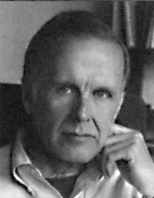
\includegraphics[height=1.9cm]{languages/pix/backus.jpg}% 
  \quad %\vspace*{1ex}
  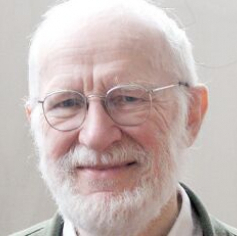
\includegraphics[height=1.9cm]{languages/pix/naur.jpg}}% 
  \wrapcaption{\label{fig:backus}\href{https://en.wikipedia.org/wiki/John_Backus}{John Backus 1924--2007}\index{Backus, J!picture} 与 \label{fig:naur}\href{https://en.wikipedia.org/wiki/Peter_Naur}{Peter Naur 1928--2016}\index{Naur, P!picture}}
\end{wrapfigure}


对文法（即短语结构和造句规则）的研究有着悠久的历史，最早可以追溯到公元前五世纪。
包括 A. Thue 和 E. Post 在内的数学家，在二十世纪初开始将其系统化为重写规则。
这里介绍的这个变体是在 20 世纪 50 年代末，由 J. Backus（约翰·巴科斯）创制，P. Naur（彼得·诺尔）亦有贡献，作为早期计算机语言 ALGOL60 设计工作的一部分。
自那时起，这些规则已成为
\citetext{描述文法的最常用方式}{%
  影响其被采用的一个因素，是 D. Knuth 写给《ACM 通讯》的一封信 \autocite{KnuthCACM}。
  他列举了 BNF 相对于当时广泛使用的文法描述方法的一些优点。
  最重要的是，他对比了 BNF 使用诸如 `\texttt{<addition operator>}` 这样的描述性文本来表示句法范畴，而不是像 `\texttt{A}` 这样的符号，
  并指出这一差异极大地增强了“语法的\textit{解释力}”。
  他还提议了“Backus Naur Form”这个名字。
  （现在最常见的是带有连字符的形式。）
}.\footnote{%
  BNF 的定义较为宽泛。
  虽然有标准，但资料往往并不完全符合任何单一标准。}

% \margingraphic[r]{0.15\textwidth}{languages/pix/naur.jpg}{\label{fig:naur}\href{https://en.wikipedia.org/wiki/Peter_Naur}{Peter Naur 1928--2016}}\index{Naur, P!picture}
与\zcref{sec:Grammars}的一个区别在于排版。
包括 `$\rightarrow$' 在内的元字符，在当时的标准键盘上无法输入。
% The advantage of having metacharacters not on a keyboard is that
% most likely all of the language characters are typeable
% so there is no need to distinguish, say, between the pipe character $\str{|}$
% when used as a part of a language and when used as a metacharacter.
% But the disadvantage lies in having to type the untypeable.
% In the end the convenience of having typeable characters 
% won over the technical gain of having to typographically distinguish 
% metacharacters.\index{metacharacter}
% For instance, for a long time standard keyboards had no arrows
BNF 取而代之使用了 `\bnfsymbol'。\footnote{%
  另一个排版问题是，虽然许多作者和我们一样使用尖括号加斜体来书写非终结符，但也有些作者仅仅依赖不同的字体样式或颜色，或者干脆用大写字母来表示非终结符。}
% (These adjustments were made by P~Naur as editor of the ALGOL60 
% report.)

\begin{example}
下面这个用于具有有限小数部分的实数的 Backus–Naur 范式（BNF）文法扩展了\zcref{ex:grammarForNaturals}。
\begin{grammar}
\ntrm{finite-real} \bnfproduces{}  \trm{-}\ntrm{fraction}
        \syntaxor \trm{+}\ntrm{fraction} 
        \syntaxor \ntrm{fraction}                

\ntrm{fraction} 
     \bnfproduces{} \ntrm{natural} 
       \syntaxor \ntrm{natural}\trm{.}\ntrm{natural}     

\ntrm{natural} 
     \bnfproduces{} \ntrm{digit} 
       \syntaxor \ntrm{digit}\ntrm{natural}     

\ntrm{digit} 
     \bnfproduces{} \trm{0} \syntaxor $\ldots$ \trm{9}     
\end{grammar}
\str{2.718} 的如下推导是最右推导。
\begin{displayedsteps}
  \initialstep\ntrm{finite-real}
  \derives\ntrm{fraction}
  \derives\ntrm{natural}\trm{.}\ntrm{natural}            
  \derives\ntrm{natural}\trm{.}\ntrm{digit}\ntrm{natural}
  \derives\ntrm{natural}\trm{.}\ntrm{digit}\ntrm{digit}\ntrm{natural}  
  \derives\ntrm{natural}\trm{.}\ntrm{digit}\ntrm{digit}\ntrm{digit}
  \derives\ntrm{natural}\trm{.}\ntrm{digit}\ntrm{digit}\trm{8}  
  \derives\ntrm{natural}\trm{.}\ntrm{digit}\trm{18}
  \derives\ntrm{natural}\trm{.718} 
  \derives\trm{2.718}
\end{displayedsteps}
下面是 \trm{0.577} 的一个推导，它既不是最左推导，也不是最右推导。
\begin{displayedsteps}
  \initialstep\ntrm{finite-real}
  \derives\ntrm{fraction}
  \derives\ntrm{natural}\trm{.}\ntrm{natural}            
  \derives\ntrm{natural}\trm{.}\ntrm{digit}\ntrm{natural}
  \derives\ntrm{natural}\trm{.5}\ntrm{natural}  
  \derives\ntrm{natural}\trm{.5}\ntrm{digit}\ntrm{natural}
  \derives\ntrm{digit}\trm{.5}\ntrm{digit}\ntrm{natural} 
  \derives\ntrm{digit}\trm{.5}\ntrm{digit}\ntrm{digit}  
  \derives\ntrm{digit}\trm{.5}\ntrm{digit}\trm{7}
  \derives\trm{0.5}\ntrm{digit}\trm{7} 
  \derives\trm{0.577}
\end{displayedsteps}
\end{example}

\begin{example}
\citetext{时间是一个棘手的工程问题}{% 
  %see https://zachholman.com/talk/utc-is-enough-for-everyone-right
  时间的复杂性有很多方面，其中之一便是闰秒。
  地球因潮汐的制动作用而不断减速。
  地球的平均减速幅度大约为每个世纪每天减慢 $1.4$ 毫秒，尽管具体数值因年而异，取决于包括大地震和火山喷发在内的许多因素。
  为确保原子钟时间与地球自转时间相差不超过 $0.9$ 秒，民用时间偶尔会增加额外的一秒。
  这个闰秒可以是正的也可以是负的，具体取决于地球的自转\Dash 有时会出现仅有 $58$ 秒的分钟，有时则会出现 $60$ 秒的分钟。

  更添混乱的是，自转变化并不均匀，我们无法预测遥远的未来的闰秒。
  国际地球自转服务会发布公告，提前几周通知将要增加的闰秒。
  因此，没有办法确定当前时刻到（例如）十年后之间一共会有多少秒。
  （这会引发诸如导航和高频交易等领域的麻烦，因此有提议要取消闰秒或用闰小时替代。）
  自1972年首次引入闰秒以来，所有的闰秒都是正的，在截至2006年1月的34年间共增加了23个闰秒。
  \autocite{web:USNO}}。
其中一个问题是时间的表示，该领域的一个标准是 \citetext{RFC~3339}{\autocite{rfc3339}}，即《互联网上的日期与时间：时间戳》。
它使用 \citetext{诸如 \str{1958-10-12T23:20:50.52Z} 这样的串}{%
  这种格式有许多优点，包括人类可读性好、对这些串进行排序时较早的时间排在前面、格式简单（只有一种格式），以及包含时区信息。}。
以下是 \citetext{其 BNF 文法}{%
  几点说明：
  (1)~协调世界时是民用时间的基础，常被称为 UTC，但有时也缩写为 Z，读作“Zulu”；
  (2)~年份用四位数字以防止 Y2K 问题 \autocite{y2k}；
  (3)~允许的月份数字仅为 $01$--$12$，且每个月中只允许特定的日期数字；
  (4)~允许的小时仅为 $00$--$23$，分钟必须在 $00$--$59$ 的范围内，等等。 \autocite{rfc3339}} 的部分内容。
%(See \zcref{exer:GrammarsForSmallLangs} for some nonterminals.)
（它包含了下文将讨论的元字符扩展。）

% % https://www.ietf.org/rfc/rfc3339.txt
   % date-month      = 2DIGIT  ; 01-12
   % date-mday       = 2DIGIT  ; 01-28, 01-29, 01-30, 01-31 based on
   %                           ; month/year
   % time-hour       = 2DIGIT  ; 00-23
   % time-minute     = 2DIGIT  ; 00-59
   % time-second     = 2DIGIT  ; 00-58, 00-59, 00-60 based on leap second
   %                           ; rules
   % time-secfrac    = "." 1*DIGIT
   % time-numoffset  = ("+" / "-") time-hour ":" time-minute
   % time-offset     = "Z" / time-numoffset

   % partial-time    = time-hour ":" time-minute ":" time-second
   %                   [time-secfrac]
   % full-date       = date-fullyear "-" date-month "-" date-mday
   % full-time       = partial-time time-offset

   % date-time       = full-date "T" full-time
\begin{grammar}
\ntrm{date-fullyear} \bnfproduces{} \ntrm{4-digits}

\ntrm{date-month} \bnfproduces{} \ntrm{2-digits}

\ntrm{date-mday} \bnfproduces{} \ntrm{2-digits} 

\ntrm{time-hour} \bnfproduces{} \ntrm{2-digits}

\ntrm{time-minute} \bnfproduces{} \ntrm{2-digits}  

\ntrm{time-second} \bnfproduces{} \ntrm{2-digits} 

\ntrm{time-secfrac} \bnfproduces{} \trm{.} \ntrm{1-or-more-digits}

\ntrm{time-numoffset} \bnfproduces{} (\trm{+}\syntaxor\trm{-}) \ntrm{time-hour} \trm{:} \ntrm{time-minute}

\ntrm{time-offset} \bnfproduces{} \trm{Z} \syntaxor \ntrm{time-numoffset}

\ntrm{partial-time} \bnfproduces{} \ntrm{time-hour} \trm{:} \ntrm{time-minute} \trm{:} \ntrm{time-second} [\ntrm{time-secfrac}]

\ntrm{full-date} \bnfproduces{} \ntrm{date-fullyear} \trm{-} \ntrm{date-month} \trm{-} \ntrm{date-mday}

\ntrm{full-time} \bnfproduces{} \ntrm{partial-time} \ntrm{time-offset}

\ntrm{date-time} \bnfproduces{} \ntrm{full-date} \trm{T} \ntrm{full-time}
\end{grammar}
\end{example}

有许多扩展的 Backus–Naur 范式记法，它们已不仅仅是简单的字符替换。
上面的 `\ntrm{partial-time}` 规则展示了其中一种，它使用方括号作为元字符，表示 `\ntrm{time-secfrac}` 是可选的。
这是一种非常常见的结构：另一个例子是下面带有可选 `\str{else}` 的 `\str{if $\ldots$ then $\ldots$}` 语法描述。

\begin{grammar}
    \ntrm{if-stmt} \bnfproduces{}  \trm{if} \ntrm{boolean-expr} \trm{then}
                             \ntrm{stmt-sequence}\\*
                        \quad[ \trm{else}
                             \ntrm{stmt-sequence} ]
                        \ntrm{end-if} \trm{;}
\end{grammar}

为了表示“零次或多次”的重复，BNF 使用 Kleene 星，~$\kleenestar{}$\!。

\begin{grammar}
 \ntrm{string} \bnfproduces{} \ntrm{letter}\trm{*}
\end{grammar}

为了表达“一次或多次”，BNF 使用加号~\trm{+}。

\begin{example} \label{ex:PythonFloatingPoint}
这个关于 Python 浮点数的文法同时展示了方括号和加号。

\begin{grammar}
\ntrm{floatnumber}   \bnfproduces{}  \ntrm{pointfloat} \syntaxor \ntrm{exponentfloat}

\ntrm{pointfloat}    \bnfproduces{}  [\ntrm{intpart}] \ntrm{fraction} \syntaxor \ntrm{intpart} \trm{.}

\ntrm{exponentfloat} \bnfproduces{}  (\ntrm{intpart} \syntaxor \ntrm{pointfloat}) \ntrm{exponent}

\ntrm{intpart}       \bnfproduces{}  \ntrm{digit}+

\ntrm{fraction}      \bnfproduces{}  \trm{.} \ntrm{digit}+

\ntrm{exponent}      \bnfproduces{}  (\trm{e}\syntaxor{}\trm{E}) [\trm{+}\syntaxor{}\trm{-}] \ntrm{digit}+
\end{grammar}

\noindent 在 \ntrm{pointfloat} 规则中，第一个 \ntrm{intpart} 是可选的。
而一个 \ntrm{intpart} 由一个或多个数字组成。
\end{example}

这些扩展并非必需，因为即使没有它们，我们也能表达这些文法。
例如，我们可以将下面这个使用 Kleene 星的文法

\begin{grammar}
 \ntrm{string} \bnfproduces{} \ntrm{letter}\trm{*}
\end{grammar}

\noindent 替换为如下文法。

\begin{grammar}
\ntrm{string} \bnfproduces{} \ntrm{letter}\ntrm{string} \syntaxor \emptystring 
\end{grammar}

\noindent 但这些构造出现的频率足够高，采用缩写形式会带来极大的便利。

从文法到其语法分析器的转换是机械性的过程。
有些程序将文法（通常是 BNF 形式的）作为输入，并输出能够对符合该文法格式的文件进行语法分析的源代码。
这种程序称为 \definend{语法分析器生成器（parser-generator）}\index{parser-generator} 
（有时也被称为
\definend{编译器的编译器（compiler-compiler）},\index{compiler-compiler}
这个词很有趣，但有误导性，因为语法分析器只是编译器的一部分）。

\medskip
总而言之，
BNF 能够表达我们通常想要表达的语言范围（上下文无关文法），
并且能够平滑地转化为语法分析器。
它的优点是简洁，同时在需要保持清晰的地方又不牺牲清晰性。
也就是说，BNF 是一种“阻抗匹配”\Dash 它契合我们的需求。

\begin{exercises}
\recommended


\begin{exercise}
美国的 ZIP 编码有五位数字，末尾可能还有一个短横线和额外的四位数字。
给出一个 BNF 文法。
\begin{answer}\verified
\begin{grammar}
\ntrm{zip} \bnfproduces{} \ntrm{digit}\ntrm{digit}\ntrm{digit}\ntrm{digit}\ntrm{digit}[-\ntrm{digit}\ntrm{digit}\ntrm{digit}\ntrm{digit}]

\ntrm{digit} \bnfproduces{} \trm{0} \syntaxor $\ldots${} \syntaxor \trm{9}    
\end{grammar}
\end{answer}
\end{exercise}

\begin{exercise}
使用 $\Sigma=\set{\str{a},\ldots\,\str{z}}$ 写一个回文语言的 BNF 文法。
\begin{answer}\verified
当我们在前面添加一个字符时，也同时在后面添加它。
\begin{grammar}
\ntrm{palindrome} \bnfproduces{} \trm{a} \ntrm{palindrome} \trm{a} 
    \syntaxor \trm{b} \ntrm{palindrome} \trm{b} 
    \syntaxor $\ldots${}
       \trm{z} \ntrm{palindrome} \trm{z} 
   \syntaxor \ntrm{letter} \syntaxor \emptystring

\ntrm{letter} \bnfproduces{} \trm{a} \syntaxor $\ldots${} 
  \trm{z}    
\end{grammar}
注意，这里将 \emptystring{} 也视作回文。
\end{answer}
\end{exercise}

\recommended


\begin{exercise}
在某大学，课程代码的格式类似于 `MA~208' 或 `PSY~101'，其中院系代码是两到三个大写字母，课程号是三位数字。
给出一个 BNF 文法。
\begin{answer}\verified
这是一种写法。
\begin{grammar}
\ntrm{course code} \bnfproduces{} \ntrm{dept} \ntrm{space} \ntrm{course-number}

\ntrm{dept} \bnfproduces{} \ntrm{two-letter} \syntaxor \ntrm{three-letter} 

\ntrm{two-letter} \bnfproduces{} \ntrm{letter}\ntrm{letter}

\ntrm{three-letter} \bnfproduces{} \ntrm{two-letter}\ntrm{letter}

\ntrm{course-number} \bnfproduces{} \ntrm{digit}\ntrm{digit}\ntrm{digit}

\ntrm{digit} \bnfproduces{} \trm{0} \syntaxor $\ldots${} \trm{9}       

\ntrm{letter} \bnfproduces{} \trm{A} \syntaxor $\ldots${} \trm{Z}       
\end{grammar}
非终结符 \ntrm{space} 生成一个难以直观显示的空格。

我们也可以像下面这样，逐个列举院系名称。
\begin{grammar}
\ntrm{dept} \bnfproduces{} \trm{MA} \syntaxor \trm{PSY} \syntaxor $\ldots${}
\end{grammar}
这种做法更符合实际，不会允许无意义的院系名称。
但其维护上的劣势在于，如果院系代码发生变化，文法描述也必须随之修改。
（在文法中强制要求符合实际往往要付出代价。）
\end{answer}
\end{exercise}

\recommended

\begin{exercise}
\zcref{ex:PythonFloatingPoint}使用了一些 BNF 便利缩写。
\begin{exparts*}
\item
给出与 \ntrm{pointfloat} 等价，但不使用方括号的规则。
\item
类似地，替换 \ntrm{intpart} 规则中的重复算子，以及 \ntrm{exponent} 规则中的方括号和重复算子。
\end{exparts*}
\begin{answer}\verified
\begin{exparts}
\item
可以这样改写。

\begin{grammar}
\ntrm{pointfloat} \bnfproduces{} \ntrm{intpart} \ntrm{fraction} 
    \syntaxor \ntrm{fraction} 
    \syntaxor \ntrm{intpart} \trm{.}
\end{grammar}
\item
用递归来替换 $+$ 算子。
\begin{grammar}
\ntrm{intpart} \bnfproduces{} \ntrm{intpart} \ntrm{digit} 
    \syntaxor \ntrm{digit} 
\end{grammar}
对于 \ntrm{exponent}，列举各种情况。
\begin{grammar}
\ntrm{exponent} \bnfproduces{}
    \trm{e} \ntrm{intpart}  
    \syntaxor \trm{e+} \ntrm{intpart} 
    \syntaxor \trm{e-} \ntrm{intpart} 
    \syntaxor \trm{E} \ntrm{intpart} 
    \syntaxor \trm{E+} \ntrm{intpart} 
    \syntaxor \trm{E-} \ntrm{intpart} 
\end{grammar} 
\end{exparts}
\end{answer}
\end{exercise}

\recommended


\begin{exercise}
在罗马数字中，
字母 I, V, X, L, C, D 和 M 分别代表数值
$1$、$5$、$10$、$50$、$100$、$500$ 和 $1000$。
我们用这些字母从左到右按数值降序排列来表示自然数，
因此 XVI 代表的数在十进制记法中是 $16$，
而 M{}D{}C{}C{}C{}C{}L{}V{}I{}I{}I 代表 $1958$。
我们总是写尽可能短的字符串，
因此我们不会写 I{}I{}I{}I{}I，因为可以改写为 V。
然而，由于我们没有值大于 $1000$ 的符号，
所以必须用很多 M 来表示大数。
\begin{exparts}
\item
给出一个能生成合理的罗马数字串的文法。
\item
罗马数字也常以减法记法书写：例如，$4$ 表示为 I{}V，
因为在表盘等场合，四个 I 与三个 I 很难区分。
在这种记法中，$9$ 是 I{}X，
$40$ 是 X{}L，
$90$ 是 X{}C，
$400$ 是 C{}D，
$900$ 是 C{}M。
给出一个扩展的 BNF 文法，用于生成这种记法中可能出现的字符串。
\end{exparts}
\begin{answer}\verified
\begin{exparts}
\item
这是标准表示法的文法。
\begin{grammar}
\ntrm{roman-numeral} \bnfproduces{} \ntrm{thousands} \ntrm{hundreds} \ntrm{tens} \ntrm{ones}

\ntrm{thousands} \bnfproduces{} \trm{M}\trm{*}     

\ntrm{hundreds} \bnfproduces{} \trm{C} \syntaxor \trm{CC} \syntaxor \trm{CCC} 
   \syntaxor \trm{CCCC}  \syntaxor \trm{D}  \syntaxor \trm{DC}  
   \syntaxor \trm{DCC}  \syntaxor \trm{DCCC}  \syntaxor \trm{DCCCC} 
   \syntaxor \emptystring{}

\ntrm{tens} \bnfproduces{} \trm{X} \syntaxor \trm{XX} \syntaxor \trm{XXX}
    \syntaxor \trm{XXXX}  \syntaxor \trm{L} \syntaxor \trm{LX}
    \syntaxor \trm{LXX}  \syntaxor \trm{LXXX}  \syntaxor \trm{LXXXX}
    \syntaxor \emptystring{}

\ntrm{ones} \bnfproduces{} \trm{I} \syntaxor \trm{II} \syntaxor \trm{III}
     \syntaxor \trm{IIII}  \syntaxor \trm{V}  \syntaxor \trm{VI}  \syntaxor \trm{VII}
      \syntaxor \trm{VIII}  \syntaxor \trm{VIIII}  \syntaxor \emptystring{} 
\end{grammar}
\item
这是减法记法的罗马数字文法。

\begin{grammar}
\ntrm{roman-numeral} \bnfproduces{} \ntrm{thousands} \ntrm{hundreds} \ntrm{tens} \ntrm{ones}

\ntrm{thousands} \bnfproduces{} \trm{M}\trm{*}     

\ntrm{hundreds} \bnfproduces{} \trm{CM} \syntaxor \trm{CD} \syntaxor (\trm{D} \syntaxor \emptystring) (\emptystring \syntaxor \trm{C} \syntaxor \trm{CC} \syntaxor \trm{CCC} )   

\ntrm{tens} \bnfproduces{} \trm{XC} \syntaxor \trm{XL} \syntaxor ( \trm{L}| \emptystring ) ( \emptystring\syntaxor \trm{X} \syntaxor \trm{XX} \syntaxor \trm{XXX})  

\ntrm{ones} \bnfproduces{} \trm{IX} \syntaxor \trm{IV} \syntaxor ( \trm{V} 
  \syntaxor \emptystring ) ( \emptystring \syntaxor \trm{I} \syntaxor \trm{II} \syntaxor \trm{III} )            
\end{grammar}
\end{exparts}
\end{answer}
\end{exercise}

\begin{exercise}
\begin{credit}
  \url{http://people.cs.ksu.edu/~schmidt/300s05/Lectures/GrammarNotes/bnf.html}
\end{credit}
下面的文法描述了一种类 C 的小型编程语言。
\begin{grammar}
\ntrm{program} \bnfproduces{} \trm{\{} \ntrm{statement-list} \trm{\}}

\ntrm{statement-list} \bnfproduces{} [ \ntrm{statement} \trm{;} ]\trm{*}

\ntrm{statement} \bnfproduces{} \ntrm{data-type} \ntrm{identifier}
               \othersyntax \ntrm{identifier} \trm{=} \ntrm{expression}
	       \othersyntax \trm{print} \ntrm{identifier}
	       \othersyntax \trm{while} \ntrm{expression} \trm{\{} \ntrm{statement-list} \trm{\}}

\ntrm{data-type} \bnfproduces{} \trm{int} \syntaxor \trm{boolean}

\ntrm{expression} \bnfproduces{} \ntrm{identifier} \syntaxor \ntrm{number} \syntaxor \trm{(} \ntrm{expression} \ntrm{operator} \ntrm{expression} \trm{)}

\ntrm{identifier} \bnfproduces{}  \ntrm{letter} [ \ntrm{letter} ]\trm{*}

\ntrm{number} \bnfproduces{}  \ntrm{digit} [ \ntrm{digit} ]\trm{*}

\ntrm{operator} \bnfproduces{} \trm{+} \syntaxor \trm{==}

\ntrm{letter} \bnfproduces{} \trm{A} \syntaxor $\ldots${} \syntaxor \trm{Z}

\ntrm{digit} \bnfproduces{} \trm{0} \syntaxor $\ldots${} \syntaxor \trm{9}    
\end{grammar}
\begin{exparts}
\item 为下面的程序给出一个推导和语法分析树。
\begin{lstlisting}
{ int A ;
  A = 1 ;  
  print A ;
}
\end{lstlisting}
% \item Give a parse tree for this program.
% \begin{lstlisting}
% { int A ;
%   A = 5 ;
%   while  ( A == 5 )  { int B ; B = 6 ;  A = ( B + A ) ;
%                        print A ; } ;
%   boolean C ;  print C ;
% }
% \end{lstlisting}
\item 所有程序都必须被花括号包围吗？  
\end{exparts}
\begin{answer}\verified
  \begin{exparts}
  \item 下面是一个推导。为了简洁起见，我们做了缩写，例如在第三行一次性放入了多个
    \ntrm{statement}，而不是逐个放入。
  \begin{displayedsteps}
    \initialstep\ntrm{program}
    \derives\trm{\{} \ntrm{statement-list} \trm{\}}
    \\
    \derives\trm{\{} \ntrm{statement} \trm{;} \ntrm{statement} \trm{;} \ntrm{statement} \trm{;} \trm{\}}
    \\
    \derives\trm{\{} \ntrm{data-type} \ntrm{identifier} \trm{;} \ntrm{statement} \trm{;} \ntrm{statement} \trm{;} \trm{\}}
    \\
    \derives\trm{\{} \trm{int} \ntrm{identifier} \trm{;} \ntrm{statement} \trm{;} \ntrm{statement} \trm{;} \trm{\}}
    \\
    \derives\trm{\{} \trm{int} \ntrm{letter} \trm{;} \ntrm{statement} \trm{;} \ntrm{statement} \trm{;} \trm{\}}
    \\
    \derives\trm{\{} \trm{int} \trm{A} \trm{;} \ntrm{statement} \trm{;} \ntrm{statement} \trm{;} \trm{\}}
    \\
    \derives\trm{\{} \trm{int} \trm{A} \trm{;} \ntrm{identifier} \trm{=} \ntrm{expression} \trm{;} \ntrm{statement} \trm{;} \trm{\}}
    \\
    \derives\trm{\{} \trm{int} \trm{A} \trm{;} \ntrm{letter} \trm{=} \ntrm{expression} \trm{;} \ntrm{statement} \trm{;} \trm{\}}
    \\
    \derives\trm{\{} \trm{int} \trm{A} \trm{;} \trm{A} \trm{=} \ntrm{expression} \trm{;} \ntrm{statement} \trm{;} \trm{\}}
    \\
    \derives\trm{\{} \trm{int} \trm{A} \trm{;} \trm{A} \trm{=} \ntrm{number} \trm{;} \ntrm{statement} \trm{;} \trm{\}}
    \\
    \derives\trm{\{} \trm{int} \trm{A} \trm{;} \trm{A} \trm{=} \ntrm{digit} \trm{;} \ntrm{statement} \trm{;} \trm{\}}
    \\
    \derives\trm{\{} \trm{int} \trm{A} \trm{;} \trm{A} \trm{=} \trm{1} \trm{;} \ntrm{statement} \trm{;} \trm{\}}
    \\
    \derives\trm{\{} \trm{int} \trm{A} \trm{;} \trm{A} \trm{=} \trm{1} \trm{;} \trm{print} \ntrm{identifier} \trm{;} \trm{\}}
    \\
    \derives\trm{\{} \trm{int} \trm{A} \trm{;} \trm{A} \trm{=} \trm{1} \trm{;} \trm{print} \ntrm{letter} \trm{;} \trm{\}}
    \\
    \derives\trm{\{} \trm{int} \trm{A} \trm{;} \trm{A} \trm{=} \trm{1} \trm{;} \trm{print} \trm{A} \trm{;} \trm{\}}
  \end{displayedsteps}
  语法分析树见\figureref{fig:CLikeLang}。
  \begin{figure}
    \centering
    \includegraphics{languages/asy/parsetree/parsetree1000.pdf}
    \caption{类 C 语言的语法分析树}
    \label{fig:CLikeLang}
  \end{figure}
  \item 是的，因为所有推导都必须从 \ntrm{program} 出发并经过
    \ntrm{statement-list}，这迫使它们带有花括号。
  \end{exparts}
\end{answer}
\end{exercise}

\begin{exercise}
下面是一个 LISP 的文法。
\begin{grammar}
\ntrm{s-expression} \bnfproduces{} \ntrm{atomic-symbol}
                   \othersyntax\trm{(} \ntrm{s-expression} \trm{.} \ntrm{s-expression} \trm{)}
                   \othersyntax \ntrm{list}

\ntrm{list} \bnfproduces{} \trm{(} \ntrm{s-expression}\trm{*} \trm{)}

\ntrm{atomic-symbol} \bnfproduces{} \ntrm{letter} \ntrm{atom-part}

\ntrm{atom-part} \bnfproduces{} \ntrm{empty}
                \othersyntax \ntrm{letter} \ntrm{atom-part}
                \othersyntax \ntrm{number} \ntrm{atom-part}

\ntrm{letter} \bnfproduces{} \trm{a} \syntaxor \trm{b} \syntaxor $\ldots${}  \trm{z}

\ntrm{number} \bnfproduces{} \trm{1} \syntaxor \trm{2} \syntaxor $\ldots${}  \trm{9}   
\end{grammar}
此外还有一条规则：\ntrm{empty} 产生一个空格 
\mbox{\trm{" "}}。
推导 s-表达式 \str{(cons (car x) y)}。
\begin{answer}\verified
  在下面的部分推导中，我们做了一些缩写，例如一次性放入多个 \ntrm{s-expression} 来形成
  \ntrm{list}，而不是每次只放一个。
  \begin{displayedsteps}
    \initialstep\ntrm{s-expression}
    \derives \ntrm{list}
    \\
    \derives\trm{(} \ntrm{s-expression} \ntrm{s-expression} \ntrm{s-expression} \trm{)}
    \\
    \derives\trm{(} \ntrm{s-expression} \ntrm{list} \ntrm{s-expression} \trm{)}
    \\
    \derives\trm{(} \ntrm{s-expression} \trm{(} \ntrm{s-expression} \ntrm{s-expression} \trm{)} \ntrm{s-expression} \trm{)}
    \\
    \derives\trm{(} \ntrm{atomic-symbol} \trm{(} \ntrm{s-expression} \ntrm{s-expression} \trm{)} \ntrm{s-expression} \trm{)}
    \\
    \derives\trm{(} \ntrm{letter} \ntrm{atom-part} \trm{(} \ntrm{s-expression} \ntrm{s-expression} \trm{)} \ntrm{s-expression} \trm{)}
    \\
    \derives\trm{(} \ntrm{letter} \ntrm{letter} \ntrm{atom-part} \trm{(} \ntrm{s-expression} \ntrm{s-expression} \trm{)} \ntrm{s-expression} \trm{)}
    \\
    \derives\trm{(} \ntrm{letter} \ntrm{letter} \ntrm{letter} \ntrm{atom-part} \trm{(} \ntrm{s-expression} \ntrm{s-expression} \trm{)} \ntrm{s-expression} \trm{)}
    \\
    \derives\trm{(} \ntrm{letter} \ntrm{letter} \ntrm{letter} \ntrm{letter} \ntrm{atom-part} \trm{(} \ntrm{s-expression} \ntrm{s-expression} \trm{)} \ntrm{s-expression} \trm{)}
    \\
    \derives\trm{(} \ntrm{letter} \ntrm{letter} \ntrm{letter} \ntrm{letter}  \ntrm{atom-part}  \trm{(} \ntrm{s-expression} \ntrm{s-expression} \trm{)} \ntrm{s-expression} \trm{)}
    \\
    \derives\trm{(} \trm{c} \ntrm{letter} \ntrm{letter} \ntrm{letter}  \ntrm{atom-part} \trm{(} \ntrm{s-expression} \ntrm{s-expression} \trm{)} \ntrm{s-expression} \trm{)}
    \\
    \derives\trm{(} \trm{c} \trm{o} \ntrm{letter} \ntrm{letter}  \ntrm{atom-part}  \trm{(} \ntrm{s-expression} \ntrm{s-expression} \trm{)} \ntrm{s-expression} \trm{)}
    \\
    \derives\trm{(} \trm{c} \trm{o} \trm{n} \ntrm{letter}  \ntrm{atom-part}  \trm{(} \ntrm{s-expression} \ntrm{s-expression} \trm{)} \ntrm{s-expression} \trm{)}
    \\
    \derives\trm{(} \trm{c} \trm{o} \trm{n} \trm{s}  \ntrm{atom-part} \trm{(} \ntrm{s-expression} \ntrm{s-expression} \trm{)} \ntrm{s-expression} \trm{)}
    \\
    \derives\trm{(} \trm{c} \trm{o} \trm{n} \trm{s}  \ntrm{empty} \trm{(} \ntrm{s-expression} \ntrm{s-expression} \trm{)} \ntrm{s-expression} \trm{)}
    \\
    \derives\trm{(} \trm{c} \trm{o} \trm{n} \trm{s}  \trm{" "} \trm{(} \ntrm{s-expression} \ntrm{s-expression} \trm{)} \ntrm{s-expression} \trm{)}
  \end{displayedsteps}
  将剩余的非终结符展开为字母很繁琐，因此我们到此为止。
\end{answer}
\end{exercise}

\begin{exercise}
Python 3的格式规范迷你语言（Format Specification Mini-Language）用于描述字符串替换。
\begin{grammar}
  \ntrm{format-spec} \bnfproduces{}  [[\ntrm{fill}]\ntrm{align}][\ntrm{sign}][\trm{\#}][\trm{0}][\ntrm{width}][\ntrm{gr}][\trm{.}\ntrm{precision}][\ntrm{type}]

\ntrm{fill}            \bnfproduces{}  \ntrm{any character}

\ntrm{align}           \bnfproduces{}  \trm{<} \syntaxor \trm{>} \syntaxor \trm{=} \syntaxor \trm{\^{}}

\ntrm{sign}            \bnfproduces{}  \trm{+} \syntaxor \trm{-} \syntaxor \trm{ }

\ntrm{width}           \bnfproduces{}  \ntrm{integer}

\ntrm{gr} \bnfproduces{}  \trm{-} \syntaxor \trm{,}

\ntrm{precision}       \bnfproduces{}  \ntrm{integer}

\ntrm{type}            \bnfproduces{}  \trm{b} \syntaxor \trm{c} \syntaxor \trm{d} \syntaxor \trm{e} \syntaxor \trm{E} \syntaxor \trm{f} \syntaxor \trm{F} \syntaxor \trm{g} \syntaxor \trm{G} \syntaxor \trm{n} \syntaxor \trm{o} \syntaxor \trm{s} \syntaxor \trm{x} \syntaxor \trm{X} \syntaxor \trm{\%}  
\end{grammar}
规定 \ntrm{integer} 可生成
\mbox{\ntrm{digit} \ntrm{integer}}
或 \ntrm{digit}。
为以下字符串给出推导过程：
\begin{exparts*}
\item \str{03f}
\item \str{+\#02X}.
\end{exparts*}
\begin{answer}\verified
\begin{exparts}
\item
  例如，这里我们将利用 BNF 记法一次替换多个非终结符，而不是每次只替换一个。
  \begin{displayedsteps}
    \initialstep\ntrm{format-spec}
    \derives \trm{0} \ntrm{width} \ntrm{type}
    \\
    \derives \trm{0} \ntrm{integer} \ntrm{type}
    \\
    \derives \trm{0} \ntrm{digit} \ntrm{type}
    \\
    \derives \trm{0} \trm{3} \ntrm{type}
    \\
    \derives \trm{0} \trm{3} \trm{f}
  \end{displayedsteps}
\item
  \begin{displayedsteps}
    \initialstep\ntrm{format-spec}
    \derives \ntrm{sign} \trm{\#} \trm{0} \ntrm{width} \ntrm{type}
    \\
    \derives \trm{+} \trm{\#} \trm{0} \ntrm{width} \ntrm{type}
    \\
    \derives \trm{+} \trm{\#} \trm{0} \ntrm{integer} \ntrm{type}
    \\
    \derives \trm{+} \trm{\#} \trm{0} \ntrm{digit} \ntrm{type}
    \\
    \derives \trm{+} \trm{\#} \trm{0} \trm{2} \ntrm{type}
    \\
    \derives \trm{+} \trm{\#} \trm{0} \trm{2} \trm{X}
  \end{displayedsteps}
\end{exparts}
\end{answer}
\end{exercise}

% \begin{exercise}
% This is the grammar of BNF, written in BNF.
% \begin{grammar}
% \ntrm{syntax}         \bnfproduces{} \ntrm{rule} \syntaxor \ntrm{rule} \ntrm{syntax}

%  \ntrm{rule}           \bnfproduces{} \ntrm{opt-whitespace} \trm{<} \ntrm{rule-name} \trm{>} \ntrm{opt-whitespace} \trm{::=} \ntrm{opt-whitespace} \ntrm{expression} \ntrm{line-end}

%  \ntrm{opt-whitespace} \bnfproduces{} \trm{" "} \ntrm{opt-whitespace} \syntaxor \emptystring{}

%  \ntrm{expression}     \bnfproduces{} \ntrm{list} \syntaxor \ntrm{list} \ntrm{opt-whitespace} \trm{|} \ntrm{opt-whitespace} \ntrm{expression}

%  \ntrm{line-end}       \bnfproduces{} \ntrm{opt-whitespace} \ntrm{EOL} \syntaxor \ntrm{line-end} \ntrm{line-end}

%  \ntrm{list}           \bnfproduces{} \ntrm{term} \syntaxor \ntrm{term} \ntrm{opt-ws} \ntrm{list}

%  \ntrm{term}           \bnfproduces{} \ntrm{literal} \syntaxor \trm{<} \ntrm{rule-name} \trm{>}

%  \ntrm{literal}        \bnfproduces{} \textdoublequote{} \ntrm{text1} \textdoublequote{} \syntaxor \textsinglequote{} \ntrm{text2} \textsinglequote{}

%  \ntrm{text1}          \bnfproduces{} \emptystring \syntaxor \ntrm{character1} \ntrm{text1}

%  \ntrm{text2}          \bnfproduces{} \emptystring \syntaxor \ntrm{character2} \ntrm{text2}

%  \ntrm{character}      \bnfproduces{} \ntrm{letter} \syntaxor \ntrm{digit} \syntaxor \ntrm{symbol}

%  \ntrm{letter}         \bnfproduces{} \trm{A} \syntaxor \trm{B} \syntaxor \ldots{} \trm{z} 

% % \trm{C} \syntaxor \trm{D} \syntaxor \trm{E} \syntaxor \trm{F} \syntaxor \trm{G} \syntaxor \trm{H} \syntaxor \trm{I} \syntaxor \trm{J} \syntaxor \trm{K} \syntaxor \trm{L} \syntaxor \trm{M} \syntaxor \trm{N} \syntaxor \trm{O} \syntaxor \trm{P} \syntaxor \trm{Q} \syntaxor \trm{R} \syntaxor \trm{S} \syntaxor \trm{T} \syntaxor \trm{U} \syntaxor \trm{V} \syntaxor \trm{W} \syntaxor \trm{X} \syntaxor \trm{Y} \syntaxor \trm{Z} \syntaxor \trm{a} \syntaxor \trm{b} \syntaxor \trm{c} \syntaxor \trm{d} \syntaxor \trm{e} \syntaxor \trm{f} \syntaxor \trm{g} \syntaxor \trm{h} \syntaxor \trm{i} \syntaxor \trm{j} \syntaxor \trm{k} \syntaxor \trm{l} \syntaxor \trm{m} \syntaxor \trm{n} \syntaxor \trm{o} \syntaxor \trm{p} \syntaxor \trm{q} \syntaxor \trm{r} \syntaxor \trm{s} \syntaxor \trm{t} \syntaxor \trm{u} \syntaxor \trm{v} \syntaxor \trm{w} \syntaxor \trm{x} \syntaxor \trm{y} \syntaxor \trm{z}

%  \ntrm{digit}          \bnfproduces{} \trm{0} \syntaxor \trm{1} \syntaxor 
%                        \ldots{} \trm{9}

% % \trm{2} \syntaxor \trm{3} \syntaxor \trm{4} \syntaxor \trm{5} \syntaxor \trm{6} \syntaxor \trm{7} \syntaxor \trm{8} \syntaxor \trm{9}

%  \ntrm{symbol}         \bnfproduces{}  \trm{|} \syntaxor \emptystring \syntaxor \trm{-} \syntaxor \trm{!} \syntaxor \trm{\#} \syntaxor \trm{\$} \syntaxor \trm{\%} \syntaxor \trm{\&} \syntaxor \trm{(} \syntaxor \trm{)} \syntaxor \trm{*} \syntaxor \trm{+} \syntaxor \trm{,} \syntaxor \trm{-} \syntaxor \trm{.} \syntaxor \trm{/} \syntaxor \trm{:} \syntaxor \trm{;} \syntaxor \trm{<} \syntaxor \trm{=} \syntaxor \trm{>} \syntaxor \trm{?} \syntaxor \trm{@} \syntaxor \trm{[} \syntaxor \trm{\textbackslash} \syntaxor \trm{]} \syntaxor \trm{\textasciicircum} \syntaxor \trm{-} \syntaxor \trm{`} \syntaxor \trm{{} \syntaxor \trm{\syntaxor} \syntaxor \trm{}} \syntaxor \trm{\textasciitilde}

%  \ntrm{character1}     \bnfproduces{} \ntrm{character} \syntaxor \trm{'}

%  \ntrm{character2}     \bnfproduces{} \ntrm{character} \syntaxor \textdoublequote

%  \ntrm{rule-name}      \bnfproduces{} \ntrm{letter} \syntaxor \ntrm{rule-name} \ntrm{rule-char}

%  \ntrm{rule-char}      \bnfproduces{} \ntrm{letter} \syntaxor \ntrm{digit} \syntaxor \trm{-}
% \end{grammar}
% \begin{exparts}
% \item Give a derivation of the rule \mbox{\ntrm{ab} \bnfproduces{} \ntrm{cd} e}.  
% \item Give a derivation of the rule \mbox{\ntrm{ab} \bnfproduces{} e \ntrm{cd}}.  
% \end{exparts}
% \end{exercise}
\end{exercises}
\index{BNF|)}

\extra{图遍历}\index{Graph traversal|(}\index{tree!traversal}\index{directed acyclic graph DAG!traversal} \label{extra:GraphTraversal}
在本书的多处，我们将描述如何遍历树或其他图。
例如，当我们描述枚举集合 $\N\times\N$ 的 Cantor 对应时，我们画了下面这个阵列。
\begin{equation*}
  \begin{array}{cccccc}
    \vdots          &\vdots         &\vdots         &\vdots         \\
    \sequence{0,3}  &\sequence{1,3} &\sequence{2,3} &\sequence{3,3} &\cdots  \\
    \sequence{0,2}  &\sequence{1,2} &\sequence{2,2} &\sequence{3,2} &\cdots  \\ 
    \sequence{0,1}  &\sequence{1,1} &\sequence{2,1} &\sequence{3,1} &\cdots  \\ 
    \sequence{0,0}  &\sequence{1,0} &\sequence{2,0} &\sequence{3,0} &\cdots
  \end{array}
\end{equation*}
我们可以将每个阵列元素与其上方的元素、以及与其右方的元素连接起来，从而构成一个图。
这里我们将左下角旋转到了顶部。


\begin{center}
  \vcenteredhbox{\includegraphics{languages/asy/graphs/graphs1031.pdf}}
\end{center}


这并不是一棵树，因为有些顶点之间存在不止一条路，例如
$\sequence{0,0}\to\sequence{0,1}\to\sequence{1,1}$
和
$\sequence{0,0}\to\sequence{1,0}\to\sequence{1,1}$。
相反，它是一个有向无环图。
% But it is like a tree in that there are no cycles.

Cantor 的枚举


\begin{center}
  \begin{tabular}{r|ccccccc@{\hspace{6pt}}c}
    \tabulartext{编号}
       &$0$    &$1$   &$2$  &$3$  &$4$  &$5$  &$6$ &\ldots
   \\ \cline{2-9}
    \tabulartext{数对}
               &$\sequence{0,0}$\rule{0pt}{10pt}
               &$\sequence{0,1}$
               &$\sequence{1,0}$
               &$\sequence{0,2}$
               &$\sequence{1,1}$
               &$\sequence{2,0}$
               &$\sequence{0,3}$
               &\ldots
     \end{tabular}
\end{center}


从上到下遍历此图。

我们将介绍两种遍历策略：
\definend{深度优先}\index{depth-first traversal}\index{graph!traversal!depth-first}
和
\definend{广度优先}。\index{breadth-first traversal}\index{graph!traversal!breadth-first}
下面的树展示了这两种策略。
表中第一行先访问一个节点的子节点，再去访问该节点的兄弟节点。
表中第二行先访问所有深度为 $k$ 的节点，再访问任何深度为 $k+1$ 的节点。（在一棵树中，一个节点的
\definend{深度}\index{graph!node!rank}\index{rank of a vertex}
是指从根节点到该节点的最短路中的边数。
在这个有向无环图中，它是指从源节点到该节点的最短路中的边数。）


\begin{center}
  \vcenteredhbox{\includegraphics{languages/asy/graphs/graphs1028.pdf}}
  \qquad
  \begin{tabular}{r|l}
    \multicolumn{1}{c}{\tabulartext{遍历方式}}
      &\multicolumn{1}{c}{\tabulartext{节点顺序}}  \\
    \hline 
    深度优先\rule{0pt}{11pt}
      &$a$-$b$-$e$-$f$-$c$-$d$-$g$-$i$-$j$-$h$ \\
    广度优先
      &$a$-$b$-$c$-$d$-$e$-$f$-$g$-$h$-$i$-$j$ \\
  \end{tabular}
  % \vcenteredhbox{\includegraphics{languages/asy/graphs/graphs1030.pdf}}
  % \qquad
  % \vcenteredhbox{\includegraphics{languages/asy/graphs/graphs1029.pdf}}
\end{center}

这里我们将编写 Racket 代码来遍历树和有向无环图。
代码首先定义一个 \codeinline{node}，本质上是一个有序对。
\lstinputlisting[firstline=15,lastline=15]{\traversefile}
Racket 的 \codeinline{struct} 构造会自动定义许多有用的函数。
其中一个是创建函数 \codeinline{(node n s)}，它用于创建节点。
它还创建了访问器函数 \codeinline{node-name} 和 \codeinline{node-children}，我们将在下面看到。

我们使用该创建函数来定义下一个函数。
\lstinputlisting[firstline=21,lastline=22]{\traversefile}
注意 \codeinline{children} 被创建为一个集合，以便我们可以快速访问其成员。
将这个集合设为可变的，意味着在创建树的过程中，我们可以向该集合中添加子节点来修改它。

我们使用那个例程来创建新树和单源有向无环图。
\lstinputlisting[firstline=27,lastline=28]{\traversefile}

下一个例程接收一个节点作为输入，并将一个子节点添加到它的子节点集合中。
（LISP 家族语言通常会在过程名末尾加上感叹号，这些过程的主要作用不是返回某个值，而是产生副作用，例如修改数据结构。）
\lstinputlisting[firstline=34,lastline=37]{\traversefile}

有了这些，我们可以构建上面所示的十节点树。\footnote{%
  我们建立的是从父节点到子节点的边，而没有反向的边。
  因此该图是有向的。
  }
\lstinputlisting[firstline=96,lastline=110]{\traversefile}
以下代码返回了前面展示的 Cantor 数组的有限部分。
\lstinputlisting[firstline=127,lastline=144]{\traversefile}

为了演示遍历代码，在每个节点我们将只打印节点名称，
\lstinputlisting[firstline=46,lastline=47]{\traversefile}
缩进 $2\cdot r$ 个空格，其中 $r$ 是深度。
\lstinputlisting[firstline=41,lastline=42]{\traversefile}

我们从深度优先开始。它是递归的，运行 \codeinline{fcn} 然后在每个子节点上调用自身。
\lstinputlisting[firstline=86,lastline=94]{\traversefile}
Racket 和其他 LISP 派生语言允许我们传递函数。当我们运行这个例程时，我们将传递 \codeinline{show-node-name} 作为 \codeinline{fcn}。

% Note the optional keyword argument \codeinline{maximumrank},
% with \codeinline{MAXIMUM-RANK} as its default.
% This a convenience for testing and development, 
% to keep the routine from running away.
% \lstinputlisting[firstline=50,lastline=50]{\traversefile}

这是深度优先例程的运行结果。
\begin{lstlisting}
> (define t (sample-tree-make))
> (traverse-dfs t 0 show-node-name)
a
  b
    e
    f
  c
  d
    h
    g
      i
      j
\end{lstlisting}
集合是无序的，所以当我们显示元素时，输出的顺序可能与输入的顺序不同。

现在介绍广度优先遍历。它由两个函数组成：\codeinline{traverse-bfs} 和 \codeinline{traverse-bfs-helper}\!。
在 Scheme 派生语言（如 Racket）中，例程通常组织为一个调用者和一个辅助函数。
这是因为辅助函数是 \definend{尾递归的}。\index{tail recursion}
它的最后一步操作是递归调用，而在 Scheme 语言中，编译器知道可以将这样的例程转换为迭代的可执行代码。
这结合了递归的表达能力和迭代内存消耗恒定的优点。

\codeinline{traverse-bfs-helper} 的策略是一次遍历一层，其中一层是所有相同深度的节点的集合。
当例程遍历 \codeinline{level} 的成员时，为下一次调用，它将所有这些节点的子节点存储在列表 \codeinline{next-level} 中。
\lstinputlisting[firstline=70,lastline=84]{\traversefile}
这一策略不会使例程沿圈游走（例如回到根节点），因为树和有向无环图都没有圈。

这是在示例树上运行例程的结果。
\begin{lstlisting}
> (define t (sample-tree-make))
> (traverse-bfs t show-node-name)
a
  b
  c
  d
    h
    e
    f
    g
      i
      j
\end{lstlisting}
最后，这是 Cantor 有向无环图的遍历。
\begin{lstlisting}
> (define t (cantor-DAG-make))
> (traverse-bfs t show-node-name)
0,0
  0,1
  1,0
    2,0
    1,1
    0,2
      3,0
      2,1
      1,2
      0,3
\end{lstlisting}

\begin{exercises}


\begin{exercise}
这是一个 \definend{二叉树}，因为每个节点要么有两个子节点，要么没有
（在某些定义中，作者也允许只有一个子节点）。
\begin{center}
  \vcenteredhbox{\includegraphics{languages/asy/graphs/graphs1032.pdf}}
\end{center}
\begin{exparts}
\item 给出定义这棵树的 Racket 代码。
\item 执行深度优先遍历。
\item 执行广度优先遍历。
\end{exparts}
\begin{answer}\verified
\begin{exparts}
\item 以下是代码。
\lstinputlisting[firstline=119,lastline=130]{\traversefile}
\item 运行定义后，从解释器得到以下输出。
\begin{lstlisting}
> (define t (binary-tree-make))
> (traverse-dfs t 0 show-node-name)
a
  c
    g
      i
      h
    f
  b
    e
    d
\end{lstlisting}
\item 我们得到这个。
\begin{lstlisting}
> (define t (binary-tree-make))
> (traverse-bfs t show-node-name)
a
  c
  b
    e
    d
    g
    f
      i
      h
\end{lstlisting}
\end{exparts}
\end{answer}
\end{exercise}

\end{exercises}
\index{Graph traversal|)}

\endinput
% ===============================================================

\extra{Lambda 演算与 Scheme}
% See http://matt.might.net/articles/compiling-up-to-lambda-calculus/

% Jim Larson
% 1996-07-26
% This talk was given at the JPL Section 312 Programming Lunchtime Seminar.

函数接受输入并产生输出。
假设我们有一个“巧克力包裹”函数，根据对应的输入产生如下输出：
% \begin{grammar}
%   \str{peanuts} &\produces  \str{chocolate-covered peanuts} \\
%   \str{rasins}  &\produces  \str{chocolate-covered rasins} \\
%   \str{ants}    &\produces \str{chocolate-covered ants}
% \end{grammar}
我们可以用 $\lambda$-演算来描述这样的函数。
\begin{equation*}
	\lambda x.\str{chocolate-covered $x$}
\end{equation*}
这是一个\definend{$\lambda$-表达式}。

要将函数应用于自变量，使用以下语法。
% \begin{equation*}
%   (\lambda x.\str{chocolate-covered $x$})\,\str{peanuts} 
%     \produces \str{chocolate-covered peanuts}
% \end{equation*}
函数也可以是 $\lambda$-表达式应用于自变量所得到的结果，就像下面这个“包裹函数制造器”一样。
\begin{equation*}
  \lambda y.\lambda x.\str{$y$-covered $x$}
\end{equation*}
用它来创建一个焦糖包裹函数。
% \begin{align*}
%   (\lambda y.\lambda x.\str{$y$-covered $x$})\,\str{caramel} 
%     &\produces \lambda x.\str{caramel-covered $x$}   \\
%   (\lambda x.\str{caramel-covered $x$})\,\str{peanuts} 
%     &\produces \str{caramel-covered peanuts}
% \end{align*}
函数也可以是其他函数的输入，就像下面这个“施加于蚂蚁”函数一样。
\begin{equation*}
	\lambda f.(f)\,\str{ants}
\end{equation*}
我们可以将巧克力包裹函数传递给“施加于蚂蚁”函数：
% \begin{multline*}
% 	(\lambda f.\str{$(f)$ants})\lambda x.\str{chocolate-covered $x$}  \\
%       \begin{split}
%         \hspace*{3em}
% 	&\produces (\lambda x.\str{chocolate-covered $x$})\str{ants}  \\
% 	&\produces \str{chocolate-covered ants}
%       \end{split}
% \end{multline*}

$\lambda$-表达式具有以下语法。
\begin{lstlisting}
	lambda-expression \bnfproduces{}	variable
				| constant
				| application
				| abstraction
	application \bnfproduces{} (lambda-expression)lambda-expression
	abstraction \bnfproduces{} Lvariable.lambda-expression
\end{lstlisting}
$\lambda$-表达式的求值基于两条归约规则的应用。
\definend{$\alpha$-归约}规则指出，我们可以一致地重命名被绑定的变量：
% \begin{equation*}
% 	\lambda x.E \produces \text{$\lambda z.\{z/x\}E$ 
%                         for any $z$ which is neither free nor bound in $E$}
% \end{equation*}
其中 $\{z/x\}E$ 表示将 $E$ 中 $x$ 的所有自由出现替换为 $z$。
\definend{$\beta$-归约}规则指出，将 $\lambda$-表达式应用于自变量，就是用该自变量一致地替换其体部中的约束变量：
\begin{equation*}
	(\lambda x.P)Q -> [Q/x]P
\end{equation*}
其中 $[Q/x]P$ 表示将 $P$ 中 $x$ 的所有自由出现替换为 $Q$。

Church-Rosser 定理指出，一系列替换的最终结果不依赖于这些替换执行的顺序。

\subsection{$\lambda$-演算的通用性}
$\lambda$-演算是计算的一个通用模型，也就是说，任何能在 Turing 机上表达的计算，也都能在 $\lambda$-演算中表达。

为了说明这一点，下面展示了如何将条件控制结构翻译为 $\lambda$-演算。
\begin{align*}
	\str{true} &= \lambda x.\lambda y.x  \\
	\str{false} &= \lambda x.\lambda y.y        \\
	\str{if-then-else} &= \lambda a.\lambda b.\lambda c.((a)b)c 
\end{align*}
下面是这些规则的一个应用示例。
% \begin{multline*}
% 	(((\str{if-then-else})\str{false})\str{apple})\str{banana}  \\
%       \begin{split}
%         \qquad 
% 	&\produces (((\lambda a.\lambda b.\lambda c.((a)b)c)\lambda x.\lambda y.y)\str{apple})\str{banana}       \\
% 	&\produces ((\lambda b.\lambda c.((\lambda x.\lambda y.y)b)c)\str{apple})\str{banana}          \\
% 	&\produces (\lambda c.((\lambda x.\lambda y.y)\str{apple})c)\str{banana}  \\
% 	&\produces ((\lambda x.\lambda y.y)\str{apple})\str{banana}   \\
% 	&\produces (\lambda y.y)\str{banana}    \\
% 	&\produces \str{banana}
%      \end{split}
% \end{multline*}
下面是一些数据结构操作的翻译示例。
\begin{align*}
	\str{cons} &= \lambda a.\lambda b.\lambda c.((c)a)b   \\
	\str{head} &= \lambda x.(x)\str{true}                  \\
	\str{tail} &= \lambda x.(x)\str{false}               \\
          \\
	0 &= \lambda f.\lambda x.x    \\
	1 &= \lambda f.\lambda x.(f)x  \\
	2 &= \lambda f.\lambda x.(f)(f)x   \\
	3 &= \lambda f.\lambda x.(f)(f)(f)x    \\
        \\
	\str{succ} &= \lambda n.\lambda f.\lambda x.(f)((n)f)x  \\
	+ &= \lambda m.\lambda n.\lambda f.\lambda x.((m)f)((n)f)x   \\
	* &= \lambda m.\lambda n.\lambda f.(m)(n)f           \\
	\str{zero?} &= \lambda n.((n)(\str{true})\str{false})\str{true} \\
	\str{pred} &= \lambda n.(((n)\lambda p.\lambda z.((z)(\str{succ})(p)\str{true})(p)\str{true})Lz.((z)0)0)\str{false}
\end{align*}

最后，你可以用\definend{$Y$ 组合子}创建递归函数。
\begin{gather*}
	Y = \lambda y.(\lambda x.(y)(x)x)\lambda x.(y)(x)x        \\
	(Y)E -> (E)(Y)E -> \cdots -> (E)\ldots (E)(Y)E
\end{gather*}
我们需要它来创建递归函数，例如阶乘函数：
\begin{equation*}
	\str{fact} = \lambda n.(((\str{if-then-else})(\str{zero?})n)1)((*)n)(\str{fact})(\str{pred})n
\end{equation*}
照这样写是行不通的，因为 \str{fact} 在其自身定义中是一个自由变量！我们需要某种方式将 \str{fact} 绑定到“这个函数本身”，这可以用 $Y$ 组合子来实现。
\begin{equation*}
	\str{fact} = (Y)\lambda f.\lambda n.(((\str{if-then-else})(\str{zero?})n)1)((*)n)(f)(\str{pred})n
        \end{equation*}

\subsection{从理论到编程语言}
尽管 $\lambda$-演算强大到足以表达任何程序，但这并不意味着人们真的想这么做。
毕竟，Turing 机也提供了同样强大的计算基础。

$\lambda$-演算的优势在于，它能在一个更丰富的原语世界之上，轻松地用作“胶水”。
它作为胶水的优势在于：它与人们的编程方式有着自然的对应关系，且自然的编译技术能生成高性能代码。
后者是通过尾调用和续传递等优化实现的，这些是此处未涵盖的更高级主题。

以 $\lambda$-演算“粘合”的语言具有软件工程上的优势。
$\lambda$-表达式可以局部地理解——它们对环境的依赖完全通过其自由变量体现。
与可比的命令式代码相比，$\lambda$-表达式往往具有更少的自由变量和更多的约束变量，因为它们并不那么依赖赋值来表达计算。
命令式程序通过修改某个全局可访问的值存储来推进。
相比之下，函数式程序则通过函数应用和值的返回来推进。
这消除了与维护全局值存储相关的许多类错误。

\subsection{Scheme}
Scheme 编程语言本质上是上面概述的 $\lambda$-演算，外加以下特性：

\begin{itemize}
\item
    $\lambda$-表达式一次绑定多个参数的能力。
\item
    一组丰富的常量，因此数字、算术、数据结构等不必凭空构建。
\item
    基本的控制结构，因此控制操作不必凭空构建。
\item
    如有需要，还提供一个赋值操作。
\item
    一个已定义名称的环境，以支持交互使用、重定义，以及无需使用 $Y$ 组合子的递归定义。
\item
    一个带有 I/O 操作的库，用以连接程序和外部世界。
\end{itemize}

在 Scheme 中，程序看起来就像数据结构——两者都是由列表构建的。一个列表看起来像：
\begin{equation*}
	(\str{elt1}\ \str{elt2}\ \ldots{}\ \str{eltn})
\end{equation*}
其中每个元素要么是一个原子（数字或符号），要么是另一个列表。

$\lambda$-演算中的表达式翻译如下：
% \begin{align*}
% 	\lambda x.M  &\becomes  \text{\codeinline!(lambda (x) M)!} \\
% 	(M)N  &\becomes  \text{\codeinline!(M N)!}
% \end{align*}
此外，Scheme 允许多参数的 $\lambda$-表达式和函数应用。
\begin{lstlisting}
(lambda (a b c) (+ a (* b c)))
\end{lstlisting}
\codeinline!define! 语法在局部环境中将名称绑定到值：
\begin{lstlisting}
(define pi 3.14159265)
(define fact
    (lambda (n)
        (if (zero? n)
        1
        (* n (fact (- n 1))))))
(define alpha (sin (/ pi 180)))
\end{lstlisting}
一些 Scheme 结构是语法糖，也就是说，这些表达式可以被转化为由更基本的运算符构成的表达式。
\codeinline!let! 构造允许初始化和绑定局部变量，使得下式 \begin{lstlisting}
(let ((x1 E1)
      (x2 E2)
      (x3 E3))
      \ldots{}body\ldots{} )
\end{lstlisting} 等价于下式 \begin{lstlisting}
((lambda (x1 x2 x3) \ldots{}body\ldots{} )
E1
E2
E3)
\end{lstlisting}。
% Definition of a function can be done without an explicit lambda-expression
% \begin{lstlisting}
% 	(define (f x y z)	=>	(define f
% 	  \ldots{}body\ldots{})			  (lambda (x y z)
% 					    \ldots{}body\ldots{}))
% \end{lstlisting}

\subsection{Scheme 中的标准习惯用法}
在像 C 或 Pascal 这样的传统块结构的命令式语言中，会这样写：
\begin{lstlisting}
begin
    x := 1;
    y := 2 * some_global_var;
    z := some_function();
    \ldots{}body using x, y, and z\ldots{}
end
\end{lstlisting}
而 Scheme 则会使用 \codeinline!let! 语法来绑定局部变量。
\begin{lstlisting}
(let ((x 1)
    (y (* 2 some-global-var))
    (z (some-function)))
    ..body using x, y, and z\ldots{})
\end{lstlisting}
正如我们在上面看到的，\codeinline!let! 构造仅仅是对 \codeinline!lambda! 和函数应用的一种风格化使用，目的是为体部创建一个环境，在这个环境中局部变量被绑定到它们的值。
注意，这种编程风格要求局部变量在使用之前初始化。

Scheme 不强调诸如 \codeinline!do! 这样的迭代结构，而偏爱递归函数调用。
一种称为尾递归的特殊优化能产生与循环等价的编译代码。
\begin{lstlisting}
(define (new-fact n)
    (define (iter n a)
    (if (zero? n)
        a
        (iter (- n 1) (* n a))))
    (iter n 1))
\end{lstlisting}
与等价的 C 函数作比较：
\begin{lstlisting}
int
new_fact(int n)
{
    int a = 1;
    while (n != 0)
        a *= n--;
    return a;
}
\end{lstlisting}
注意，C 版本中的循环不能独立理解\Dash 要弄清楚 \codeinline!n! 和 \codeinline!a! 是什么，我们必须查看整个函数；而在 Scheme 版本中，\codeinline!iter! 函数可以从 \codeinline!new-fact! 函数中提取出来并独立理解\Dash 它没有自由变量！
对于像这样的玩具示例，这可能显得不太重要，但随着函数规模和循环复杂度的增加，这种模块性就显得重要了。

尽管每次需要一个循环时都要定义一个新函数，可能看起来是不必要且笨拙的，但一些常见的用法本身就可以转化为函数。
例如，Scheme 中一个常见的操作是：取出一个列表，对其中每个元素应用一个函数，从而形成一个由结果组成的新列表。
\begin{lstlisting}
(define (list-of-squares l)
    (define (iter l)
        (if (null? l)
            (quote ())
            (cons ((lambda (x) (* x x)) (car l)) (iter (cdr l)))))
    (iter l))
\end{lstlisting}
这种迭代属于习惯用法，因此我们可以将其封装到一个函数中：
\begin{lstlisting}
(define (map f l)
    (define (iter l)
        (if (null? l)
            (quote ())
            (cons (f (car l)) (iter (cdr l)))))
        (iter l))

(define (list-of-squares l)
    (map (lambda (x) (* x x)) l))
\end{lstlisting}
我们也可以在 C 中编写这个程序，使用将函数指针作为参数传递给其他函数的技术。
然而，C 语言的某些特性使得这很困难。
假设我们需要一个对一列数字进行仿射变换 $Ax + B$ 的函数，其中 A 和 B 是该函数的参数。
在 C 中我们必须这样写：
\begin{lstlisting}
double A, B;	/* global variables */
static double
affine(double x)
{
    return A * x + B;
}

List *
affinelist(double a, double b, List *l)
{
    A = a;
    B = b;
    return map(&affine, l);
}
\end{lstlisting}
由于在 C 中，\codeinline!map! 函数只接受一个函数指针，变换参数必须保存在某个静态位置，以便仿射函数能找到它们。
这导致代码不可重入\Dash 同一时刻只能有一个 \codeinline!affinelist! 调用处于活动状态。

Pascal 允许在块内声明函数，并且可以访问该块内可见的所有变量。
在一种“块结构”变体的 C 语言中，我们可以这样做：
\begin{lstlisting}
List *
affinelist(double a, double b, List *l)
{
    double
    affine(double x)
    {
        return a * x + b;
    }
    return map(&affine, l);
}
\end{lstlisting}
这使得该函数可重入。
但 Scheme 在使用这些局部函数方面赋予了我们更大的自由\Dash 它们甚至在父函数返回后依然可以存在！
由父函数绑定的变量仍然可以被这些局部函数访问（且只能被它们访问），这实际上创建了一个不透明对象，而局部函数就是访问其状态的方法。
这为我们提供了一种在 Scheme 中使用高阶函数进行面向对象编程的方法。

假设我们想要创建一个具有状态变量 \codeinline!svN! 和方法 \codeinline!methodN! 的对象。
\begin{lstlisting}
(define (make-object sv1 sv2 ... svN)
    (lambda (mesg)
        (cond ((eq? mesg (quote method1)) (lambda args1 body1))
               ((eq? mesg (quote method2)) (lambda args2 body2))
                 ...
               ((eq? mesg (quote methodM)) (lambda argsM bodyM))
               (else (error "Unknown method for object")))))

(define (method1 obj args1) ((obj (quote method1)) args1))
    ...
\end{lstlisting}
所以，对象是一个过程，它接受一条消息，并动态地返回一个将处理该消息的过程。
每个过程都可以访问用于创建该对象的状态变量。
多个实例是通过多次调用 \codeinline!make-object! 函数创建的。
类结构和继承可以通过委托来实现。
因此，使用高阶函数可以以一种自然的方式实现面向对象代码。

以下是一些基于 $\lambda$-演算的编程语言的优点。

\begin{itemize}
\item
    清晰的数学基础。语言的形式化规约无需依赖具体的机器或编译器。
\item
    许多常见的编程惯用法有自然的表示形式。
\item
    通过高阶函数实现高级编程。
\item
    与高级数学对象（如泛函）直接对应。
\item
    高效的机器实现。
\item
    程序的模块化程度更高\Dash 它们可以在局部被理解和分析。 
\end{itemize}

当然也存在一些不足。

\begin{itemize}
\item
    现实中的实现往往未能达到应有的水平。
\item
    语言所提供的计算模型与底层机器的现实情况相距甚远。这有利有弊。
\item
    在其他语言中简单的事情，在 Scheme 中往往很难做到；而一些简单的 Scheme 技巧在其他语言中也很难实现。
\item
    使用完整的 $\lambda$-演算进行编程，需要在运行时系统中包含垃圾回收器。这会导致：
        比 Fortran 或 C 更复杂的运行时系统；
        难以与用其他语言编译的代码进行链接；
        给实时或交互式使用带来的复杂性。 
\end{itemize}
